\mysection{\HelloWorldSectionName}
\label{sec:helloworld}

Utilizziamo il famoso esempio dal libro [\KRBook]:

\lstinputlisting[style=customc]{patterns/01_helloworld/hw.c}

\subsection{x86}

\EN{\subsubsection{MSVC}

Let's compile it in MSVC 2010:

\begin{lstlisting}
cl 1.cpp /Fa1.asm
\end{lstlisting}

(The \TT{/Fa} option instructs the compiler to generate an assembly listing file)

\begin{lstlisting}[caption=MSVC 2010,style=customasmx86]
CONST	SEGMENT
$SG3830	DB	'hello, world', 0AH, 00H
CONST	ENDS
PUBLIC	_main
EXTRN	_printf:PROC
; Function compile flags: /Odtp
_TEXT	SEGMENT
_main	PROC
	push	ebp
	mov	ebp, esp
	push	OFFSET $SG3830
	call	_printf
	add	esp, 4
	xor	eax, eax
	pop	ebp
	ret	0
_main	ENDP
_TEXT	ENDS
\end{lstlisting}

MSVC produces assembly listings in Intel-syntax.
The differences between Intel-syntax and AT\&T-syntax will be discussed in \myref{ATT_syntax}.

The compiler generated the file, \TT{1.obj}, which is to be linked into \TT{1.exe}.
In our case, the file contains two segments: \TT{CONST} (for data constants) and \TT{\_TEXT} (for code).

\myindex{\CLanguageElements!const}
\label{string_is_const_char}
The string \TT{hello, world} in \CCpp has type \TT{const char[]}\InSqBrackets{\TCPPPL p176, 7.3.2}, but it does not have its own name.
The compiler needs to deal with the string somehow, so it defines the internal name \TT{\$SG3830} for it.

That is why the example may be rewritten as follows:

\lstinputlisting[style=customc]{patterns/01_helloworld/hw_2.c}

Let's go back to the assembly listing. As we can see, the string is terminated by a zero byte, which is standard for \CCpp strings.
More about \CCpp strings: \myref{C_strings}.

In the code segment, \TT{\_TEXT}, there is only one function so far: \main{}.
The function \main starts with prologue code and ends with epilogue code (like almost any function)
\footnote{You can read more about it in the section about function prologues and epilogues ~(\myref{sec:prologepilog}).}.

\myindex{x86!\Instructions!CALL}
After the function prologue we see the call to the \printf{} function:\\
\INS{CALL \_printf}.
\myindex{x86!\Instructions!PUSH}
Before the call, a string address (or a pointer to it) containing our greeting is placed on the stack with the help of the \PUSH instruction.

When the \printf function returns the control to the \main function, the string address (or a pointer to it) is still on the stack.
Since we do not need it anymore, the \gls{stack pointer} (the \ESP register) needs to be corrected.

\myindex{x86!\Instructions!ADD}
\INS{ADD ESP, 4} means add 4 to the \ESP register value.

Why 4? Since this is a 32-bit program, we need exactly 4 bytes for address passing through the stack. If it was x64 code we would need 8 bytes.
\INS{ADD ESP, 4} is effectively equivalent to \INS{POP register} but without using any register\footnote{CPU flags, however, are modified}.

\myindex{Intel C++}
\myindex{\oracle}
\myindex{x86!\Instructions!POP}

For the same purpose, some compilers (like the Intel C++ Compiler) may emit \TT{POP ECX}
instead of \ADD (e.g., such a pattern can be observed in the \oracle{} code as it is compiled with the Intel C++ compiler).
This instruction has almost the same effect but the \ECX register contents will be overwritten.
The Intel C++ compiler supposedly uses \TT{POP ECX} since this instruction's opcode is shorter than \TT{ADD ESP, x} (1 byte for \TT{POP} against 3 for \TT{ADD}).

Here is an example of using \POP instead of \ADD from \oracle{}:

\begin{lstlisting}[caption=\oracle 10.2 Linux (app.o file),style=customasmx86]
.text:0800029A                 push    ebx
.text:0800029B                 call    qksfroChild
.text:080002A0                 pop     ecx
\end{lstlisting}

%Read more about the stack in section
% ~(\myref{sec:stack}).
\myindex{\CLanguageElements!return}
After calling \printf, the original \CCpp code contains the statement \TT{return 0}~---return 0 as the result of the \main function.

\myindex{x86!\Instructions!XOR}
In the generated code this is implemented by the instruction \INS{XOR EAX, EAX}.

\myindex{x86!\Instructions!MOV}

\XOR is in fact just \q{eXclusive OR}\footnote{\href{http://go.yurichev.com/17118}{Wikipedia}} but the compilers often use it instead of
\INS{MOV EAX, 0}---again because it is a slightly shorter opcode (2 bytes for \XOR against 5 for \MOV).

\myindex{x86!\Instructions!SUB}
Some compilers emit \INS{SUB EAX, EAX}, which means \emph{SUBtract the value in the} \EAX \emph{from the value in} \EAX. That in any case will results in zero.

\myindex{x86!\Instructions!RET}
The last instruction \RET returns the control to the \gls{caller}. Usually, this is \CCpp \ac{CRT} code which in turn returns control to the \ac{OS}.
}
\FR{\subsubsection{MSVC}

Compilons-le avec MSVC 2010:

\begin{lstlisting}
cl 1.cpp /Fa1.asm
\end{lstlisting}

(L'option \TT{/Fa} indique au compilateur de générer un fichier avec le listing en assembleur)

\begin{lstlisting}[caption=MSVC 2010,style=customasmx86]
CONST	SEGMENT
$SG3830	DB	'hello, world', 0AH, 00H
CONST	ENDS
PUBLIC	_main
EXTRN	_printf:PROC
; Function compile flags: /Odtp
_TEXT	SEGMENT
_main	PROC
	push	ebp
	mov	ebp, esp
	push	OFFSET $SG3830
	call	_printf
	add	esp, 4
	xor	eax, eax
	pop	ebp
	ret	0
_main	ENDP
_TEXT	ENDS
\end{lstlisting}

MSVC génère des listings assembleur avec la syntaxe Intel.
La différence entre la syntaxe Intel et la syntaxe AT\&T sera discutée dans \myref{ATT_syntax}.

Le compilateur a généré le fichier object \TT{1.obj}, qui sera lié dans l'exécutable \TT{1.exe}.
Dans notre cas, le fichier contient deux segments: \TT{CONST} (pour les données constantes)
 et \TT{\_TEXT} (pour le code).

\myindex{\CLanguageElements!const}
\label{string_is_const_char}
La chaîne \TT{hello, world} en \CCpp a le type \TT{const char[]}\InSqBrackets{\TCPPPL p176, 7.3.2}, mais
elle n'a pas de nom.
Le compilateur doit pouvoir l'utiliser et lui défini donc le nom interne \TT{\$SG3830} à cette fin.

C'est pourquoi l'exemple pourrait être récrit comme suit:

\lstinputlisting[style=customc]{patterns/01_helloworld/hw_2.c}

Retournons au listing assembleur. Comme nous le voyons, la chaîne est terminée avec un octet à zéro, ce qui
est le standard pour les chaînes \CCpp.

Dans le segment de code, \TT{\_TEXT}, il n'y a qu'une seule fonction: \main{}.
La fonction \main débute par le code du prologue et se termine par le code de l'épilogue 
(comme presque toutes les fonctions)
\footnote{Vous pouvez en lire plus dans la section concernant les prologues et épilogues de
fonctions ~(\myref{sec:prologepilog}).}.

\myindex{x86!\Instructions!CALL}
Après le prologue de la fonction nous voyons l'appel à la fonction \printf{}:\\
\INS{CALL \_printf}.
\myindex{x86!\Instructions!PUSH}
Avant l'appel, l'adresse de la chaîne (ou un pointeur sur elle) contenant notre message
 est placée sur la pile avec l'aide de l'instruction \PUSH.

Lorsque la fonction \printf rend le contrôle à la fonction \main, l'adresse de la chaîne (ou un pointeur sur elle)
est toujours sur la pile.
Comme nous n'en avons plus besoin, le pointeur de pile (\gls{stack pointer} le registre \ESP) doit être corrigé.

\myindex{x86!\Instructions!ADD}
\INS{ADD ESP, 4} signifie ajouter 4 à la valeur du registre \ESP.

Pourquoi 4? puisqu'il s'agit d'un programme 32-bit, nous avons besoin d'exactement 4 octets pour passer une adresse
par la pile. S'il s'agissait d'un code x64, nous aurions besoin de 8 octets.
\INS{ADD ESP, 4} est effectivement équivalent à \INS{POP register} mais sans utiliser de registre\footnote{Les
flags du CPU, toutefois, sont modifiés}.

\myindex{Intel C++}
\myindex{\oracle}
\myindex{x86!\Instructions!POP}

Pour la même raison, certains compilateurs (comme le compilateur C++ d'Intel) peuvent générer \TT{POP ECX}
à la place de \ADD (e.g., ce comportement peut être observé dans le code d'\oracle{} car il est
compilé avec le compilateur C++ d'Intel.
Cette instruction a presque le même effet mais le contenu du registre \ECX sera écrasé.
Le compilateur C++ d'Intel utilise probablement \TT{POP ECX} car l'opcode de cette instruction est plus
 court que celui de \TT{ADD ESP, x} (1 octet pour \TT{POP} contre 3 pour \TT{ADD}).

Voici un exemple d'utilisation de \POP à la place de \ADD dans \oracle{}:

\begin{lstlisting}[caption=\oracle 10.2 Linux (app.o file),style=customasmx86]
.text:0800029A                 push    ebx
.text:0800029B                 call    qksfroChild
.text:080002A0                 pop     ecx
\end{lstlisting}

%Lisez en plus sur la pile dans la section
% ~(\myref{sec:stack}).

\myindex{\CLanguageElements!return}
Après l'appel de \printf, le code \CCpp original contient la déclaration \TT{return 0}~---renvoie 0 comme valeur de retour de la fonction \main.

\myindex{x86!\Instructions!XOR}
Dans le code généré cela est implémenté par l'instruction \INS{XOR EAX, EAX}.

\myindex{x86!\Instructions!MOV}

\XOR est en fait un simple \q{OU exclusif (eXclusive OR}\footnote{\href{http://go.yurichev.com/17118}{Wikipédia}} mais
les compilateurs l'utilisent souvent à la place de \INS{MOV EAX, 0}---à nouveau parce que l'opcode est légèrement plus
court (2 octets pour \XOR contre 5 pour \MOV).

\myindex{x86!\Instructions!SUB}
Certains compilateurs génèrent \INS{SUB EAX, EAX}, qui signifie \emph{Soustraire la valeur dans} \EAX \emph{de la valeur dans} \EAX,
 ce qui, dans tous les cas, donne zéro.

\myindex{x86!\Instructions!RET}
La dernière instruction \RET redonne le contrôle à l'\glslink{caller}{appelant}.
Habituellement, c'est ce code \CCpp \ac{CRT}, qui, à son tour, redonne le contrôle à l'\ac{OS}.

}
\IT{\subsubsection{MSVC}

Compiliamolo in MSVC 2010:

\begin{lstlisting}
cl 1.cpp /Fa1.asm
\end{lstlisting}

(l'opzione \TT{/Fa} indica al compilatore di generare un file con il listato assembly)

\begin{lstlisting}[caption=MSVC 2010,style=customasmx86]
CONST	SEGMENT
$SG3830	DB	'hello, world', 0AH, 00H
CONST	ENDS
PUBLIC	_main
EXTRN	_printf:PROC
; Function compile flags: /Odtp
_TEXT	SEGMENT
_main	PROC
	push	ebp
	mov	ebp, esp
	push	OFFSET $SG3830
	call	_printf
	add	esp, 4
	xor	eax, eax
	pop	ebp
	ret	0
_main	ENDP
_TEXT	ENDS
\end{lstlisting}

MSVC produce codice assembly in sintassi Intel.
La differenza tra le sintassi Intel e AT\&T-syntax sarà discussa al \myref{ATT_syntax}.

Il compilatore ha generato il file, \TT{1.obj}, che deve essere linkato in \TT{1.exe}.
Nel nostro caso, il file contiene due segmenti: \TT{CONST} (per i dati constanti) e \TT{\_TEXT} (per il codice).

\myindex{\CLanguageElements!const}
\label{string_is_const_char}
La stringa \TT{hello, world} in \CCpp ha tipo \TT{const char[]}\InSqBrackets{\TCPPPL p176, 7.3.2}, ma non ha un nome assegnato.
Il compilatore deve in qualche modo aver a che fare con la stringa, e la definisce quindi con il nome interno \TT{\$SG3830}.

Questo è il motivo per cui l'esempio potrebbe essere riscritto nel modo seguente:

\lstinputlisting[style=customc]{patterns/01_helloworld/hw_2.c}

Torniamo al listato assembly. Come possiamo vedere, la stringa è terminata con un byte zero, che è lo standard per la terminazione delle stringhe \CCpp.
Più informazioni sulle stringhe in \CCpp: \myref{C_strings}.

Nel code segment, \TT{\_TEXT}, esiste fino ad ora solo una funzione: \main{}.
La funzione \main inizia con il codice di prologo (prologue code) e termina con il codice di epilogo (epilogue code) (come quasi qualunque funzione)
\footnote{Maggiori informazioni si trovano nella sezione su prologo ed epilogo delle funzioni ~(\myref{sec:prologepilog}).}.

\myindex{x86!\Instructions!CALL}
Dopo il prologo della funzione, notiamo la chiamata alla funzione \printf{} : \INS{CALL \_printf}.
\myindex{x86!\Instructions!PUSH}
Prima della chiamata, l'indirizzo della stringa (o un puntatore ad essa) contenente il saluto viene messo sullo stack con l'aiuto dell'istruzione \PUSH.

Quando la funzione \printf restituisce il controllo alla funzione \main , l'indirizzo della stringa (o il puntatore) si trova ancora sullo stack.
Poichè non ne abbiamo più bisogno, lo \gls{stack pointer} (il registro \ESP ) deve essere corretto.

\myindex{x86!\Instructions!ADD}
\INS{ADD ESP, 4} significa aggiungi 4 al valore del registro \ESP.

Perchè 4? Essendo questo un programma a 32-bit, abbiamo esattamente bisogno di 4 bytes per passare un indirizzo attraverso lo stack. Se fosse stato codice x64 ne sarebbero serviti 8.
\INS{ADD ESP, 4} è a tutti gli effetti equivalente a \TT{POP register} ma senza usare alcun registro\footnote{i flag CPU vengono comunque modificati}.

\myindex{Intel C++}
\myindex{\oracle}
\myindex{x86!\Instructions!POP}

Per lo stesso scopo, alcuni compilatori (come l'Intel C++ Compiler) potrebbero emettere l'istruzione \TT{POP ECX}
invece di \ADD (ad esempio, queto tipo di pattern può essere osservato nel codice di \oracle{} che è compilato con il compilatore Intel C++).
Questa istruzione ha pressoché lo stesso effetto ma il contenuto del registro \ECX sarà sovrascritto.
Il compilatore Intel C++ usa probabilmente \TT{POP ECX} poichè l'opcode di questa istruzione è più corto di \TT{ADD ESP, x} (1 byte per \TT{POP} contro 3 per \TT{ADD}).

Ecco un esempio dell'uso di \POP al posto di \ADD da \oracle{}:

\begin{lstlisting}[caption=\oracle 10.2 Linux (\ITph{}),style=customasmx86]
.text:0800029A                 push    ebx
.text:0800029B                 call    qksfroChild
.text:080002A0                 pop     ecx
\end{lstlisting}

%Read more about the stack in section
% ~(\myref{sec:stack}).
\myindex{\CLanguageElements!return}
Dopo la chiamata a \printf, il codice \CCpp originale contiene la direttiva \TT{return 0}~---restituisci 0 come risultato dalla funzione \main.

\myindex{x86!\Instructions!XOR}
Nel codice generato, questa è implementata dall'istruzione \INS{XOR EAX, EAX}.

\myindex{x86!\Instructions!MOV}

\XOR è infatti semplicemente \q{eXclusive OR, ovvero OR esclusivo}\footnote{\href{http://go.yurichev.com/17118}{wikipedia}} ma i compilatori lo usano spesso al posto di
\INS{MOV EAX, 0}---ancora una volta poichè è un opcode leggermente più corto (2 byte per \XOR contro 5 per \MOV).

\myindex{x86!\Instructions!SUB}
Alcuni compilatori emettono l'istruzione \INS{SUB EAX, EAX}, che significa \emph{sottrai (SUBtract) il valore nel registro} \EAX \emph{dal valore nel registro} \EAX, che, in ogni caso, risulta uguale a zero.

\myindex{x86!\Instructions!RET}
L'ultima istruzione \RET restituisce il controllo al chiamante (\gls{caller}). Solitamente, questo è codice \CCpp \ac{CRT} , che, a sua volta, restituisce il controllo all' \ac{OS}.
}
\NL{\subsubsection{MSVC}

We compileren het in MSVC 2010:

\begin{lstlisting}
cl 1.cpp /Fa1.asm
\end{lstlisting}

(\TT{/Fa} optie zorgt ervoor dat de compiler het bestand met assembly listing genereert)

\begin{lstlisting}[caption=MSVC 2010,style=customasmx86]
CONST	SEGMENT
$SG3830	DB	'hello, world', 0AH, 00H
CONST	ENDS
PUBLIC	_main
EXTRN	_printf:PROC
; Function compile flags: /Odtp
_TEXT	SEGMENT
_main	PROC
	push	ebp
	mov	ebp, esp
	push	OFFSET $SG3830
	call	_printf
	add	esp, 4
	xor	eax, eax
	pop	ebp
	ret	0
_main	ENDP
_TEXT	ENDS
\end{lstlisting}

\NLph{}
Het verschil tussen Intel-syntax en AT\&T-syntax zal besproken worden in: \myref{ATT_syntax}.

De compiler heeft het bestand, \TT{1.obj} gegenereerd, hetwelk gelinkt wordt tot \TT{1.exe}.
In ons geval bevat het bestand twee segmenten: \TT{CONST} (voor data constanten) en \TT{\_TEXT}(voor code).

\myindex{\CLanguageElements!const}
\label{string_is_const_char}
De string \TT{hello, world} in \CCpp is van het type \TT{const char[]}\InSqBrackets{\TCPPPL p176, 7.3.2}, maar heeft geen eigen naam.
De compiler moet een manier hebben om met de string om te kunnen, en definieert er daarom de interne naam \TT{\$SG3830} voor.

Daarom kan het voorbeeld herschreven worden als volgt:

\lstinputlisting[style=customc]{patterns/01_helloworld/hw_2.c}

Laten we terug gaan naar de assembly listing. Zoals je kan zien, wordt de string beeindigd door een nul-byte. Dit is standaard voor \CCpp strings.
Meer over \CCpp strings: \myref{C_strings}.

In het code segment, \TT{\_TEXT}, is er slechts een functie tot nu toe: \main{}.
De functie \main begint met een proloog code en eindigt met een epiloog code (zoals bijna elke functie)
\footnote{Je kan hier meer over lezen in de sectie over functieprologen en epilogen ~(\myref{sec:prologepilog}).}.

\myindex{x86!\Instructions!CALL}
Na de functie proloog zien we de call naar de \printf{} functie: \INS{CALL \_printf}.
\myindex{x86!\Instructions!PUSH}
Voor de call wordt het adres van de string (of een pointer ernaar) die onze begroeting bevat, op de stack geplaatsd met de hulp van de \PUSH instructie.

Wanneer de \printf functie de controle teruggeeft aan de \main functie, staat het string adres (of de pointer ernaar) nog steeds op de stack.
Aangezien we dit niet meer nodig hebben, moet de \gls{stack pointer} (het \ESP register) gecorrigeerd worden.

\myindex{x86!\Instructions!ADD}
\INS{ADD ESP, 4} betekent dat er 4 wordt opgeteld bij de \ESP registerwaarde.

Waarom 4? Aangezien dit een 32-bit programma is, hebben we exact 4 bytes nodig om een adres door te geven via de stack. als het x64 code was, zouden we 8 bytes nodig gehad hebben.
\INS{ADD ESP, 4} is een effectief equivalent voor \TT{POP register} maar zonder gebruik van een register\footnote{CPU flags worden echter wel aangepast}.

\myindex{Intel C++}
\myindex{\oracle}
\myindex{x86!\Instructions!POP}

Met dezelfde reden zullen sommige compilers (zoals de Intel C++ Compiler) gebruik maken van \TT{POP ECX}
in plaats van \ADD (een dergelijk patroon kan waargenomen worden in de \oracle{} code aangezien deze gecompileerd is met de Intel C++ compiler).
Deze instructie heeft bijna hetzelfde effect, maar de inhoud van het \ECX register zal overschreven worden.
De Intel C++ Compiler gebruikt waarschijnlijk \TT{POP ECX} aangezien de opcode van deze instructie korter is dan \TT{ADD ESP, x} (1 byte voor \TT{POP} tegen 3 voor \TT{ADD}).

Hier is een voorbeeld van het gebruik van \POP in plaats van \ADD van \oracle{}:

\begin{lstlisting}[caption=\oracle 10.2 Linux (app.o bestand),style=customasmx86]
.text:0800029A                 push    ebx
.text:0800029B                 call    qksfroChild
.text:080002A0                 pop     ecx
\end{lstlisting}

%Lees meer over de stack in de sectie ~(\myref{sec:stack}).
\myindex{\CLanguageElements!return}
Na \printf aan te roepen, bevat de originele \CCpp code het statement \TT{return 0}~---return 0 als resultaat van de \main functie.

\myindex{x86!\Instructions!XOR}
In de gegenereerde code wordt dit geimplementeerd door de instructie \INS{XOR EAX, EAX}.

\myindex{x86!\Instructions!MOV}

\XOR is feitelijk simpelweg \q{eXclusive OR}\footnote{\href{http://go.yurichev.com/17118}{wikipedia}} maar de compilers gebruiken het vaak in plaats van
\INS{MOV EAX, 0} --- wederom omdat de opcode hiervoor iets korter is (2 bytes voor \XOR tegenover 5 voor \MOV).

\myindex{x86!\Instructions!SUB}
Sommige compilers gebruiken \INS{SUB EAX, EAX}, wat staat voor \emph{verminder de waarde in} \EAX \emph{met de waarde in} \EAX, wat in elke situatie resulteert in nul.

\myindex{x86!\Instructions!RET}
De laatste instructie \RET geeft de controle terug aan de \gls{caller}. Gewoonlijk is dit \CCpp \ac{CRT} code, die op zijn beurt de controle teruggeeft aan het \ac{OS}.

}
\RU{\subsubsection{MSVC}

Компилируем в MSVC 2010:

\begin{lstlisting}
cl 1.cpp /Fa1.asm
\end{lstlisting}

(Ключ \TT{/Fa} означает сгенерировать листинг на ассемблере)

\begin{lstlisting}[caption=MSVC 2010,style=customasmx86]
CONST	SEGMENT
$SG3830	DB	'hello, world', 0AH, 00H
CONST	ENDS
PUBLIC	_main
EXTRN	_printf:PROC
; Function compile flags: /Odtp
_TEXT	SEGMENT
_main	PROC
	push	ebp
	mov	ebp, esp
	push	OFFSET $SG3830
	call	_printf
	add	esp, 4
	xor	eax, eax
	pop	ebp
	ret	0
_main	ENDP
_TEXT	ENDS
\end{lstlisting}

MSVC выдает листинги в синтаксисе Intel.
Разница между синтаксисом Intel и AT\&T будет рассмотрена немного позже:

Компилятор сгенерировал файл \TT{1.obj}, который впоследствии будет слинкован линкером в \TT{1.exe}.
В нашем случае этот файл состоит из двух сегментов: \TT{CONST} (для данных-констант) и \TT{\_TEXT} (для кода).

\myindex{\CLanguageElements!const}
\label{string_is_const_char}
Строка \TT{hello, world} в \CCpp имеет тип \TT{const char[]}\InSqBrackets{\TCPPPL p176, 7.3.2}, однако не имеет имени.
Но компилятору нужно как-то с ней работать, поэтому он дает ей внутреннее имя \TT{\$SG3830}.

Поэтому пример можно было бы переписать вот так:

\lstinputlisting[style=customc]{patterns/01_helloworld/hw_2.c}

Вернемся к листингу на ассемблере. Как видно, строка заканчивается нулевым байтом~--- это требования стандарта \CCpp для строк.
Больше о строках в \CCpp: \myref{C_strings}.

В сегменте кода \TT{\_TEXT} находится пока только одна функция: \main{}.
Функция \main, как и практически все функции, начинается с пролога и заканчивается эпилогом
\footnote{Об этом смотрите подробнее в разделе о прологе и эпилоге функции ~(\myref{sec:prologepilog}).}.

\myindex{x86!\Instructions!CALL}
Далее следует вызов функции \printf{}: \INS{CALL \_printf}.
\myindex{x86!\Instructions!PUSH}
Перед этим вызовом адрес строки (или указатель на неё) с нашим приветствием (``Hello, world!'') при помощи инструкции \PUSH помещается в стек.

После того, как функция \printf возвращает управление в функцию \main, адрес строки (или указатель на неё) всё ещё лежит в стеке.
Так как он больше не нужен, то \glslink{stack pointer}{указатель стека} (регистр \ESP) корректируется.

\myindex{x86!\Instructions!ADD}
\INS{ADD ESP, 4} означает прибавить 4 к значению в регистре \ESP.

Почему 4? Так как это 32-битный код, для передачи адреса нужно 4 байта. В x64-коде это 8 байт.\\
\INS{ADD ESP, 4} эквивалентно \TT{POP регистр}, но без использования какого-либо регистра\footnote{Флаги процессора, впрочем, модифицируются}.

\myindex{Intel C++}
\myindex{\oracle}
\myindex{x86!\Instructions!POP}

Некоторые компиляторы, например, Intel C++ Compiler, в этой же ситуации могут вместо 
\ADD сгенерировать \TT{POP ECX} (подобное можно встретить, например, в коде \oracle{}, им скомпилированном),
что почти то же самое, только портится значение в регистре \ECX.
Возможно, компилятор применяет \TT{POP ECX}, потому что эта инструкция короче (1 байт у \TT{POP} против 3 у \TT{ADD}).

Вот пример использования \POP вместо \ADD из \oracle{}:

\begin{lstlisting}[caption=\oracle 10.2 Linux (файл app.o),style=customasmx86]
.text:0800029A                 push    ebx
.text:0800029B                 call    qksfroChild
.text:080002A0                 pop     ecx
\end{lstlisting}

%О стеке можно прочитать в соответствующем разделе
% ~(\myref{sec:stack}).
\myindex{\CLanguageElements!return}
После вызова \printf в оригинальном коде на \CCpp указано \TT{return 0}~--- вернуть 0 в качестве результата функции \main.

\myindex{x86!\Instructions!XOR}
В сгенерированном коде это обеспечивается инструкцией \\
\INS{XOR EAX, EAX}.

\myindex{x86!\Instructions!MOV}

\XOR, как легко догадаться~--- \q{исключающее ИЛИ}\footnote{\href{http://go.yurichev.com/17118}{wikipedia}}, но компиляторы часто используют его вместо простого
\INS{MOV EAX, 0} --- снова потому, что опкод короче (2 байта у \XOR против 5 у \MOV).

\myindex{x86!\Instructions!SUB}
Некоторые компиляторы генерируют \INS{SUB EAX, EAX}, что значит \emph{отнять значение в} \EAX \emph{от значения в }\EAX, что в любом случае даст 0 в результате.

\myindex{x86!\Instructions!RET}
Самая последняя инструкция \RET возвращает управление в вызывающую функцию. Обычно это код \CCpp \ac{CRT}, который, в свою очередь, вернёт управление в \ac{OS}.

}
\PTBR{\input{patterns/01_helloworld/MSVC_x86_PTBR}}
\DE{\subsubsection{MSVC}

Das Beispiel wird jezt in MSVC 2010 kompiliert:

\begin{lstlisting}
cl 1.cpp /Fa1.asm
\end{lstlisting}

(Die \TT{/Fa}-Option weist den Compiler an, Assembler-Code auszugeben.)

\begin{lstlisting}[caption=MSVC 2010,style=customasmx86]
CONST	SEGMENT
$SG3830	DB	'hello, world', 0AH, 00H
CONST	ENDS
PUBLIC	_main
EXTRN	_printf:PROC
; Function compile flags: /Odtp
_TEXT	SEGMENT
_main	PROC
	push	ebp
	mov	ebp, esp
	push	OFFSET $SG3830
	call	_printf
	add	esp, 4
	xor	eax, eax
	pop	ebp
	ret	0
_main	ENDP
_TEXT	ENDS
\end{lstlisting}

MSVC erstellt Assembler-Code im Intel-Syntax.
Der Unterschied zum AT\&T-Syntax wird später in \myref{ATT_syntax} behandelt.

Der Compiler generiert die Datei \TT{1.obj}, die anschließend zu \TT{1.exe} gelinkt wird.
In diesem Fall besteht die Datei aus zwei Segmenten: \TT{CONST} (für konstante Daten) und \TT{\_TEXT} (für Quellcode).

\myindex{\CLanguageElements!const}
\label{string_is_const_char}
Die Zeichenkette \TT{hello, world} hat in \CCpp den Typ \TT{const char[]}\InSqBrackets{\TCPPPL p176, 7.3.2}, aber keinen eigenen Bezeichner.
Da der Compiler jedoch irgendwie auf diese Zeichenkette zugreifen muss, definiert er den internen Namen \TT{\$SG3830}.

Aus diesem Grund kann das Beispiel auch wie folgt geschrieben werden:

\lstinputlisting[style=customc]{patterns/01_helloworld/hw_2.c}

Nochmal zurück zum Assembler-Listing: wie man sehen kann ist die Zeichenkette gemäß dem \CCpp-Standard mit einem 0-Byte abgeschlossen.
Mehr über \CCpp-Zeichenketten ist im Abschnitt \myref{C_strings} zu finden.

% Not sure what the technically precise translation of prologue and epilogue is
In dem Code-Segment \TT{\_TEXT} ist lediglich eine Funktion: \main{}.
Diese startet mit einem Prolog-Teil und endet mit einem Epilog-Teil (wie fast alle Funktionen)
\footnote{Mehr darüber in dem Abschnitt über Funktions-Prologe und -Epiloge ~(\myref{sec:prologepilog}).}.

\myindex{x86!\Instructions!CALL}
Nach dem Funktions-Prolog ist der Aufruf der \printf{}-Funktion zu sehen:\\
\INS{CALL \_printf}.
\myindex{x86!\Instructions!PUSH}
Vor dem Aufruf wird die Adresse der Zeichenkette (oder ein Zeiger darauf) mit dem Inhalt unserer Begrüßung
auf dem Stack gespeichert. Dies geschieht durch die \PUSH-Anweisung.

Wenn \printf die Ausführung wieder an \main übergibt, befindet sich die Adresse der Zeichenkette (oder ein Zeiger darauf) immer noch auf dem Stack.
Da diese jedoch nicht mehr benötigt wird, muss der \gls{stack pointer} (das \ESP-Register) korrigiert werden.

\myindex{x86!\Instructions!ADD}
\INS{ADD ESP, 4} bedeutet, dass der Wert 4 zu dem \ESP-Rregister-Wert addiert wird.

Warum 4? Da dies ein 32-Bit-Programm ist, werden exakt 4 Byte benötigt um Adressen auf dem Stack abzulegen. Wenn dies x64-Code wäre, würden 8 Byte benötigt.
\INS{ADD ESP, 4} ist quasi gleichbedeutend mit \INS{POP Register} jedoch ohne die Verwendung von Registern\footnote{Statusregister der CPU können sich jedoch ändern}.

\myindex{Intel C++}
\myindex{\oracle}
\myindex{x86!\Instructions!POP}

Aus dem gleichen Grund generieren einige Compiler (wie der Intel C++-Compiler) die Anweisung \TT{POP ECX}
anstatt \ADD (dieses Muster kann zum Beispiel im \oracle{}-Code gefunden werden, da dieser mit dem Intel-Compiler erstellt wurde).
Diese Anweisung hat nahezu den gleichen Effekt, nur dass die Inhalte des \ECX-Registers überschrieben werden.
Der Intel C++-Compiler nutzt \TT{POP ECX} vermutlich, da der OpCode für diese Anweisung kürzer ist als \TT{ADD ESP, x} (1 Byte für \TT{POP} und 3 Byte für \TT{ADD}),

Nachfolgend ein Beispiel unter der Verwendung von \POP anstatt \ADD aus \oracle{}:

\begin{lstlisting}[caption=\oracle 10.2 Linux (app.o file),style=customasmx86]
.text:0800029A                 push    ebx
.text:0800029B                 call    qksfroChild
.text:080002A0                 pop     ecx
\end{lstlisting}

%Mehr über den Stack gibt es im Abschnitt
% ~(\myref{sec:stack}).
\myindex{\CLanguageElements!return}
Nachdem \printf aufgerufen wurde, enthält der Original-\CCpp-Code die Anweisung \TT{return 0} als Rückgabewert der \main-Funktion.

\myindex{x86!\Instructions!XOR}
In dem hier gezeigten Code ist dies durch die Anweisung \INS{XOR EAX, EAX} realisiert.

\myindex{x86!\Instructions!MOV}

XOR ist lediglich ein \q{exklusives Oder}\footnote{\href{http://go.yurichev.com/17118}{wikipedia}} aber der Compiler nutzt dies oft anstatt
\INS{MOV EAX, 0}---auch hier wieder aufgrund des leicht kürzeren OpCodes (2 Byte für \XOR und 5 Byte für \MOV).

\myindex{x86!\Instructions!SUB}
Einige Compiler erzeugen \INS{SUB EAX, EAX}, was \emph{Subtrahiere den Wert in} \EAX \emph{vom Wert in} \EAX bedeutet.
In jedem Fall erzeugt dies einen Wert von Null.

\myindex{x86!\Instructions!RET}
Die letzte Anweisung \RET gibt die Ausführungskontrolle wieder an die aufrufende Funktion \gls{caller}.
Üblicherweise ist dies \CCpp \ac{CRT}-Code welcher wiederum die Kontrolle an das Betriebssystem (\ac{OS}) übergibt.
}
\PL{\subsubsection{MSVC}

Skompilujmy kod w MSVC 2010:

\begin{lstlisting}
cl 1.cpp /Fa1.asm
\end{lstlisting}

(Klucz \TT{/Fa} oznacza wygenerowanie listingu w asemblerze)

\begin{lstlisting}[caption=MSVC 2010,style=customasmx86]
CONST	SEGMENT
$SG3830	DB	'hello, world', 0AH, 00H
CONST	ENDS
PUBLIC	_main
EXTRN	_printf:PROC
; Function compile flags: /Odtp
_TEXT	SEGMENT
_main	PROC
	push	ebp
	mov	ebp, esp
	push	OFFSET $SG3830
	call	_printf
	add	esp, 4
	xor	eax, eax
	pop	ebp
	ret	0
_main	ENDP
_TEXT	ENDS
\end{lstlisting}

MSVC generuje listingi w syntaksie Intel.
Różnica między syntaksą Intel a AT\&T będzie omówiona trochę później:

Kompilator wygenerował plik \TT{1.obj}, który następnie będzie połączony konsolidatorem ( ang. linker) w \TT{1.exe}.
W naszym przypadku ten plik składa się z dwóch segmentów: \TT{CONST} (dla danych-stałych) i \TT{\_TEXT} (dla kodu).

\myindex{\CLanguageElements!const}
\label{string_is_const_char}
Linia \TT{hello, world} w \CCpp ma typ \TT{const char[]}\InSqBrackets{\TCPPPL p176, 7.3.2}, jednak nie posiada nazwy.
Ale kompilator potrzebuje jakiejś nazwy, żeby z tą linią pracować, dlatego nadaje jej własną nazwę \TT{\$SG3830}.

Dlatego ten przykład można by było zapisać w ten sposób:

\lstinputlisting[style=customc]{patterns/01_helloworld/hw_2.c}

Wróćmy do przykładu w asemblerze. Jak widać, linia się kończy bajtem zerowym~--- są to wymagania standardu \CCpp do linii.
Więcej o liniach w \CCpp: \myref{C_strings}.

W segmencie kodu \TT{\_TEXT} znajduje się na razie tylko jedna f-cja: \main{}.
Funkcja \main, jak i prawie wszystkie funkcje, zaczyna się od prologu i kończy się epilogiem

\myindex{x86!\Instructions!CALL}
Dalej następuje wywołanie funkcji \printf{}: \INS{CALL \_printf}.
\myindex{x86!\Instructions!PUSH}
Przed tym wywołaniem adres linii (lub wskaźnik na nią) z naszym powiadomieniem (``Hello, world!'') za pomocą instrukcji \PUSH odkłada się na stos.

Po tym jak funkcja \printf zwaraca zarządzanie do funkcji \main, adres linii (lub wskaźnik na nią) dalej jest na stosie.
Z racji tego, że nie jest on już więcej potrzebny \glslink{stack pointer}{wskaźnik stosu} (rejestr \ESP) zostaje skorygowany.

\myindex{x86!\Instructions!ADD}
\INS{ADD ESP, 4} oznacza dodawanie wartości 4 do zawartości rejestru \ESP.

Dlaczego 4? Z racji tego, że jest to kod 32-bitowy, do przekazania adresu potrzebujemy 4 bajtów. W x64 są to 8 bajtów.\\
\INS{ADD ESP, 4} ekwiwalentnie \TT{POP rejestr}, ale bez wykorzystania jakiegokolwiek rejestru.

\myindex{Intel C++}
\myindex{\oracle}
\myindex{x86!\Instructions!POP}

Niektóre kompilatory, naprzykład, Intel C++ Compiler, w tej samej sytuacji mogą zamiast 
\ADD wygenerować \TT{POP ECX} (podobne rzeczy można również spotkać, np, w kodzie \oracle{}, skompilowanym w nim samym),
co jest w zasadzie tym samym, o tyle że wartość w rejestrze \ECX się psuje.
Możliwe, że kompilator stosuje tu \TT{POP ECX}, dlatego że ta instrukcja jest krótsza (1 bajt w \TT{POP} kontra 3 w \TT{ADD}).

Oto przykład wykorzystania \POP zamiast \ADD z \oracle{}:

\begin{lstlisting}[caption=\oracle 10.2 Linux (plik app.o),style=customasmx86]
.text:0800029A                 push    ebx
.text:0800029B                 call    qksfroChild
.text:080002A0                 pop     ecx
\end{lstlisting}

%Więcej informacji o stosie można znaleźć w odpowiednim rozdziale
% ~(\myref{sec:stack}).
\myindex{\CLanguageElements!return}
Po wywołaniu \printf w kodzie w \CCpp wskazane \TT{return 0}~--- zwrócić 0 jako wynik f-cji \main.

\myindex{x86!\Instructions!XOR}
W kodzie wygenerowanym robi to instrukcja \\
\INS{XOR EAX, EAX}.

\myindex{x86!\Instructions!MOV}

\XOR, jak można się domyśleć~--- \q{alternatywa wykluczająca}\footnote{\href{http://go.yurichev.com/17118}{wikipedia}}, ale kompilatory często korzystają z niego zamiast prostego
\INS{MOV EAX, 0} --- znowu dlatego, że opcode jest krótszy (2 bajty w \XOR kontra 5 w \MOV).

\myindex{x86!\Instructions!SUB}
Niektóre kompilatory genrują \INS{SUB EAX, EAX}, co oznacza \emph{odjąć wartość w} \EAX \emph{od wartości w }\EAX, co w każdym przypadku da w wyniku końcowym 0.

\myindex{x86!\Instructions!RET}
Ostatnia instrukcja \RET zwraca zarządzanie do funkcji wywołującej. Zwykle jest to kod \CCpp \ac{CRT}, który zwróci zarządzanie do \ac{OS}.


}
\JPN{\subsubsection{MSVC}

MSVC 2010でコンパイルしてみましょう。

\begin{lstlisting}
cl 1.cpp /Fa1.asm
\end{lstlisting}

(\TT{/Fa} オプションは、アセンブリリストファイルを生成するようにコンパイラに指示します)

\begin{lstlisting}[caption=MSVC 2010,style=customasmx86]
CONST	SEGMENT
$SG3830	DB	'hello, world', 0AH, 00H
CONST	ENDS
PUBLIC	_main
EXTRN	_printf:PROC
; Function compile flags: /Odtp
_TEXT	SEGMENT
_main	PROC
	push	ebp
	mov	ebp, esp
	push	OFFSET $SG3830
	call	_printf
	add	esp, 4
	xor	eax, eax
	pop	ebp
	ret	0
_main	ENDP
_TEXT	ENDS
\end{lstlisting}

MSVCは、Intel構文でアセンブリリストを生成します。 Intel構文とAT\&T構文の違いについては、\myref{ATT_syntax}で説明します。

コンパイラは、\TT{1.exe}にリンクされる\TT{1.obj}というファイルを生成しました。 
私たちの場合、ファイルには\TT{CONST}(データ定数用)と\TT{\_TEXT}(コード用)の2つのセグメントが含まれています。

\myindex{\CLanguageElements!const}
\label{string_is_const_char}
C/C++の文字列\TT{hello, world}には、\TT{const char[]}\InSqBrackets{\TCPPPL p176, 7.3.2}型がありますが、独自の名前はありません。
コンパイラは何らかの形で文字列を処理する必要があるため、内部名\TT{\$SG3830}を定義します。

そのため、この例は次のように書き換えられます。

\lstinputlisting[style=customc]{patterns/01_helloworld/hw_2.c}

アセンブリリストに戻りましょう。わかるように、文字列は \CCpp 文字列の標準であるNULLバイトで終了します。 \CCpp 文字列の詳細は: \myref{C_strings}

\TT{\_TEXT}というコードセグメントでは、\main{} 関数が1つしかありません。関数 \main は、プロローグコードで始まり、エピローグコードで終わります(ほぼすべての関数のように)
\footnote{プロローグとエピローグ関数についてのセクションでは、詳細を見ていきます~(\myref{sec:prologepilog})}

関数のプロローグの後に、\printf{} 関数の呼び出しがあります。
\INS{CALL \_printf}.
\myindex{x86!\Instructions!PUSH}
呼び出しの前に、\PUSH 命令の助けを借りて、挨拶を含む文字列アドレス(またはそのポインタ)がスタックに置かれます。

\printf 関数が \main 関数に制御を返すと、文字列アドレス(またはそのポインタ)はまだスタック上にあります。もはや必要がないので、スタックポインタ(ESPレジスタ)を修正する必要があります。

\myindex{x86!\Instructions!ADD}
\INS{ADD ESP, 4}は \ESP レジスタ値に4を加算することを意味します。

なぜ4?これは32ビットプログラムなので、スタックを通過するアドレスには正確に4バイトが必要です。 x64コードの場合は8バイト必要です。
\INS{ADD ESP, 4} は \INS{POP register} と事実上同等ですが、レジスタを使用しません\footnote{CPU flags, however, are modified}

\myindex{Intel C++}
\myindex{\oracle}
\myindex{x86!\Instructions!POP}

同じ目的のために、インテルC++コンパイラのようなコンパイラの中には、\ADD の代わりに\TT{POP ECX}を発行するものもある
(例えば、インテルC++コンパイラでコンパイルされているので、このようなパターンは \oracle{} コードで見ることができる)。この命令はほとんど同じ効果を持ちますが、\ECX レジスタの内容は上書きされます。インテルC++コンパイラは、この命令命令コードが\TT{ADD ESP, x}(\TT{POP}の場合は1バイト、\TT{ADD}の場合は3バイト)よりも短いため、\TT{POP ECX}を使用すると思われます。

\oracle{} から \ADD の代わりに \POP を使用する例を次に示します。

\begin{lstlisting}[caption=\oracle 10.2 Linux (app.o file),style=customasmx86]
.text:0800029A                 push    ebx
.text:0800029B                 call    qksfroChild
.text:080002A0                 pop     ecx
\end{lstlisting}

%Read more about the stack in section
% ~(\myref{sec:stack}).
\myindex{\CLanguageElements!return}
\printf を呼び出した後、元の \CCpp コードには、\main 関数の結果として\TT{return 0}というステートメントが含まれています。

\myindex{x86!\Instructions!XOR}
生成されたコードでは、これは命令\INS{XOR EAX, EAX}によって実装されます。

\myindex{x86!\Instructions!MOV}

\XOR は実際には\q{eXclusive OR}\footnote{\href{http://go.yurichev.com/17118}{Wikipedia}}ですが、コンパイラでは\INS{MOV EAX, 0}の代わりに使用されることがよくあります。 もう少し短いオペコード( \MOV の場合は5に対して \XOR の場合は2バイト)であるからです。

\myindex{x86!\Instructions!SUB}
一部のコンパイラは\INS{SUB EAX, EAX}を出力します。これは、 \EAX の値を \EAX \emph{の値から} \emph{差し引くこと}を意味します。それはどんな場合でもゼロになります。

\myindex{x86!\Instructions!RET}
最後の命令RETは、\gls{caller}に制御を返します。 通常、これは \CCpp \ac{CRT}コードであり、これは\ac{OS}に制御を戻します。
}

\EN{\subsubsection{GCC}

% The text states that GCC uses Intel syntax, but the footnote sounds like in needs to be activated
% Maybe edit the text to: GCC can produce Intel syntax (like MSVC), and the footnote to: Use the \TT{-S -masm=intel}.} to activate this
Now let's try to compile the same \CCpp code in the GCC 4.4.1 compiler in Linux: \TT{gcc 1.c -o 1}.
Next, with the assistance of the \IDA disassembler, let's see how the \main function was created.
\IDA, like MSVC, uses Intel-syntax\footnote{We could also have GCC produce assembly listings in Intel-syntax by applying the options \TT{-S -masm=intel}.}.

\lstinputlisting[caption=code in \IDA,style=customasmx86]{patterns/01_helloworld/IDA_x86.asm}

\myindex{Function prologue}
\myindex{x86!\Instructions!AND}
The result is almost the same.
The address of the \TT{hello, world} string (stored in the data segment) is loaded in the \EAX register first, and then saved onto the stack. \\
In addition, the function prologue has \INS{AND ESP, 0FFFFFFF0h}~---this
instruction aligns the \ESP register value on a 16-byte boundary.
This results in all values in the stack being aligned the same way (The CPU performs better if the values it is dealing with are located in memory at addresses aligned
on a 4-byte or 16-byte boundary)\footnote{\URLWPDA}.

\myindex{x86!\Instructions!SUB}
\INS{SUB ESP, 10h} allocates 16 bytes on the stack. Although, as we can see hereafter, only 4 are necessary here.

This is because the size of the allocated stack is also aligned on a 16-byte boundary.

% TODO1: rewrite.
\myindex{x86!\Instructions!PUSH}
The string address (or a pointer to the string) is then stored directly onto the stack without using the \PUSH instruction.
\emph{var\_10}~---is a local variable and is also an argument for \printf{}.
Read about it below.

Then the \printf function is called.

Unlike MSVC, when GCC is compiling without optimization turned on, it emits \TT{MOV EAX, 0} instead of a shorter opcode.

\myindex{x86!\Instructions!LEAVE}
The last instruction, \LEAVE~---is the equivalent of the \TT{MOV ESP, EBP} and \TT{POP EBP} instruction pair~---in other words, this instruction sets the \gls{stack pointer} (\ESP) back and restores the \EBP register to its initial state.
This is necessary since we modified these register values (\ESP and \EBP) at the beginning of the function (by executing \INS{MOV EBP, ESP} / \INS{AND ESP, \ldots}).

\subsubsection{GCC: \ATTSyntax}
\label{ATT_syntax}

Let's see how this can be represented in assembly language AT\&T syntax.
This syntax is much more popular in the UNIX-world.

\begin{lstlisting}[caption=let's compile in GCC 4.7.3]
gcc -S 1_1.c
\end{lstlisting}

We get this:

\lstinputlisting[caption=GCC 4.7.3,style=customasmx86]{patterns/01_helloworld/GCC.s}

The listing contains many macros (the parts that begin with a dot). These are not interesting for us at the moment.

For now, for the sake of simplicity, we can ignore them (except the \emph{.string} macro which
encodes a null-terminated character sequence just like a C-string). Then we'll see this
\footnote{This GCC option can be used to eliminate \q{unnecessary} macros: \emph{-fno-asynchronous-unwind-tables}}:

\lstinputlisting[caption=GCC 4.7.3,style=customasmx86]{patterns/01_helloworld/GCC_refined.s}

\myindex{\ATTSyntax}
\myindex{\IntelSyntax}
Some of the major differences between Intel and AT\&T syntax are:

\begin{itemize}

\item
Source and destination operands are written in opposite order.

In Intel-syntax: <instruction> <destination operand> <source operand>.

In AT\&T syntax: <instruction> <source operand> <destination operand>.

\myindex{\CStandardLibrary!memcpy()}
\myindex{\CStandardLibrary!strcpy()}
Here is an easy way to memorize the difference:
when you deal with Intel-syntax, you can imagine that there is an equality sign ($=$) between operands
and when you deal with AT\&T-syntax imagine there is a right arrow ($\rightarrow$)
\footnote{By the way, in some C standard functions (e.g., memcpy(), strcpy()) the arguments
are listed in the same way as in Intel-syntax: first the pointer to the destination memory block, and then
the pointer to the source memory block.}.

\item
AT\&T: Before register names, a percent sign must be written (\%) and before numbers a dollar sign (\$).
Parentheses are used instead of brackets.

\item
AT\&T: A suffix is added to instructions to define the operand size:

\begin{itemize}
\item q --- quad (64 bits)
\item l --- long (32 bits)
\item w --- word (16 bits)
\item b --- byte (8 bits)
\end{itemize}

% TODO1 simple example may be? \RU{Например mov\textbf{l}, movb, movw представляют различые версии инсструкция mov} \EN {For example: movl, movb, movw are variations of the mov instruction}

\end{itemize}

To go back to the compiled result: it is almost identical to what was displayed by \IDA.
There is one subtle difference: \TT{0FFFFFFF0h} is presented as \TT{\$-16}.
It's the same thing: \TT{16} in the decimal system is \TT{0x10} in hexadecimal.
\TT{-0x10} is equal to \TT{0xFFFFFFF0} (for a 32-bit data type).

\myindex{x86!\Instructions!MOV}
One more thing: the return value is set to 0 by using the usual \MOV, not \XOR.
\MOV just loads a value to a register.
Its name is a misnomer (as the data is not moved but rather copied). In other architectures, this instruction is named \q{LOAD} or \q{STORE} or something similar.
}
\FR{\subsubsection{GCC}

Maintenant compilons le même code \CCpp avec le compilateur GCC 4.4.1 sur Linux: \TT{gcc 1.c -o 1}.
Ensuite, avec l'aide du désassembleur \IDA, regardons comment la fonction \main a été créée.
\IDA, comme MSVC, utilise la syntaxe Intel\footnote{GCC peut aussi produire un listing assembleur utilisant la syntaxe Intel en lui passant les options \TT{-S -masm=intel}.}.

\lstinputlisting[caption=code in \IDA,style=customasmx86]{patterns/01_helloworld/IDA_x86.asm}

\myindex{Prologue de fonction}
\myindex{x86!\Instructions!AND}
Le résultat est presque le même.
L'adresse de la chaîne \TT{hello, world} (stockée dans le segment de donnée) est d'abord chargée dans
 le registre \EAX puis sauvée sur la pile.\\
En plus, le prologue de la fonction comprend \INS{AND ESP, 0FFFFFFF0h}~---cette
instruction aligne le registre \ESP sur une limite de 16-octet.
Ainsi, toutes les valeurs sur la pile seront alignées de la même manière (Le CPU
est plus performant si les adresses avec lesquelles il travaille en mémoire sont
alignées sur des limites de 4-octet ou 16-octet)\footnote{\URLWPDA}.

\myindex{x86!\Instructions!SUB}
\INS{SUB ESP, 10h} réserve 16 octets sur la pile. Pourtant, comme nous allons le voir, seuls 4 sont nécessaires ici.

C'est parce que la taille de la pile allouée est alignée sur une limite de 16-octet.

% TODO1: rewrite.
\myindex{x86!\Instructions!PUSH}
L'adresse de la chaîne est (ou un pointeur vers la chaîne) est stockée directement sur la pile sans utiliser
l'instruction \PUSH.
\emph{var\_10}~---est une variable locale et est aussi un argument pour \printf{}.
Lisez à ce propos en dessous.

Ensuite la fonction \printf est appelée.

Contrairement à MSVC, lorsque GCC compile sans optimisation, il génère \TT{MOV EAX, 0} au lieu d'un opcode plus court.

\myindex{x86!\Instructions!LEAVE}
La dernière instruction, \LEAVE~---est équivalente à la paire d'instruction \TT{MOV ESP, EBP} et \TT{POP EBP}~---en d'autres mots,
cette instruction déplace le \glslink{stack pointer}{pointeur de pile} (\ESP) et remet le registre \EBP dans son état initial.
Ceci est nécessaire puisque nous avons modifié les valeurs de ces registres (\ESP et \EBP) au début de la fonction (en exécutant \INS{MOV EBP, ESP} / \INS{AND ESP, \ldots}).

\subsubsection{GCC: \ATTSyntax}
\label{ATT_syntax}

Voyons comment cela peut-être représenté en langage d'assemblage avec la syntaxe AT\&T.
Cette syntaxe est bien plus populaire dans le monde UNIX.

\begin{lstlisting}[caption=compilons avec GCC 4.7.3]
gcc -S 1_1.c
\end{lstlisting}

Nous obtenons ceci:

\lstinputlisting[caption=GCC 4.7.3,style=customasmx86]{patterns/01_helloworld/GCC.s}

Le listing contient beaucoup de macros (qui commencent avec un point). Cela ne nous intéresse pas pour le moment.

Pour l'instant, dans un souci de simplification, nous pouvons les ignorer (excepté la macro \emph{.string}
qui encode une séquence de caractères terminée par un octet nul, comme une chaîne C).
Ensuite nous verrons cela\footnote{Cette option de GCC peut être utilisée pour éliminer les macros \q{non nécessaires}:
\emph{-fno-asynchronous-unwind-tables}}:

\lstinputlisting[caption=GCC 4.7.3,style=customasmx86]{patterns/01_helloworld/GCC_refined.s}

\myindex{\ATTSyntax}
\myindex{\IntelSyntax}
Quelques-une des différences majeures entre la syntaxe Intel et AT\&T sont:

\begin{itemize}

\item
Opérandes source et destination sont écrites dans l'ordre inverse.

En syntaxe Intel: <instruction> <opérande de destination> <opérande source>.

En syntaxe AT\&T: <instruction> <opérande source> <opérande de destination>.

\myindex{\CStandardLibrary!memcpy()}
\myindex{\CStandardLibrary!strcpy()}
Voici un moyen simple de mémoriser la différence:
lorsque vous avez affaire avec la syntaxe Intel, vous pouvez imaginer qu'il y a un signe
égal ($=$) entre les opérandes et lorsque vous avez affaire avec la syntaxe AT\&T imaginez
qu'il y a un flèche droite ($\rightarrow$)
\footnote{À propos, dans certaine fonction C standard (e.g., memcpy(), strcpy()) les arguments
sont listés de la même manière que dans la syntaxe Intel: en premier se trouve le pointeur du
bloc mémoire de destination, et ensuite le pointeur sur le bloc mémoire source.}.

\item
AT\&T: Avant les noms de registres, un signe pourcent doit être écrit (\%) et avant les nombres, un signe dollar (\$).
Les parenthèses sont utilisées à la place des crochets.

\item
AT\&T: un suffixe est ajouté à l'instruction pour définir la taille de l'opérande:

\begin{itemize}
\item q --- quad (64 bits)
\item l --- long (32 bits)
\item w --- word (16 bits)
\item b --- byte (8 bits)
\end{itemize}

% TODO1 simple example may be? \RU{Например mov\textbf{l}, movb, movw представляют различые версии инсструкция mov} \EN {For example: movl, movb, movw are variations of the mov instruction}
% \FR {Par exemple: movl, movb, movw sont des variantes de l'instruction mov}

\end{itemize}

Retournons au résultat compilé: il est identique à ce que l'on voit dans \IDA.
Avec une différence subtile: \TT{0FFFFFFF0h} est représenté avec \TT{\$-16}.
C'est la même chose: \TT{16} dans le système décimal est \TT{0x10} en hexadécimal.
\TT{-0x10} est équivalent à \TT{0xFFFFFFF0} (pour un type de donnée sur 32-bit).

\myindex{x86!\Instructions!MOV}
Encore une chose: la valeur de retour est mise à 0 en utilisant un \MOV usuel, pas un \XOR.
\MOV charge seulement la valeur dans le registre.
Le nom est mal choisi (la donnée n'est pas déplacée, mais plutôt copiée). Dans d'autres architectures, cette instruction
est nommée \q{LOAD} ou \q{STORE} ou quelque chose de similaire.

}
\RU{\subsubsection{GCC}

Теперь скомпилируем то же самое компилятором GCC 4.4.1 в Linux: \TT{gcc 1.c -o 1}.
Затем при помощи \IDA посмотрим как скомпилировалась функция \main.
\IDA, как и MSVC, показывает код в синтаксисе Intel\footnote{Мы также можем заставить GCC генерировать листинги в этом формате при помощи ключей \TT{-S -masm=intel}.}.

\begin{lstlisting}[caption=код в \IDA,style=customasmx86]
main            proc near

var_10          = dword ptr -10h

                push    ebp
                mov     ebp, esp
                and     esp, 0FFFFFFF0h
                sub     esp, 10h
                mov     eax, offset aHelloWorld ; "hello, world\textbackslash{}n"
                mov     [esp+10h+var_10], eax
                call    _printf
                mov     eax, 0
                leave
                retn
main            endp
\end{lstlisting}

\myindex{Function prologue}
\myindex{x86!\Instructions!AND}
Почти то же самое. 
Адрес строки \TT{hello, world}, лежащей в сегменте данных, вначале сохраняется в \EAX, затем записывается в стек.
А ещё в прологе функции мы видим \TT{AND ESP, 0FFFFFFF0h}~--- 
эта инструкция выравнивает значение в \ESP по 16-байтной границе, делая все значения 
в стеке также выровненными по этой границе (процессор более эффективно работает с переменными, расположенными
в памяти по адресам кратным 4 или 16)\footnote{\URLWPDA}.

\myindex{x86!\Instructions!SUB}
\INS{SUB ESP, 10h} выделяет в стеке 16 байт. Хотя, как будет видно далее, здесь достаточно только 4.

Это происходит потому, что количество выделяемого места в локальном стеке тоже выровнено по 16-байтной границе.

% TODO1: rewrite.
\myindex{x86!\Instructions!PUSH}
Адрес строки (или указатель на строку) затем записывается прямо в стек без помощи инструкции \PUSH.
\IT{var\_10} одновременно и локальная переменная и аргумент для \printf{}. Подробнее об этом будет ниже.

Затем вызывается \printf.

В отличие от MSVC, GCC в компиляции без включенной оптимизации генерирует \TT{MOV EAX, 0} вместо более короткого опкода.

\myindex{x86!\Instructions!LEAVE}
Последняя инструкция \LEAVE~--- это аналог команд \TT{MOV ESP, EBP} и \TT{POP EBP}~--- то есть возврат \glslink{stack pointer}{указателя стека} и регистра \EBP в первоначальное состояние.
Это необходимо, т.к. в начале функции мы модифицировали регистры \ESP и \EBP{}\\
(при помощи \INS{MOV EBP, ESP} / \INS{AND ESP, \ldots}).

\subsubsection{GCC: \ATTSyntax}
\label{ATT_syntax}

Попробуем посмотреть, как выглядит то же самое в синтаксисе AT\&T языка ассемблера.
Этот синтаксис больше распространен в UNIX-мире.

\begin{lstlisting}[caption=компилируем в GCC 4.7.3]
gcc -S 1_1.c
\end{lstlisting}

Получим такой файл:

\lstinputlisting[caption=GCC 4.7.3,style=customasmx86]{patterns/01_helloworld/GCC.s}

Здесь много макросов (начинающихся с точки). Они нам пока не интересны.

Пока что, ради упрощения, мы можем 
их игнорировать (кроме макроса \IT{.string}, при помощи которого кодируется последовательность символов, 
оканчивающихся нулем~--- такие же строки как в Си). И тогда получится следующее
\footnote{Кстати, для уменьшения генерации \q{лишних} макросов, можно использовать такой ключ GCC: \IT{-fno-asynchronous-unwind-tables}}:

\lstinputlisting[caption=GCC 4.7.3,style=customasmx86]{patterns/01_helloworld/GCC_refined.s}

\myindex{\ATTSyntax}
\myindex{\IntelSyntax}
Основные отличия синтаксиса Intel и AT\&T следующие:

\begin{itemize}

\item
Операнды записываются наоборот.

В Intel-синтаксисе: \\
<инструкция> <операнд назначения> <операнд-источник>.

В AT\&T-синтаксисе: \\
<инструкция> <операнд-источник> <операнд назначения>.

\myindex{\CStandardLibrary!memcpy()}
\myindex{\CStandardLibrary!strcpy()}
Чтобы легче понимать разницу, можно запомнить следующее:
когда вы работаете с синтаксисом Intel~--- можете в уме ставить знак равенства ($=$) между операндами,
а когда с синтаксисом AT\&T~--- мысленно ставьте стрелку направо ($\rightarrow$)
\footnote{Кстати, в некоторых стандартных функциях библиотеки Си (например, memcpy(), strcpy()) также применяется 
расстановка аргументов как в синтаксисе Intel: вначале указатель в памяти на блок назначения, 
затем указатель на блок-источник.}.

\item
AT\&T: Перед именами регистров ставится символ процента (\%), а перед числами символ доллара (\$).
Вместо квадратных скобок используются круглые.

\item
AT\&T: К каждой инструкции добавляется специальный символ, определяющий тип данных:

\begin{itemize}
\item q --- quad (64 бита)
\item l --- long (32 бита)
\item w --- word (16 бит)
\item b --- byte (8 бит)
\end{itemize}

% TODO1 simple example may be? \RU{Например mov\textbf{l}, movb, movw представляют различые версии инсструкция mov} \EN {For example: movl, movb, movw are variations of the mov instruction}

\end{itemize}

Возвращаясь к результату компиляции: он идентичен тому, который мы посмотрели в \IDA.
Одна мелочь: \TT{0FFFFFFF0h} записывается как \TT{\$-16}.
Это то же самое: \TT{16} в десятичной системе это \TT{0x10} в шестнадцатеричной.
\TT{-0x10} будет как раз \TT{0xFFFFFFF0} (в рамках 32-битных чисел).

\myindex{x86!\Instructions!MOV}
Возвращаемый результат устанавливается в 0 обычной инструкцией \MOV, а не \XOR.
\MOV просто загружает значение в регистр.
Её название не очень удачное (данные не перемещаются, а копируются). В других архитектурах подобная инструкция обычно носит название \q{LOAD} или \q{STORE} или что-то в этом роде.

}
\NL{\subsubsection{GCC}

Nu zullen we dezelfde \CCpp code compileren in de GCC 4.4.1 compiler in Linux: \TT{gcc 1.c -o 1}.
Vervolgens, met de assistentie van de \IDA disassembler, zullen we kijken hoe de \main functie gemaakt is.
\IDA, maakt net als MSVC gebruik van de Intel-syntax\footnote{We hadden GCC ook assembly listings kunnen laten gereren in Intel-syntax door gebruik te maken van de opties \TT{-S -masm=intel}.}.

\lstinputlisting[caption=code in \IDA,style=customasmx86]{patterns/01_helloworld/IDA_x86.asm}

\myindex{Function prologue}
\myindex{x86!\Instructions!AND}
Het resultaat is bijna hetzelfde.
Het adres van de \TT{hello, world} string (opgeslagen in het data segment) wordt eerst ingeladen in het \EAX register en wordt daarna opgeslagen op de stack.
Daarbovenop vind je in de functie proloog hetvolgende terug: \TT{AND ESP, 0FFFFFFF0h}~---
deze instructie lijnt de \ESP registerwaarde uit op een 16-byte begrenzing.
Dit resulteert in het feit dat alle waarden op de stack op dezelfde manier uitgelijnd worden.
De CPU presteert beter als de waarden die hij moet behandelen gelokaliseerd zijn in het geheugen op adressen die gealigneerd zijn op een 4-byte of 16-byte begrenzing.\footnote{URLWPDA}.

\myindex{x86!\Instructions!SUB}
\INS{SUB ESP, 10h} reserveert 16 bytes op de stack. Zoals we hierna echter kunnen zijn, zijn er in dit geval slechts 4 nodig.

Dit komt doordat de grootte van de gereserveerde stack ook uitgelijnd is op een 16-byte begrenzing.

% TODO1: rewrite.
\myindex{x86!\Instructions!PUSH}
Het string adres (of een pointer naar de string) wordt dan rechtstreeks op de stack geplaatst zonder gebruik te maken van de \PUSH instructie.
\emph{var\_10}~---is een lokale variabele en is ook een argument voor \printf{}.
Lees er hieronder meer over.

\NLph{}

In tegenstelling tot MSVC, wanneer GCC compileert zonder optimizatie, maakt het gebruik van \TT{MOV EAX, 0} in plaats van kortere opcodes.

\myindex{x86!\Instructions!LEAVE}
De laatste instructie, \LEAVE~---is het equivalent van het \TT{MOV ESP, EBP} en \TT{POP EBP} instructiepaar.
Met andere woorden, deze instructie zet de \gls{stack pointer} (\ESP) terug, en herstelt het \EBP register
terug tot zijn oorspronkelijke staat.
Dit is nodig aangezien we deze registerwaarden hebben gewijzigd (\ESP en \EBP) in het begin van de functie (door het uitvoeren van \INS{MOV EBP, ESP} / \INS{AND ESP, \ldots}).

\subsubsection{GCC: \ATTSyntax}
\label{ATT_syntax}

Laat ons eens kijken hoe dit kan weergegeven worden in assembly in de AT\&T syntax.
Deze syntax is veel populairder in de UNIX-wereld.

\begin{lstlisting}[caption=\NLph{} GCC 4.7.3]
gcc -S 1_1.c
\end{lstlisting}

We krijgen dit resultaat:

\lstinputlisting[caption=GCC 4.7.3,style=customasmx86]{patterns/01_helloworld/GCC.s}

De lijst bevat vele macros (die beginnen met een punt). Maar deze zijn niet interessant voor ons momenteel.

Voorlopig, om het simpel te houden, kunnen we deze negeren (buiten de \emph{.string} macro, dewelke
een null-terminated karakter reeks encodeert net als een C-string). Daarna zien we dit
\footnote{Deze GCC optie kan gebruikt worden om alle \q{onnodige} macros te elimineren: \emph{-fno-asynchronous-unwind-tables}}:

\lstinputlisting[caption=GCC 4.7.3,style=customasmx86]{patterns/01_helloworld/GCC_refined.s}

\myindex{\ATTSyntax}
\myindex{\IntelSyntax}
Sommige grote verschillen tussen de Intel en AT\&T syntax zijn:

\begin{itemize}

\item
\NLph{}

In Intel-syntax: <instructie> <doel> <bron>.

In AT\&T syntax: <instructie> <bron> <doel>.

\myindex{\CStandardLibrary!memcpy()}
\myindex{\CStandardLibrary!strcpy()}
Een gemakkelijke manier om dit verschil te onthouden is: 
Wanneer je met Intel-syntax te doen krijgt, kan je je inbeelden dat er een gelijkheidsteken ($=$) staat tussen de operands
en met AT\&T-syntax beeld je je in dat er een pijl naar rechts staat ($\rightarrow$)
\footnote{Trouwens, in sommige C standaard functies (bv. memcpy(), strcpy()) worden
de argumenten opgelijst op dezelfde manier als in Intel-syntax: eerst een pointer naar het bestemmings geheugen block, 
gevolgd door een pointer naar de bron.}.

\item
AT\&T: Voor registernamen moet een percentteken geschreven worden (\%) en voor cijfers een dollarteken (\$).
Ronde haakjes worden gebruikt in plaats van haakjes.

\item
AT\&T: Een suffix wordt toegevoegd aan de instructies om de operand grootte te bepalen:

\begin{itemize}
\item q --- quad (64 bits)
\item l --- long (32 bits)
\item w --- word (16 bits)
\item b --- byte (8 bits)
\end{itemize}

\end{itemize}

Laten we even terugblikken op het gecompileerde resultaat: dit is identiek als wat we gezien hebben in \IDA.
Met een klein verschil: \TT{0FFFFFFF0h} wordt weergegeven als \TT{\$-16}.
Dit is hetzelfde: \TT{16} in het decimaalsysteem is \TT{0x10} in hexadecimal.
\TT{-0x10} is gelijk aan \TT{0xFFFFFFF0} (voor een 32-bit data type).

\myindex{x86!\Instructions!MOV}
Nog een ding: de return value wordt best op 0 gezet door gebruik te maken van \MOV, niet van \XOR.
\MOV laadt gewoon een waarde in het register.
De naam is een foute noemer (data wordt niet verplaatst, maar eerder gekopieerd). In andere architecturen wordt deze instructie \q{LOAD} of \q{STORE} of iets soortgelijks genoemd.

}
\IT{\subsubsection{GCC}

% The text states that GCC uses Intel syntax, but the footnote sounds like in needs to be activated
% Maybe edit the text to: GCC can produce Intel syntax (like MSVC), and the footnote to: Use the \TT{-S -masm=intel}.} to activate this
Proviamo adesso a compilare lo stesso codice \CCpp con il compilatore GCC 4.4.1 su Linux: \TT{gcc 1.c -o 1}.
Successivamente, con l'aiuto del disassembler \IDA, vediamo come è stata creata la funzione \main .
\IDA, come MSVC, utilizza la sintassi Intel\footnote{Possiamo anche fare in modo che GCC produca un listato assembly con la sintassi Intel tramite l'opzione \TT{-S -masm=intel}.}.

\lstinputlisting[caption=codice in \IDA,style=customasmx86]{patterns/01_helloworld/IDA_x86.asm}

\myindex{Function prologue}
\myindex{x86!\Instructions!AND}
Il risultato è pressoché lo stesso.
L'indirizzo della stringa \TT{hello, world} (memorizzato nel data segment) è caricato prima nel registro \EAX e successivamente salvato sullo stack.
Inoltre, il prologo della funzione contiene \TT{AND ESP, 0FFFFFFF0h}~---questa
istruzione allinea il valore del registro \ESP a 16-byte.
Ciò fa sì che tutti i valori sullo stack siano allineati allo stesso modo (la CPU è più efficiente se i valori che tratta sono collocati in memoria ad indirizzi allineati a multipli di 4 o 16 byte)\footnote{\URLWPDA}.

\myindex{x86!\Instructions!SUB}
\INS{SUB ESP, 10h} alloca 16 byte sullo stack. Tuttavia, come vedremo a breve, solo 4 sono necessari in questo caso.

Ciò è dovuto al fatto che la dimensione dello stack allocato è anch'essa allineata a 16 byte.

% TODO1: rewrite.
\myindex{x86!\Instructions!PUSH}
L'indirizzo della stringa (o un puntatore alla stringa) è quindi memorizzato direttamente sullo stack senza utilizzare l'istruzione \PUSH .
\emph{var\_10}~--- è una variabile locale ed è anche un argomento di \printf{}.
Maggiori dettagli in seguito.

Infine viene chiamata la funzione \printf.

Diversamente da MSVC, quando GCC compila senza ottimizzazione emette \TT{MOV EAX, 0} invece di un opcode più breve.

\myindex{x86!\Instructions!LEAVE}
L'ultima istruzione, \LEAVE~---è l'equivalente della coppia di istruzioni \TT{MOV ESP, EBP} e \TT{POP EBP} ~---in altre parole, questa istruzione riporta indietro lo \gls{stack pointer} (\ESP) e ripristina il registro \EBP al suo stato iniziale.
Ciò è necessario poiché abbiamo modificato i valori di questi registri (\ESP and \EBP) all'inizio della funzione ( eseguendo \INS{MOV EBP, ESP} / \INS{AND ESP, \ldots}).

\subsubsection{GCC: \ATTSyntax}
\label{ATT_syntax}

Vediamo come tutto questo può essere rappresentato nella sintassi assembly AT\&T.
Questa sintassi è molto più popolare nel mondo UNIX.

\begin{lstlisting}[caption=compiliamo in GCC 4.7.3]
gcc -S 1_1.c
\end{lstlisting}

Otteniamo questo:

\lstinputlisting[caption=GCC 4.7.3,style=customasmx86]{patterns/01_helloworld/GCC.s}

Il listato contiene molte macro (iniziano con il punto). Per il momento non ci interessano.

Per il momento, e solo per una questione di semplificazione, possiamo ignorarle (fatta eccezione per la macro \emph{.string} che codifica una sequenza di caratteri che termina con il null-byte (zero) proprio come una stringa C). Consideriamo soltanto questo
\footnote{Questa opzione di GCC può essere usata per eliminare le macro \q{superflue}: \emph{-fno-asynchronous-unwind-tables}}:

\lstinputlisting[caption=GCC 4.7.3,style=customasmx86]{patterns/01_helloworld/GCC_refined.s}

\myindex{\ATTSyntax}
\myindex{\IntelSyntax}
Alcune delle differenze maggiori tra la sintassi Intel e quella AT\&T sono:

\begin{itemize}

\item
Gli operandi sorgente e destinazione sono scritti in ordine opposto.

Sintassi Intel: <istruzione> <operando di destinazione> <operando di origine>.

Sintassi AT\&T: <istruzione> <operando di origine> <operando di destinazione>.

\myindex{\CStandardLibrary!memcpy()}
\myindex{\CStandardLibrary!strcpy()}
Ecco un modo facile per memorizzare la differenza:
quando si tratta di sintassi Intel immagina che ci sia un segno di uguaglianza ($=$) tra i due operandi, quando si tratta di sintassi AT\&T immagina una freccia da sinistra a destra ($\rightarrow$)
\footnote{A proposito, in alcune funzioni standard C(es., memcpy(), strcpy()) gli argomenti sono elencati nello stesso modo della sintassi Intel: prima il puntatore al blocco di memoria di destinazione, e poi il puntatore al blocco di memoria di origine.}.

\item
AT\&T: Il simbolo di percentuale (\%) deve essere scritto prima del nome di un registro, e il dollaro (\$) prima dei numeri.
Vengono utilizzate le parentesi tonde invece di quelle quadre.

\item
AT\&T: All'istruzione si aggiunge un suffisso che definisce le dimensioni dell'operando:

\begin{itemize}
\item q --- quad (64 bit)
\item l --- long (32 bit)
\item w --- word (16 bit)
\item b --- byte (8 bit)
\end{itemize}

% TODO1 simple example may be? \RU{Например mov\textbf{l}, movb, movw представляют различые версии инсструкция mov} \EN {For example: movl, movb, movw are variations of the mov instruction}

\end{itemize}

Torniamo al risultato compilato: è identico a quello che abbiamo visto in \IDA.
Con una piccola differenza: \TT{0FFFFFFF0h} è presentato come \TT{\$-16}.
E' la stessa cosa: \TT{16} nel sistema decimale è \TT{0x10} in esadecimale.
\TT{-0x10} è uguale a \TT{0xFFFFFFF0} (per un tipo di dato a 32-bit).

\myindex{x86!\Instructions!MOV}
Ancora una cosa: il valore di ritorno viene settato a 0 usando \MOV, non \XOR.
\MOV semplicemente carica un valore in un registro.
Il suo nome è fuorviante (il dato non viene spostato, bensì copiato). In altre architetture questa istruzione è chiamata \q{LOAD} o \q{STORE} o qualcosa di simile.
}
\DE{\subsubsection{GCC}

Als nächstes wird der gleiche \CCpp-Code mit GCC 4.4.1 unter Linux kompiliert: \TT{gcc 1.c -o 1}.
Mithilfe des \IDA-Disassemblers wird untersucht, wie die \main-Funktion erzeugt wurde.
\IDA nutzt, genau wie MSVX den Intel-Syntax\footnote{GCC kann Assembler-Ausgaben im Intel-Syntax erzeugen mit der Options \TT{-S -masm=intel}.}.

\lstinputlisting[caption=Code in \IDA,style=customasmx86]{patterns/01_helloworld/IDA_x86.asm}

\myindex{Function prologue}
\myindex{x86!\Instructions!AND}
Das Ergebnis ist fast das gleiche.
Die Adresse der \TT{hello, world}-Zeichenkette (im Daten-Segment) wird zunächst in das \EAX-Register geladen und anschließend auf dem Stack gesichert.\\
Zusätzlich beinhaltet der Funktions-Prolog \INS{AND ESP, 0FFFFFFF0h}~---diese
Anweisung richtet den \ESP-Register-Wert an eine 16-Byte-Grenze aus.
Dies führt dazu, dass alle Werte im Stack auf die gleiche Weise ausgerichtet sind.
Die CPU kann Anweisungen schneller ausführen, wenn die zu verarbeitenden Daten auf einer an 4- oder 16-Byte-Grenzen ausgerichteten Adresse liegen\footnote{\URLWPDA}.

\myindex{x86!\Instructions!SUB}
\INS{SUB ESP, 10h} reserviert 16 Byte auf dem Stack, auch wenn - wie später gezeigt wird - nur 4 Byte benötigt werden.

Der Grund liegt darin, dass auch die Größe des Stacks an eine 16-Byte-Grenze ausgerichtet ist.

% TODO1: rewrite.
\myindex{x86!\Instructions!PUSH}
Die Adresse der Zeichenkette (oder ein Zeiger darauf) wird anschließend direkt ohne die \PUSH-Anweisung auf dem Stack gespeichert.
IT{var\_10}~---ist eine lokale Variable und ein Argument für \printf{}.
Mehr dazu später.

Anschließend wird die \printf-Funktion aufgerufen.

Anders als MSVC erzeugt GCC ohne Optimierung Die Anweisung \TT{MOV EAX, 0} anstatt des kürzeren OpCodes.

\myindex{x86!\Instructions!LEAVE}
Die letzte Anweisung \LEAVE ist ein Äquivalent zu der Kombination aus \TT{MOV ESP, EBP} und \TT{POP EBP}.
Mit anderen Worten: diese Anweisung setzt den \gls{stack pointer} (\ESP) zurück und stellt die initalen Werte des \EBP-Registers wieder her.
Dies ist notwendig weil die Registerwerte (\ESP und \EBP) zu Beginn der Funktion (durch \INS{MOV EBP, ESP} / \INS{AND ESP, \ldots}).

\subsubsection{GCC: \ATTSyntax}
\label{ATT_syntax}

Im nächsten Beispiel ist sichtbar, wie dies im AT\%T-Syntax dargestellt werden kann.
Dieser Syntax ist sehr viel populärer in der UNIX-Welt.

\begin{lstlisting}[caption=Das Beispiel kompiliert mit GCC 4.7.3]
gcc -S 1_1.c
\end{lstlisting}

Das Ergebnis ist wie folgt:

\lstinputlisting[caption=GCC 4.7.3,style=customasmx86]{patterns/01_helloworld/GCC.s}

Der Quellcode beinhaltet Makros (beginnend mit einem Punkt), die hier aber nicht von Belang sind.

An dieser Stelle werden aus Gründen der Übersichtlichkeit alle Makros au0er \emph{.string}
ignoriert. Letzeres kodiert eine Null-terminierte Zeichenkette, die einem C-String entspricht.

Die resultierende Ausgabe ist diese
\footnote{Um die \q{unnötigen} Makros zu unterdrücen kann die GCC-Option \emph{-fno-asynchronous-unwind-tables} genutzt werden}:

\lstinputlisting[caption=GCC 4.7.3,style=customasmx86]{patterns/01_helloworld/GCC_refined.s}

\myindex{\ATTSyntax}
\myindex{\IntelSyntax}
Einige der Hauptunterschiede zwischen Intel und AT\&T-Syntax sin:

\begin{itemize}

\item
Quell- und Zieloperanden sind in umgekehrter Reihenfolge angegeben.

Im Intel-Syntax: <Anweisung> <Ziel-Operand> <Quell-Operand>.

Im AT\&T-Syntax: <Anweisung> <Quell-Operand> <Ziel-Operand>.

\myindex{\CStandardLibrary!memcpy()}
\myindex{\CStandardLibrary!strcpy()}
Hier ist eine einfache Möglichkeit um sich den Unterschied zu merken:
Beim Umgang mit dem Intel-Syntax, kann man sich ein Gleichheitszeichen ($=$) zwischen den Operanden vorstellen
und beim AT\&T-Syntax einen Pfeil nach rechts ($\rightarrow$)
\footnote{Einige C-Standard-Funktionen (z.B. memcpy(), strcpy()) sind die Parameter ebenfalls wie im
Intel-Syntax aufgelistet: erst der Zeiger zum Ziel, dann der Zeiger auf die Speicher-Quelle)}.

\item
AT\&T: Vor einem Register-Namen muss ein Prozentzeichen (\%) und vor Zahlen ein Dollarzeichen (\$) stehen.
Statt eckigen werden runde Klammern genutzt.

\item
AT\&T: An eine Anweisung ist ein Suffix angehängt, der die Operandengröße angibt:

\begin{itemize}
\item q --- quad (64 bits)
\item l --- long (32 bits)
\item w --- word (16 bits)
\item b --- byte (8 bits)
\end{itemize}

% TODO1 simple example may be? \RU{Например mov\textbf{l}, movb, movw представляют различые версии инсструкция mov} \EN {For example: movl, movb, movw are variations of the mov instruction} \DE {Zum Beispiel sind movl, movb und movw Variationen der mov-Anweisung}

\end{itemize}

Nochmals zu dem kompilierten Ergebnis: Dieses ist identisch mit der Anzeige in \IDA,
jedoch mit einem kleinen Unterschied: \TT{0FFFFFFF0h} wird als \TT{\$-16} angezeigt.
Der eigentliche Wert ist der selbe: \TT{16} im Dezimalsystem ist \TT{0x10} im Hexadezimalsystem.
Für 32-Bit-Datentypen ist \TT{-0x10} identisch mit \TT{0xFFFFFFF0}.

\myindex{x86!\Instructions!MOV}
Eine weitere Sache: der Rückgabewert ist mittels \MOV auf Null gesetzt, nicht mit \XOR.
\MOV läd lediglich einen Wert in ein Register.
Der Name ist irreführend, da die Daten nicht verschoben, sondern kopiert werden.
In anderen Architekturen ist wird dieser Befehl \q{LOAD} oder \q{STORE} oder ähnlich genannt.
}
\PL{\subsubsection{GCC}

Teraz chcemy skompilować to samo za pomocą GCC 4.4.1 w Linux: \TT{gcc 1.c -o 1}.
Dalej za pomocą \IDA podejrzmy jak się skompilowała f-cja \main.
\IDA, jak i MSVC, pokazuje kod w syntaksie Intel\footnote{Również możemy zmusić GCC do generowania listingów w tym formacie za pomocą kluczy \TT{-S -masm=intel}.}.

\lstinputlisting[caption=kod w \IDA,style=customasmx86]{patterns/01_helloworld/IDA_x86.asm}

\myindex{Function prologue}
\myindex{x86!\Instructions!AND}
Prawie to samo. 
Adres linii \TT{hello, world}, leżącej w segmencie danych, najpierw jest zapisywany do \EAX, a później odkładany na stos.
Jeszcze w prologu f-cji widzimy \TT{AND ESP, 0FFFFFFF0h}~--- 
ta instrukcja wyrównuje \ESP do granicy 16-bajtowej, wyrównując wszystkie pozycje 
na stosie według tego schematu (co zapewnia szybszy dostęp przez mikroprocesor)\footnote{\URLWPDA}.

\myindex{x86!\Instructions!SUB}
\INS{SUB ESP, 10h} przydziela na stosie 16 bajtów. Choć tutaj wystarczą 4 bajty, co będzie widoczne dalej.

Tak się dzieje dlatego, że ilość przydzielanego miejsca na stosie lokalnym jest również wyrównana do granicy 16-bajtowej.

% TODO1: rewrite.
\myindex{x86!\Instructions!PUSH}
Adres linii (lub wskaźnik na nią) jest zatem odkładany prosto na stos bez wykorzystywania instrukcji \PUSH.
\emph{var\_10} jednocześnie i lokalna zmienna i argument dla \printf{}. Dokładniej to będzie omawiane w dalszym ciągu.

Dalej jest wywoływane \printf.

W odróżnieniu od MSVC, GCC przy kompilacji z wyłączoną optymalizacją generuje \TT{MOV EAX, 0} zamiast krótszego opcode.

\myindex{x86!\Instructions!LEAVE}
Ostatnia instrukcja \LEAVE~--- jest analogiczna do poleceń \TT{MOV ESP, EBP} i \TT{POP EBP}~--- jest to powrót \glslink{stack pointer}{wskaźnika stosu} i rejestru \EBP do stanu początkowego.
Jest to niezbędne, ponieważ na początku f-cji modyfikowaliśmy rejestry \ESP i \EBP{}\\
(za pomocą \INS{MOV EBP, ESP} / \INS{AND ESP, \ldots}).

\subsubsection{GCC: \ATTSyntax}
\label{ATT_syntax}

Spróbujmy podejrzeć, jak wygląda to samo w syntaksie AT\&T.
Ten zapis jest bardziej rozpowszechniony w świecie UNIX.

\begin{lstlisting}[caption=kompilujemy w GCC 4.7.3]
gcc -S 1_1.c
\end{lstlisting}

Otrzymamy taki plik:

\lstinputlisting[caption=GCC 4.7.3,style=customasmx86]{patterns/01_helloworld/GCC.s}

Tu jest dużo makro (rozpoczynających się z kropki). Na razie one nas nie interesują.

Na razie możemy je ignorować (za wyjątkiem \emph{.string}, za pomocą którego kodujemy sekwencję znaków zakończonych znakiem null ~--- tak jak w C). Wtedy otrzymamy następujące:
\footnote{Dla zmniejszenia liczby generowanych \q{zbędnych} makro, można skorzystać z następującego klucza GCC: \emph{-fno-asynchronous-unwind-tables}}:

\lstinputlisting[caption=GCC 4.7.3,style=customasmx86]{patterns/01_helloworld/GCC_refined.s}

\myindex{\ATTSyntax}
\myindex{\IntelSyntax}
Główne różnice między syntaksem Intel i AT\&T :

\begin{itemize}

\item
Operandy są zapisywane na odwrót

W Intel: \\
<instrukcja> <dest byte> <source byte>.

W AT\&T: \\
<instrukcja> <source byte> <dest byte>.

\myindex{\CStandardLibrary!memcpy()}
\myindex{\CStandardLibrary!strcpy()}
Żeby łatwiej było zrozumieć różnicę można skorzystać z takiej reguły:
kiedy pracujecie z syntaksem Intel~--- możecie w głowie postawić znak równości ($=$) między operandami,
a z AT\&T~--- strałkę w prawo ($\rightarrow$)
\footnote{W niektórych standardowych funkcjach biblioteki C (np, memcpy(), strcpy()) również korzysta się z usytuowania argumentów jak w syntaksie Intel: najpierw wskaźnik w pamięci na docelowy bajt, 
następnie wskaźnik na bajt źródłowy.}.

\item
AT\&T: Przed nazwami rejestrów stawia się symbol (\%), a przed liczbami (\$).
Zamiast nawiasów kwadratowych korzysta się z okrągłych.

\item
AT\&T: Do każdej instrukcji dostawia się specjalny symbol określający typ danych:

\begin{itemize}
\item q --- quad (64 bity)
\item l --- long (32 bity)
\item w --- word (16 bitów)
\item b --- byte (8 bitów)
\end{itemize}


\end{itemize}

Wracając do wyniku kompilacji: jest on identyczny do tego, który widzieliśmy w \IDA.
Jedna drobnostka: \TT{0FFFFFFF0h} jest zapisywane jako \TT{\$-16}.
To jest dokładnie to samo: \TT{16} w sytemie dziesiętnym co \TT{0x10} w szesnastkowym.
\TT{-0x10} to będzie akurat \TT{0xFFFFFFF0} (w ramach 32-bitowych liczb).

\myindex{x86!\Instructions!MOV}
Zwracany wynik jest ustawiany na 0 za pomocą zwykłej instrukcji \MOV, a nie \XOR.
\MOV ładuje wartość do rejestru.
Nazwa tej instrukcji nie jest do końca poprawna (wartości nie są przemieszczane, tylko kopiowane). W innych architekturach instrukcja ta nosi nazwę \q{LOAD}, \q{STORE} lub coś podobnego.


}
\JPN{\subsubsection{GCC}

% The text states that GCC uses Intel syntax, but the footnote sounds like in needs to be activated
% Maybe edit the text to: GCC can produce Intel syntax (like MSVC), and the footnote to: Use the \TT{-S -masm=intel}.} to activate this
LinuxのGCC 4.4.1コンパイラと同じ \CCpp コードをコンパイルしてみましょう:\TT{gcc 1.c -o 1}
次に、 \IDA 逆アセンブラの助けを借りて、どのように \main 関数が作成されるのかを見ていきましょう。
\IDA は、MSVCと同様に、Intel-syntaxを使用します。\footnote{\TT{-S -masm=intel}オプションを適用することで、Intel構文でGCCのアセンブリリストを生成させることもできます}

\lstinputlisting[caption=code in \IDA,style=customasmx86]{patterns/01_helloworld/IDA_x86.asm}

\myindex{Function prologue}
\myindex{x86!\Instructions!AND}
結果はほぼ同じです。 helloのワールド文字列(データセグメントに格納されている)のアドレスは、最初にEAXレジスタにロードされ、スタックに保存されます。

さらに、関数プロローグには \INS{AND ESP, 0FFFFFFF0h} があります。この命令は、 \ESP レジスタ値を16バイトの境界に揃えます。この結果、スタック内のすべての値が同じ方法で整列されます(処理中の値が4バイト境界または16バイト境界に整列したアドレスにある場合、CPUのパフォーマンスは向上します)。

\myindex{x86!\Instructions!SUB}
\INS{SUB ESP, 10h} はスタックに16バイトを割り当てます。しかし、私たちはこれから見るように、ここでは4つだけが必要です。

これは、割り当てられたスタックのサイズも16バイトの境界に揃えられているためです。

% TODO1: rewrite.
\myindex{x86!\Instructions!PUSH}
文字列アドレス(または文字列へのポインタ)は、 \PUSH 命令を使用せずにスタックに直接格納されます。 \IT{var\_10} はローカル変数であり、 \printf{} の引数でもあります。それについて下記を読んでください。

\printf 関数が呼び出されます。

MSVCと異なり、GCCは最適化をオンにしないでコンパイルすると、より短いオペコードの代わりに\TT{MOV EAX, 0}を発行します。

\myindex{x86!\Instructions!LEAVE}
最後の命令、 \LEAVE は、\TT{MOV ESP, EBP}、および\TT{POP EBP}命令ペアと同等です。言い換えれば、この命令は\gls{stack pointer} (\ESP)を戻し、 \EBP レジスタを初期状態に戻す。これは、これらのレジスタ値(\ESP と \EBP )を関数の始めに(\INS{MOV EBP, ESP} / \INS{AND ESP, \ldots}を実行することによって)変更したので必要です。

\subsubsection{GCC: \ATTSyntax}
\label{ATT_syntax}

これをアセンブリ言語のAT\&T構文でどのように表現できるかを見てみましょう。 この構文は
UNIXの世界でずっと人気があります。

\begin{lstlisting}[caption=let's compile in GCC 4.7.3]
gcc -S 1_1.c
\end{lstlisting}

下記を得ます。

\lstinputlisting[caption=GCC 4.7.3,style=customasmx86]{patterns/01_helloworld/GCC.s}

リストには、多くのマクロ(ドットで始まる部分)が含まれています。 現時点では興味深いものではありません。

今のところ、簡単にするため、無視してもかまいません(C言語の文字列のように終端文字列をエンコードする\IT{.string}マクロを除く)。 
それからこれを見てみましょう。
\footnote{このGCCオプションは\q{不要な}マクロを削除するために使用できます:\IT{-fno-asynchronous-unwind-tables}}

\lstinputlisting[caption=GCC 4.7.3,style=customasmx86]{patterns/01_helloworld/GCC_refined.s}

\myindex{\ATTSyntax}
\myindex{\IntelSyntax}
インテルとAT\&T構文の主な違いのいくつかは次のとおりです。

\begin{itemize}

\item
ソースオペランドとデスティネーションオペランドは逆の順序で記述されます。

インテル構文では:<命令> <デスティネーション・オペランド> <ソース・オペランド>

AT\&T構文の場合:<命令> <ソースオペランド> <デスティネーションオペランド>

\myindex{\CStandardLibrary!memcpy()}
\myindex{\CStandardLibrary!strcpy()}
違いを覚えるのは簡単な方法です:インテル構文を扱うとき、オペランド間に等号($=$)があり、AT&T-syntaxを扱うときに右矢印($\rightarrow$)があると想像してください。
\footnote{ところで、いくつかのC標準関数(例えば、memcpy()、strcpy())では、インテル構文と同じ方法で引数がリストされています。まず、デスティネーションメモリブロックへのポインタ、次にソースメモリブロックへのポインタです}

\item
AT\&T:レジスタ名の前にはパーセント記号(\%)を、数字の前にはドル記号(\$)を書く必要があります。 角カッコのかわりに丸カッコが使用されています。

\item
AT\&T:オペランドサイズを定義する命令に接尾辞が追加されます

\begin{itemize}
\item q --- quad (64 bits)
\item l --- long (32 bits)
\item w --- word (16 bits)
\item b --- byte (8 bits)
\end{itemize}

% TODO1 simple example may be? \RU{Например mov\textbf{l}, movb, movw представляют различые версии инсструкция mov} \EN {For example: movl, movb, movw are variations of the mov instruction}

\end{itemize}

コンパイル結果に戻るには、 \IDA が表示した結果とほぼ同じです。 微妙な違いが1つあります。\TT{0FFFFFFF0h}は\TT{\$-16}として表示されます。 これは同じことです:10進数の\TT{16}は16進数で\TT{0x10}です。 \TT{-0x10}は\TT{0xFFFFFFF0}に等しくなります(32ビットデータ型の場合)。

\myindex{x86!\Instructions!MOV}
もう1つ:戻り値は、 \XOR ではなく通常の \MOV を使用して0に設定されます。 \MOV はレジスタに値をロードするだけです。 
誤ってつけられた名前です(データは移動せず、コピーされるため)。 他のアーキテクチャでは、この命令の名前は\q{LOAD}または\q{STORE}などと同様です。

}

\subsubsection{String patching (Win32)}

Possiamo facilmente trovare la stringa ``hello, world'' all'interno del file eseguibile utilizzando Hiew:

\begin{figure}[H]
\centering
\myincludegraphics{patterns/01_helloworld/hola_edit1.png}
\caption{Hiew}
\label{}
\end{figure}

E possiamo cercare di tradurre il messaggio in spagnolo:

\begin{figure}[H]
\centering
\myincludegraphics{patterns/01_helloworld/hola_edit2.png}
\caption{Hiew}
\label{}
\end{figure}

Il testo in spagnolo è più corto di un byte rispetto a quello inglese, quindi abbiamo aggiunto anche il byte 0x0A al fondo (\TT{\textbackslash{}n}) con un byte zero.

Funziona.

E se volessimo inserire un messaggio più lungo?
Ci sono alcuni byte a zero dopo il testo in inglese.
E' difficile stabilire se possono essere sovrascritti: potrebbero essere utilizzati da qualche parte all'interno del codice \ac{CRT}, oppure no.
Ad ogni modo, sovrascrivili solo se sai esattamente cosa stai facendo.

\subsubsection{String patching (Linux x64)}

\myindex{\radare}
Proviamo a modificare un eseguibile Linux x64 utilizzando \radare{}:

\lstinputlisting[caption=\radare{} session]{patterns/01_helloworld/radare.lst}

Questo è il procedimento: ho cercato la stringa \q{hello} utilizzando il comando \TT{/},
poi ho impostato il \emph{cursore} (\emph{seek}, in \radare{}) a quell'indirizzo.
Poi voglio essere sicuro di essere veramente nel posto giusto: \TT{px} mostra un dump dei dati locali.
\TT{oo+} imposta \radare{} in modalità \emph{read-write}.
\TT{w} scrive una stringa ASCII nel \emph{seek} corrente.
Nota il \TT{\textbackslash{}00} al fondo---è un byte zero.
\TT{q} esce (quit).

% TBT
%\subsubsection{This is a real story of software cracking}
%\label{\SoftwareCracking}
%
%An image processing software, when not registered, added watermarks,
%like ``This image was processed by evaluation version of [software name]'', across a picture.
%We tried at random: we found that string in the executable file and put spaces instead of it.
%Watermarks disappeared.
%Technically speaking, they continued to appear.
%\myindex{Qt}
%With the help of Qt functions, the watermark was still added to the resulting image.
%But adding spaces didn't alter the image itself...

\subsubsection{La \emph{traduzione} del software all'epoca del MS-DOS}

Questo era un metodo comune per tradurre i software per MS-DOS durante gli anni '80 e '90.
A volte le parole e le frasi sono leggermente più lunghe rispetto ai corrispettivi in inglese, per questo motivo i software \emph{adattati}
hanno molti acronimi strani ed abbreviazioni difficili da comprendere.

\begin{figure}[H]
\centering
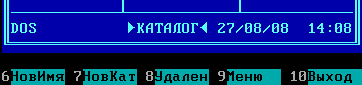
\includegraphics[width=0.5\textwidth]{patterns/01_helloworld/Norton_Commander_v5_51.png}
\caption{\ITph{}}
\end{figure}

Probabilmente questo è successo in molti Paesi durante quel periodo.


\subsection{x86-64}
\EN{\subsubsection{MSVC: x86-64}

\myindex{x86-64}
Let's also try 64-bit MSVC:

\lstinputlisting[caption=MSVC 2012 x64,style=customasmx86]{patterns/01_helloworld/MSVC_x64.asm}

\myindex{fastcall}

In x86-64, all registers were extended to 64-bit, and now their names have an \TT{R-} prefix.
In order to use the stack less often (in other words, to access external memory/cache less often), there is
a popular way to pass function arguments via registers (\emph{fastcall}) \myref{fastcall}.
I.e., a part of the function's arguments are passed in registers, and the rest---via the stack.
In Win64, 4 function arguments are passed in the \RCX, \RDX, \Reg{8}, and \Reg{9} registers.
That is what we see here: a pointer to the string for \printf is now passed not in the stack, but rather in the \RCX register.
The pointers are 64-bit now, so they are passed in the 64-bit registers (which have the \TT{R-} prefix).
However, for backward compatibility, it is still possible to access the 32-bit parts, using the \TT{E-} prefix.
This is how the \RAX/\EAX/\AX/\AL register looks like in x86-64:

\RegTableOne{RAX}{EAX}{AX}{AH}{AL}

The \main function returns an \Tint{}-typed value, which in \CCpp is still 32-bit, for better backward compatibility
and portability, so that is why the \EAX register is cleared at the function end (i.e., the 32-bit
part of the register) instead of with \RAX{}.
There are also 40 bytes allocated in the local stack.
This is called the \q{shadow space}, which we'll talk about later: \myref{shadow_space}.
}
\FR{\subsubsection{MSVC: x86-64}

\myindex{x86-64}
Essayons MSVC 64-bit:

\lstinputlisting[caption=MSVC 2012 x64,style=customasmx86]{patterns/01_helloworld/MSVC_x64.asm}

\myindex{fastcall}

En x86-64, tous les registres ont été étendus à 64-bit et leurs noms ont maintenant le préfixe \TT{R-}.
Afin d'utiliser la pile moins souvent (en d'autres termes, pour accéder moins souvent à la mémoire externe/au cache),
il existe un moyen répandu de passer les arguments aux fonctions par les registres (\emph{fastcall}) \myref{fastcall}.
I.e., une partie des arguments de la fonction est passée par les registres, le reste---par la pile.
En Win64, 4 arguments de fonction sont passés dans les registres \RCX, \RDX, \Reg{8}, \Reg{9}.
C'est ce que l'on voit ci-dessus: un pointeur sur la chaîne pour \printf est passé non pas par la pile,
mais par le registre \RCX.
Les pointeurs font maintenant 64-bit, ils sont donc passés dans les registres 64-bit (qui ont le préfixe \TT{R-}).
Toutefois, pour la rétrocompatibilité, il est toujours possible d'accéder à la partie 32-bits des registres,
en utilisant le préfixe \TT{E-}.
Voici à quoi ressemblent les registres \RAX/\EAX/\AX/\AL en x86-64:

\RegTableOne{RAX}{EAX}{AX}{AH}{AL}

La fonction \main renvoie un type \Tint{}, qui est, en \CCpp, pour une meilleure rétrocompatibilité
et portabilité, toujours 32-bit, c'est pourquoi le registre \EAX est mis à zéro à la fin de la fonction (i.e., la
partie 32-bit du registre) au lieu de \RAX{}.
Il y aussi 40 octets alloués sur la pile locale.
Cela est appelé le \q{shadow space}, dont nous parlerons plus tard: \myref{shadow_space}.
}
\IT{\subsubsection{MSVC: x86-64}

\myindex{x86-64}
Proviamo anche con MSVC a 64-bit:

\lstinputlisting[caption=MSVC 2012 x64,style=customasmx86]{patterns/01_helloworld/MSVC_x64.asm}

\myindex{fastcall}

In x86-64, tutti i registri sono stati estesi a 64-bit ed il loro nome ha il prefisso \TT{R-}.
Per usare lo stack meno spesso (in altre parole, per accedere meno spesso alla memoria esterna/cache), esiste un metodo molto diffuso per passare gli argomenti delle funzioni tramite i registri (\emph{fastcall})
\myref{fastcall}.
Ovvero, una parte degli argomenti viene passata attraverso i registri, il resto ---attraverso lo stack.
In Win64, 4 argomenti di funzione sono passati nei registri \RCX, \RDX, \Reg{8}, \Reg{9}.
Questo è ciò che vediamo qui: un puntatore alla stringa per \printf è adesso passato nel registro \RCX anziché tramite lo stack.
I puntatori adesso sono a 64-bit, quindi vengono passati nei registri a 64-bit (aventi il prefisso \TT{R-}).
E' comunque possibile, per retrocompatibilità, accedere alle parti a 32-bit, usando il prefisso \TT{E-}.
I registri \RAX/\EAX/\AX/\AL in x86-64 appaiono così:

\RegTableOne{RAX}{EAX}{AX}{AH}{AL}

La funzione \main restituisce un valore di tipo \Tint{}, che in \CCpp, per migliore retrocompatibilità e portabilità, resta ancora a 32-bit, motivo per cui il registro \EAX (quindi la parte a 32 bit del registro) viene svuotato invece di \RAX{} alla fine della funzione.
Ci sono anche 40 byte allocati nello stack locale.
Questo spazio è detto \q{shadow space}, e ne parleremo più avanti: \myref{shadow_space}.
}
\NL{\subsubsection{MSVC: x86-64}

\myindex{x86-64}
Laat ons ook eens kijken naar 64-bit MSVC:

\lstinputlisting[caption=MSVC 2012 x64,style=customasmx86]{patterns/01_helloworld/MSVC_x64.asm}

\myindex{fastcall}

In x86-64 zijn alle registers uitgebreid tot 64-bit, en hebben hun namen een \TT{R-} prefix gekregen.
Om de stack minder te gebruiken (met andere woorden, om het externe geheugen/cache minder vaak te benaderen), bestaat
er een populaire manier om functies parameters door te geven via registers (\emph{fastcall}) \myref{fastcall}.
Bv., een deel van de parameters wordt doorgegeven via het register, de rest --- via de stack.
In Win64, worden 4 functie parameters doorgegeven via de \RCX, \RDX, \Reg{8}, \Reg{9} registers.
Dat is wat we hier zien: een pointer naar de string voor \printf wordt doorgegeven, niet via de stack, maar via het \RCX register.
De pointers zijn 64-bit nu, dus worden ze doorgegeven in de 64-bit registers (dewelke de \TT{R-} prefix hebben).
Voor backward compatibility is het echter nog steeds mogelijk om de 32-bit gedeelten aan te spreken, door gebruik te maken van de \TT{E-} prefix.
Dit is hoe de \RAX/\EAX/\AX/\AL registers eruit zien in x86-64:

\RegTableOne{RAX}{EAX}{AX}{AH}{AL}

De \main functie geeft een \Tint{}-typed waarde terug, hetwelk, in \CCpp, voor betere backward compatibiliteit
en portabiliteit, nog steeds 32-bit is. Daarom wordt het \EAX register ook leeggemaakt bij het einde van de functie
(het 32-bit gedeelte van het register) in plaats van \RAX{}.
Er zijn ook 40 bytes gealloceerd op de lokale stack.
Dit wordt de \q{shadow space} genoemd, waarover we het later nog gaan hebben: \myref{shadow_space}.

}
\RU{\subsubsection{MSVC: x86-64}

\myindex{x86-64}
Попробуем также 64-битный MSVC:

\lstinputlisting[caption=MSVC 2012 x64,style=customasmx86]{patterns/01_helloworld/MSVC_x64.asm}

\myindex{fastcall}

В x86-64 все регистры были расширены до 64-х бит и теперь имеют префикс \TT{R-}.
Чтобы поменьше задействовать стек (иными словами, поменьше обращаться к кэшу и внешней памяти), уже давно имелся
довольно популярный метод передачи аргументов функции через регистры (\emph{fastcall}) \myref{fastcall}.
Т.е. часть аргументов функции передается через регистры и часть ---через стек.
В Win64 первые 4 аргумента функции передаются через регистры \RCX, \RDX, \Reg{8}, \Reg{9}.
Это мы здесь и видим: указатель на строку в \printf теперь передается не через стек, а через регистр \RCX.
Указатели теперь 64-битные, так что они передаются через 64-битные части регистров (имеющие префикс \TT{R-}).
Но для обратной совместимости можно обращаться и к нижним 32 битам регистров используя префикс \TT{E-}.
Вот как выглядит регистр \RAX/\EAX/\AX/\AL в x86-64:

\RegTableOne{RAX}{EAX}{AX}{AH}{AL}

Функция \main возвращает значение типа \Tint, который в \CCpp, надо полагать, для лучшей совместимости и переносимости,
оставили 32-битным. Вот почему в конце функции \main обнуляется не \RAX, а \EAX, т.е. 32-битная часть регистра.
Также видно, что 40 байт выделяются в локальном стеке.
Это \q{shadow space} которое мы будем рассматривать позже: \myref{shadow_space}.
}
\PTBR{\subsubsection{MSVC: x86-64}

\myindex{x86-64}
Vamos tentar também o MSVC 64-bits:

\lstinputlisting[caption=MSVC 2012 x64,style=customasmx86]{patterns/01_helloworld/MSVC_x64.asm}

\myindex{fastcall}

No x86-64, todos os registradores foram extendidos para 64-bits e agora seus nomes contém um \TT{R-} no prefixo.
A fim de diminuir a frequência com que a stack (pilha) é usada (em outras palavras, para acessar memória externa/cache menos vezes),
existe uma maneira popular de passar argumentos para funções através dos registradores (\emph{fastcall}) \myref{fastcall}.
Por exemplo, uma parte dos argumentos da função é passada nos registradores, o resto pela stack.
No Win64, 4 argumentos de funções são passados através dos registradores \RCX, \RDX, \Reg{8}, \Reg{9}.
Que é o que nós vemos, um ponteiro para a string para o printf() não é passado pela stack, mas no registrador \RCX.
Os ponteiros são 64-bits agora, então, eles são passados através dos registradores de 64-bits (que tem prefixo \TT{R-}).
Entretanto, para compatibilidade, ainda é possível acessar partes de 32-bits, usando o prefixo \TT{E-}.
É assim que os registradores \RAX/\EAX/\AX/\AL se parecem no x86-64:

\RegTableOne{RAX}{EAX}{AX}{AH}{AL}

A função \main retorna um valor do tipo inteiro, que em \CCpp é melhor para compatibilidade com versões anteriores e portabilidade,
de 32-bits, por isso o registrador \EAX é limpo no final da função (a parte de 32-bits do registrador) ao invés de \RAX.
Há também 40 bytes alocados na pilha local.
Que é chamado de ``shadow space'', o qual falaremos mais tarde: \myref{shadow_space}.

}
\DE{\subsubsection{MSVC: x86-64}

\myindex{x86-64}
Hier das gleiche Beispiel mit der 64-Bit-Variante von MSVC kompiliert:

\lstinputlisting[caption=MSVC 2012 x64,style=customasmx86]{patterns/01_helloworld/MSVC_x64.asm}

\myindex{fastcall}

In x86-64 wurden alle Regeister auf 64-Bit erweitert und die Registernamen mit einem \TT{R-}Prefix versehen.
Um den Stack weniger oft zu nutzen (also um auf externen Speicher / Cache selterner zuzugreifen), existiert
ein verbreiteter Weg um Funktionsargumente per Register (\emph{fastcall}) \myref{fastcall} zu übergeben.
Das heißt ein Teil der Funktionsargumente wird in Registern übergeben, der Rest---über den Stack.
In Win64 werden vier Funktionsargumente in den Registern \RCX, \RDX, \Reg{8} und \Reg{9} übergeben.
Das ist was hier sichtbar ist: der Zeiger zu der Zeichenkette für \printf ist jetzt nicht im Stack übergeben sondern im \RCX-Register.
Die Zeiger sind nun 64-Bit breit, also werden sie in den 64-Bit-Registern übergeben (die jetz den \TT{R-}Prefix haben).
Aus Gründen der Rückwärtskompatibilität ist es aber immer noch möglich mit dem \TT{E-}Prefix auf 32-Bit-Teile zuzugrifen.
Nachfolgend, der Aufbau der \RAX/\EAX/\AX/\AL-Register in x86-64:

\RegTableOne{RAX}{EAX}{AX}{AH}{AL}

Die \main-Funktion gibt einen Wert vom Typ \Tint{} zurück, der in \CCpp aus Gründen der Kompatibilität und
Portabilität immernoch 32 Bit breit ist. Daher wird am Ende der Funktion das \EAX-Register auf Null gesetzt
(das heißt der 32-Bit-Part des Registers) anstatt \RAX{}.
Auf dem lokalen Stack sind zusätzliche 40 Byte reserviert.
Dieser Bereich wird \q{shadow space} genannt und wird in Abschnitt \myref{shadow_space} noch genauer betrachtet.
}
\PL{\subsubsection{MSVC: x86-64}

\myindex{x86-64}
Wypróbujmy również 64-bitowy MSVC:

\lstinputlisting[caption=MSVC 2012 x64,style=customasmx86]{patterns/01_helloworld/MSVC_x64.asm}

\myindex{fastcall}

W x86-64 wszystkie rejestry zostały rozszerzone do 64-ch bit i mają teraz prefiks \TT{R-}.
Żeby jak najrzadziej korzystać ze stosu (inaczej mówiąc, jak najmniej korzystać z pamięci cache i pamięci zewnętrznej), od dawna istniała dosyć popularna metoda przekazywania argumentów funkcji przez rejestry (\emph{fastcall}) \myref{fastcall}.
Tzn część argumentów funkcji jest przekazywana przez rejestry i część --- przez stos.
W Win64 pierwsze 4 argumenty funkcji są przekazywane przez rejestry \RCX, \RDX, \Reg{8}, \Reg{9}.
Właśnie to tutaj widzimy: wskaźnik na linię \printf teraz jest przekazywany nie przez stos, a przez rejestr \RCX.
Wskaźniki teraz są 64-bitowe, także są one przekazywane przez 64-bitowe części rejestrów (mające prefiks \TT{R-}).
Ale dla wstecznej kompatybilności można adresować również młodsze 32 bity rejestrów poprzez prefiks \TT{E-}.
W ten o to sposób wygląda rejestr \RAX/\EAX/\AX/\AL w x86-64:

\RegTableOne{RAX}{EAX}{AX}{AH}{AL}

Funkcja \main zwraca wartość typu \Tint, który w \CCpp, dla większej kompatybilności,
zostawili 32-bitowym. Właśnie dlatego na końcu f-cji \main zeruje się nie \RAX, a \EAX, czyli 32-bitowa część rejestru.
Także widać, że 40 bajt są przydzielane na stosie lokalnym.
Jest to \q{shadow space} które będzie omawiane później: \myref{shadow_space}.

}
\JA{\subsubsection{MSVC: x86-64}

\myindex{x86-64}
64ビットのMSVCも試してみましょう。

\lstinputlisting[caption=MSVC 2012 x64,style=customasmx86]{patterns/01_helloworld/MSVC_x64.asm}

\myindex{fastcall}

x86-64では、すべてのレジスタが64ビットに拡張されましたが、その名前には\TT{R-}プレフィックスが付いています。 
スタックをあまり頻繁に使用しないように(言い換えると、外部メモリ/キャッシュにアクセスする頻度を減らす)、
レジスタ(\emph{fastcall}) \myref{fastcall}を介して関数引数を渡す一般的な方法があります。 
すなわち、関数の引数の一部はレジスタに渡され、残りはスタックに渡されます。 
Win64では、4つの関数引数が \RCX 、 \RDX 、 \Reg{8} 、および \Reg{9} レジスタに渡されます。 
ここで見るものは: \printf の文字列へのポインタはスタックにではなく、 \RCX レジスタに渡されます。 
ポインタは現在64ビットであるため、64ビットレジスタ(\TT{R-}プレフィックスを持つ)に渡されます。 
ただし、下位互換性を保つために、\TT{E-}接頭辞を使用して32ビットのパーツにアクセスすることは可能です。 
これは、 \RAX/\EAX/\AX/\AL レジスタがx86-64のように見える方法です。

\RegTableOne{RAX}{EAX}{AX}{AH}{AL}

\main 関数は\Tint{}型の値を返します。これは \CCpp では32ビットのままで、下位互換性と移植性を向上させるため、
関数終了時に \RAX レジスタの代わりに \EAX レジスタがクリアされる理由です。(すなわちレジスタの32ビットの部分) 
ローカルスタックには40バイトも割り当てられています。 
これは\q{シャドースペース}と呼ばれます。これについては後で説明します:\myref{shadow_space}
}

\EN{\input{patterns/01_helloworld/GCC_x64_EN}}
\FR{\input{patterns/01_helloworld/GCC_x64_FR}}
\RU{\input{patterns/01_helloworld/GCC_x64_RU}}
\NL{\input{patterns/01_helloworld/GCC_x64_NL}}
\IT{\subsubsection{GCC: x86-64}

\myindex{x86-64}
Proviamo anche GCC in Linux a 64-bit:

\lstinputlisting[caption=GCC 4.4.6 x64,,style=customasmx86]{patterns/01_helloworld/GCC_x64_EN.s}

% I think I got the intent right on the following line - Renaissance
Linux, *BSD e \MacOSX usano anche un metodo per passare argomenti di funzione nei registri. \SysVABI.

I primi 6 argomenti sono passati nei registri \RDI, \RSI, \RDX, \RCX, \Reg{8}, \Reg{9}, ed il resto---tramite lo stack.

Quindi il puntatore alla stringa viene passato in \EDI (la parte a 32-bit del registro).
Ma perchè non utilizza la parte a 64-bit, \RDI?

E' importante ricordare che tutte le istruzioni \MOV in modalità 64-bit che scrivono qualcosa nella parte dei 32-bit bassa di un registro, azzera anche la parte a 32-bit alta (come indicato nei manuali Intel: \myref{x86_manuals}).\\
Ad esempio, \INS{MOV EAX, 011223344h} scrive correttamente un valore in \RAX, poichè i bit della parte alta verranno azzerati.

Se apriamo il file oggetto compilato (.o), possiamo anche vedere gli opcode di tutte le istruzioni
\footnote{Questo deve essere abilitato in \textbf{Options $\rightarrow$ Disassembly $\rightarrow$ Number of opcode bytes}}:

\lstinputlisting[caption=GCC 4.4.6 x64,style=customasmx86]{patterns/01_helloworld/GCC_x64.lst}

\label{hw_EDI_instead_of_RDI}
Come possiamo notare, l'istruzione che scrive in \EDI all'indirizzo \TT{0x4004D4} occupa 5 byte.
La stessa istruzione che scrive un valore a 64-bit in \RDI occupa 7 bytes.
Apparentemente, GCC sta cercando di risparmiare un po' di spazio.
Inoltre, può essere sicuro che il segmento dati contenente la stringa non sarà allocato ad indirizzi maggiori di 4\gls{GiB}.

\label{SysVABI_input_EAX}
% There isn't an ABI acronym in acronyms.tex - I figure the intent is to Application Binary Interface,
% so I put it in there (in the EN section, commented out)
Notiamo anche che il registro \EAX è stato azzerato prima della chiamata alla funzione \printf.
Questo viene fatto perché, in base allo standard \ac{ABI} citato in precedenza,
il numero dei registri vettore usati deve essere passato in \EAX nei sistemi *NIX su x86-64.
}
\DE{\input{patterns/01_helloworld/GCC_x64_DE}}
\PL{\input{patterns/01_helloworld/GCC_x64_PL}}
\JPN{\input{patterns/01_helloworld/GCC_x64_JPN}}

\subsubsection{Address patching (Win64)}

Se il nostro esempio venisse compilato in MSVC 2013 utilizzando lo switch \TT{\textbackslash{}MD}
(che significa un eseguibile più piccolo a causa del link dei file \TT{MSVCR*.DLL}), la funzione \main verrebbe prima, e può essere trovata facilmente:

\begin{figure}[H]
\centering
\myincludegraphics{patterns/01_helloworld/hiew_incr1.png}
\caption{Hiew}
\label{}
\end{figure}

Come esperimento, possiamo \glslink{increment}{incrementare} l'indirizzo di 1:

\begin{figure}[H]
\centering
\myincludegraphics{patterns/01_helloworld/hiew_incr2.png}
\caption{Hiew}
\label{}
\end{figure}

Hiew mostra \q{ello, world}.
E quando lanciamo l'eseguibile modificato, viene stampata proprio questa stringa.

\subsubsection{Scegliere un'altra stringa dall'immagine binaria (Linux x64)}

Il file binario che si ottiene compilando il nostro esempio tramite GCC 5.4.0 su Linux x64 contiene molte altre stringhe di testo.
Si tratta principalmente di nomi di funzioni e librerie importate.

Esegui objdump per ottenere il contenuto di tutte le sezioni del file compilato:

\begin{lstlisting}[basicstyle=\ttfamily, mathescape]
$\$$ objdump -s a.out

a.out:     file format elf64-x86-64

Contents of section .interp:
 400238 2f6c6962 36342f6c 642d6c69 6e75782d  /lib64/ld-linux-
 400248 7838362d 36342e73 6f2e3200           x86-64.so.2.
Contents of section .note.ABI-tag:
 400254 04000000 10000000 01000000 474e5500  ............GNU.
 400264 00000000 02000000 06000000 20000000  ............ ...
Contents of section .note.gnu.build-id:
 400274 04000000 14000000 03000000 474e5500  ............GNU.
 400284 fe461178 5bb710b4 bbf2aca8 5ec1ec10  .F.x[.......^...
 400294 cf3f7ae4                             .?z.

...
\end{lstlisting}

Non è un problema passare l'indirizzo della stringa di test \q{/lib64/ld-linux-x86-64.so.2} a \TT{printf()}:

\begin{lstlisting}[style=customc]
#include <stdio.h>

int main()
{
    printf(0x400238);
    return 0;
}
\end{lstlisting}

E' difficile da credere, ma questo codice stampa la stringa citata prima.

Se cambiassi l'indirizzo a \TT{0x400260}, verrebbe stampata la stringa \q{GNU}.
Questo indirizzo è corretto per la mia specifica versione di GCC, GNU toolset, etc.
Sul tuo sistema, l'eseguibile potrebbe essere leggermente differente, e anche tutti gli indirizzi sarebbero differenti.
Inoltre, aggiungendo o rimuovendo del codice in/da questo codice sorgente probabilmente sposterebbe tutti gli indirizzi in avanti o indietro.


\EN{\subsection{GCC---one more thing}
\label{use_parts_of_C_strings}

The fact that an \IT{anonymous} C-string has \IT{const} type (\myref{string_is_const_char}), 
and that C-strings allocated in constants segment are guaranteed to be immutable, has an interesting consequence:
the compiler may use a specific part of the string.

Let's try this example:

\begin{lstlisting}[style=customc]
#include <stdio.h>

int f1()
{
	printf ("world\n");
}

int f2()
{
	printf ("hello world\n");
}

int main()
{
	f1();
	f2();
}
\end{lstlisting}

Common \CCpp{}-compilers (including MSVC) allocate two strings, but let's see what GCC 4.8.1 does:

\lstinputlisting[caption=GCC 4.8.1 + IDA listing,style=customasmx86]{patterns/01_helloworld/two_strings.asm}

Indeed: when we print the \q{hello world} string
these two words are positioned in memory adjacently and \puts called from \GTT{f2()}
function is not aware that this string is divided. 
In fact, it's not divided; it's divided only \q{virtually}, in this listing.

When \puts is called from \GTT{f1()}, it uses the \q{world} string plus a zero byte. \puts is not aware that there is something before this string!

This clever trick is often used by at least GCC and can save some memory.
This is close to \IT{string interning}.

Another related example is here: \myref{strstr_example}.

}
\FR{\subsection{GCC---encore une chose}
\label{use_parts_of_C_strings}

Le fait est qu'une chaîne C \emph{anonyme} a un type \emph{const} (\myref{string_is_const_char}),
et que les chaînes C allouées dans le segment des constantes sont garanties d'être immuables,
a cette conséquence intéressante:
Le compilateur peut utiliser une partie spécifique de la chaîne.

Voyons cela avec un exemple:

\begin{lstlisting}[style=customc]
#include <stdio.h>

int f1()
{
	printf ("world\n");
}

int f2()
{
	printf ("hello world\n");
}

int main()
{
	f1();
	f2();
}
\end{lstlisting}

La plupart des compilateurs \CCpp{} (MSVC inclus) allouent deux chaînes, mais voyons ce que fait GCC 4.8.1:

\lstinputlisting[caption=GCC 4.8.1 + IDA,style=customasmx86]{patterns/01_helloworld/two_strings.asm}

Effectivement: lorsque nous affichons la chaîne \q{hello world} ses deux mots sont positionnés
consécutivement en mémoire et l'appel à \puts depuis la fonction \GTT{f2()}
n'est pas au courant que la chaîne est divisée.
En fait, elle n'est pas divisée; elle l'est \q{virtuellement}, dans ce listing.

Lorsque \puts est appelé depuis \GTT{f1()}, il utilise la chaîne \q{world} ainsi qu'un
octet à zéro. \puts ne sait pas qu'il y a quelque chose avant cette chaîne!

Cette astuce est souvent utilisée, au moins par GCC, et permet d'économiser de la mémoire.
C'est proche du \emph{string interning}. % TODO clarify imbrication de chaînes ?

Un autre exemple concernant ceci se trouve là: \myref{strstr_example}.

}
\IT{\subsection{GCC---un'altra cosa}
\label{use_parts_of_C_strings}

Il fatto che una stringa C \emph{anonima} abbia tipo \emph{const} (\myref{string_is_const_char}),
e che le stringhe C allocate in in segmenti costanti siano garantite come immutabili, ha una conseguenza interessante:
il compilatore può utilizzare una parte specifica della stringa.

Proviamo questo esempio:

\begin{lstlisting}[style=customc]
#include <stdio.h>

int f1()
{
	printf ("world\n");
}

int f2()
{
	printf ("hello world\n");
}

int main()
{
	f1();
	f2();
}
\end{lstlisting}

Compilatori \CCpp{} comuni (incluso MSVC) allocano due stringhe, ma vediamo cosa fa GCC 4.8.1:

\lstinputlisting[caption=GCC 4.8.1 + IDA,style=customasmx86]{patterns/01_helloworld/two_strings.asm}

Infatti: quando stampiamo la stringa \q{hello world}
queste due parole sono memorizzate in posizioni adiacenti in memoria e \puts chiamata dalla funzione \GTT{f2()}
non sa che questa stringa è divisa.
In effett, non è veramente divisa; è separata solo \q{virtualmente}, in questo listato.

Quando \puts viene chiamato da \GTT{f1()}, usa la stringa \q{world} più un byte zero. \puts che è presente qualcosa prima di questa stringa!

Questo trucchetto furbo viene utilizzato perlomeno da GCC e può salvare un po' di memoria.
Questo è simile allo \emph{string interning}.

Un ulteriore esempio correlato è questo: \myref{strstr_example}.
}
\NL{% TODO to be resynced with English version
\subsection{GCC---Nog een ding}
\label{use_parts_of_C_strings}

Het feit dat een \IT{anonieme} C-string het type \IT{const} heeft (\myref{string_is_const_char}), 
en dat C-string gealloceerd in het segment met de constanten gegarandeerd immuteerbaar zijn, heeft een interessant gevolg:
De compiler kan een specifiek gedeelte van de string gebruiken.

Laten we dit voorbeeld proberen:

\begin{lstlisting}[style=customc]
#include <stdio.h>

int f1()
{
	printf ("world\n");
}

int f2()
{
	printf ("hello world\n");
}

int main()
{
	f1();
	f2();
}
\end{lstlisting}

Veelgebruikte \CCpp{}-compilers (inclusief MSVC) alloceren twee strings, maar laat ons eens kijken wat GCC 4.8.1 doet:

\lstinputlisting[caption=GCC 4.8.1 + IDA,style=customasmx86]{patterns/01_helloworld/two_strings.asm}

Inderdaad: wanneer we de \q{hello world} string printen, 
Worden deze twee woorden aangrenzend in het geheugen geplaatsd, en \puts, die geroepen wordt van de \GTT{f2()}
functie, is er zicht niet van bewust dat deze string opgedeeld is. 
In feite is hij ook niet opgedeeld, hij is slechts \q{virtueel} opgedeeld in deze listing.

Wanneer \puts aangeroepen wordt vanuit \GTT{f1()}, gebruikt het de \q{world} string plus een nulbyte. \puts is er zich niet van bewust dat er nog iets voor deze string staat!

Dit slimme truukje wordt vaak gebruikt door op zijn minst GCC, en kan geheugen besparen.

}
\RU{\subsection{GCC --- ещё кое-что}
\label{use_parts_of_C_strings}

Тот факт, что \IT{анонимная} Си-строка имеет тип \IT{const} (\myref{string_is_const_char}), 
и тот факт, что выделенные в сегменте констант Си-строки гарантировано неизменяемые (immutable), 
ведет к интересному следствию: компилятор может использовать определенную часть строки.

Вот простой пример:

\begin{lstlisting}[style=customc]

#include <stdio.h>

int f1()
{
	printf ("world\n");
}

int f2()
{
	printf ("hello world\n");
}

int main()
{
	f1();
	f2();
}
\end{lstlisting}

Среднестатистический компилятор с \CCpp (включая MSVC) выделит место для двух строк, но вот что делает GCC 4.8.1:

\lstinputlisting[caption=GCC 4.8.1 + листинг в IDA,style=customasmx86]{patterns/01_helloworld/two_strings.asm}

Действительно, когда мы выводим строку \q{hello world}, 
эти два слова расположены в памяти впритык друг к другу и \puts, вызываясь из функции \GTT{f2()}, вообще не знает,
что эти строки разделены. Они и не разделены на самом деле, они разделены
только \q{виртуально}, в нашем листинге.

Когда \puts вызывается из \GTT{f1()}, он использует строку \q{world} плюс нулевой байт. \puts не знает, что там ещё есть какая-то строка перед этой!

Этот трюк часто используется (по крайней мере в GCC) и может сэкономить немного памяти.
Это близко к \IT{string interning}.

Еще один связанный с этим пример находится здесь: \myref{strstr_example}.

}
\DE{% TODO to be resynced with EN version
\subsection{GCC---eine weitere Sache}
\label{use_parts_of_C_strings}

Die Tatsache, dass eine \emph{anonyme} C-Zeichenkette den Typ \emph{const} hat (\myref{string_is_const_char}), 
und dass C-Zeichenketten im Segment für konstante Daten angelegt sind (was dafür sorgt, dass sie unveränderbar sind),
hat eine interessante Auswirkung: der Compiler kann spezifische Teile der Zeichenkette verwenden.

Probieren wir das folgende Beispiel:

\begin{lstlisting}[style=customc]
#include <stdio.h>

int f1()
{
	printf ("world\n");
}

int f2()
{
	printf ("hello world\n");
}

int main()
{
	f1();
	f2();
}
\end{lstlisting}

Gebräuchliche \CCpp{}-Compiler (inklusive MSVC) allozieren zwei Strings.
Im Folgenden jedoch ist abgebildet, was GCC 4.8.1 erzeugt:

\lstinputlisting[caption=GCC 4.8.1 + IDA,style=customasmx86]{patterns/01_helloworld/two_strings.asm}

Wenn die Zeichenkette \q{hello world} ausgegeben wird, werden die beiden Worte im Speicher nebeneinander
positioniert und die Funktion \puts in \GTT{f2()} merkt nicht, dass die Zeichenkette geteilt ist.
Tatsächlich ist sie lediglich \q{virtuell} in diesem Listing geteilt.

Wenn \puts aus der Funktion \GTT{f1()} aufgerufen wird, wir die \q{world}-Zeichenkette plus einem Null-Byte
genutzt. \puts merkt nicht, dass sich davor noch etwas befindet.

Dieser clevere Trick wird von GCC oft genutzt und ermöglicht das Einsparen von etwas Speicher.

Ein weiteres Beispiel ist hier: \myref{strstr_example}.

}
\PL{\subsection{GCC --- jeszcze co nieco}
\label{use_parts_of_C_strings}

To, że \emph{anonimowa} linia w C ma typ \emph{const} (\myref{string_is_const_char}), 
i to, że zaznaczone w segmencie stałych C-linie są gwarantowanie nie do zmiany (immutable), 
prowadzi do ciekawych konsekwencji: kompilator może korzystać tylko z pewnej części linii.

Prosty przykład:

\begin{lstlisting}[style=customc]

#include <stdio.h>

int f1()
{
	printf ("world\n");
}

int f2()
{
	printf ("hello world\n");
}

int main()
{
	f1();
	f2();
}
\end{lstlisting}

Typowy kompilator \CCpp (w tym MSVC) przydzieli miejsce dla 2 linii, ale oto jest to co robi GCC 4.8.1:

\lstinputlisting[caption=GCC 4.8.1 + listing w IDA,style=customasmx86]{patterns/01_helloworld/two_strings.asm}

Naprawdę, kiedy printujemy linię \q{hello world}, 
te dwa słowa są usytuowane w pamięci tuż obok siebie i \puts, będąc wywołane z funkcji \GTT{f2()}, w ogóle nie wie,
że te linię są rozdzielone. Tak naprawdę to one i nie są rozdzielone, są rozdzielone 
tylko \q{wirtualnie}, w naszym listingu.

Kiedy \puts zostaje wywołane z \GTT{f1()}, ono wykorzystuje linię \q{world} + zerowy bajt. \puts w ogóle nie wie, że tam jest jeszcze jakaś linia przed tą!

Ten trik jest często wykorzystywany (przynajmniej w GCC) i może zaoszczędzić trochę pamięci.
Jest to podobny mechanizm do mechanizmu \emph{internowania łańcuchów}.

Jeszcze jeden przykład można znaleźć tutaj: \myref{strstr_example}.


}
\JPN{\subsection{GCC---もう1つ}
\label{use_parts_of_C_strings}

\emph{匿名の}C文字列が\emph{const}型(\myref{string_is_const_char})を持ち、
定数セグメントに割り当てられたC文字列が不変であることが保証されているという事実は興味深い結果をもたらします:
コンパイラは文字列の特定の部分を使用するかもしれません。

下記の例で試してみましょう。

\begin{lstlisting}[style=customc]
#include <stdio.h>

int f1()
{
	printf ("world\n");
}

int f2()
{
	printf ("hello world\n");
}

int main()
{
	f1();
	f2();
}
\end{lstlisting}

一般的な \CCpp{} コンパイラ(MSVCを含む)は2つの文字列を割り当てますが、GCC 4.8.1の動作を見てみましょう。

\lstinputlisting[caption=GCC 4.8.1 + IDA,style=customasmx86]{patterns/01_helloworld/two_strings.asm}

確かに、\q{hello world}という文字列を印刷すると、これらの2つの単語はメモリに隣接して配置され、\GTT{f2()}関数から呼び出される \puts 関数はこの文字列が分割されていることを認識しません。 
実際、分割されていません。 このリストには、\q{仮想的に}分けられています。

\puts が\GTT{f1()}から呼び出されると、\q{world}文字列とNULLバイトを使用します。 \puts はこの文字列の前に何かがあることを認識していません!

この巧妙なトリックは、少なくともGCCでよく使用され、メモリを節約できます。 これは\emph{文字列インターン}に似ています。

別の関連する例がここにあります:\myref{strstr_example}
}


\EN{\mysection{\MinesweeperWinXPExampleChapterName}
\label{minesweeper_winxp}
\myindex{Windows!Windows XP}

For those who are not very good at playing Minesweeper, we could try to reveal the hidden mines in the debugger.

\myindex{\CStandardLibrary!rand()}
\myindex{Windows!PDB}

As we know, Minesweeper places mines randomly, so there has to be some kind of random number generator or
a call to the standard \TT{rand()} C-function.

What is really cool about reversing Microsoft products is that there are \gls{PDB} 
file with symbols (function names, \etc{}).
When we load \TT{winmine.exe} into \IDA, it downloads the 
\gls{PDB} file exactly for this 
executable and shows all names.

So here it is, the only call to \TT{rand()} is this function:

\lstinputlisting[style=customasmx86]{examples/minesweeper/tmp1.lst}

\IDA named it so, and it was the name given to it by Minesweeper's developers.

The function is very simple:

\begin{lstlisting}[style=customc]
int Rnd(int limit)
{
    return rand() % limit;
};
\end{lstlisting}

(There is no \q{limit} name in the \gls{PDB} file; we manually named this argument like this.)

So it returns 
a random value from 0 to a specified limit.

\TT{Rnd()} is called only from one place, 
a function called \TT{StartGame()}, 
and as it seems, this is exactly 
the code which place the mines:

\begin{lstlisting}[style=customasmx86]
.text:010036C7                 push    _xBoxMac
.text:010036CD                 call    _Rnd@4          ; Rnd(x)
.text:010036D2                 push    _yBoxMac
.text:010036D8                 mov     esi, eax
.text:010036DA                 inc     esi
.text:010036DB                 call    _Rnd@4          ; Rnd(x)
.text:010036E0                 inc     eax
.text:010036E1                 mov     ecx, eax
.text:010036E3                 shl     ecx, 5          ; ECX=ECX*32
.text:010036E6                 test    _rgBlk[ecx+esi], 80h
.text:010036EE                 jnz     short loc_10036C7
.text:010036F0                 shl     eax, 5          ; EAX=EAX*32
.text:010036F3                 lea     eax, _rgBlk[eax+esi]
.text:010036FA                 or      byte ptr [eax], 80h
.text:010036FD                 dec     _cBombStart
.text:01003703                 jnz     short loc_10036C7
\end{lstlisting}

Minesweeper allows you to set the board size, so the X (xBoxMac) and Y (yBoxMac) of the board are global variables.
They are passed to \TT{Rnd()} and random 
coordinates are generated.
A mine is placed by the \TT{OR} instruction at \TT{0x010036FA}. 
And if it has been placed before 
(it's possible if the pair of \TT{Rnd()} 
generates a coordinates pair which has been already 
generated), 
then \TT{TEST} and \TT{JNZ} at \TT{0x010036E6} 
jumps to the generation routine again.

\TT{cBombStart} is the global variable containing total number of mines. So this is loop.

The width of the array is 32 
(we can conclude this by looking at the \TT{SHL} instruction, which multiplies one of the coordinates by 32).

The size of the \TT{rgBlk} 
global array can be easily determined by the difference 
between the \TT{rgBlk} 
label in the data segment and the next known one. 
It is 0x360 (864):

\begin{lstlisting}[style=customasmx86]
.data:01005340 _rgBlk          db 360h dup(?)          ; DATA XREF: MainWndProc(x,x,x,x)+574
.data:01005340                                         ; DisplayBlk(x,x)+23
.data:010056A0 _Preferences    dd ?                    ; DATA XREF: FixMenus()+2
...
\end{lstlisting}

$864/32=27$.

So the array size is $27*32$?
It is close to what we know: when we try to set board size to $100*100$ in Minesweeper settings, it fallbacks to a board of size $24*30$.
So this is the maximal board size here.
And the array has a fixed size for any board size.

So let's see all this in \olly.
We will ran Minesweeper, attaching \olly to it and now we can see the memory dump at the address of the \TT{rgBlk} array (\TT{0x01005340})
\footnote{All addresses here are for Minesweeper for Windows XP SP3 English. 
They may differ for other service packs.}.

So we got this memory dump of the array:

\lstinputlisting[style=customasmx86]{examples/minesweeper/1.lst}

\olly, like any other hexadecimal editor, shows 16 bytes per line.
So each 32-byte array row occupies exactly 2 lines here.

This is beginner level (9*9 board).

There is some square 
structure can be seen visually (0x10 bytes).

We will click \q{Run} in \olly to unfreeze the Minesweeper process, then we'll clicked randomly at the Minesweeper window 
and trapped into mine, but now all mines are visible:

\begin{figure}[H]
\centering
\myincludegraphicsSmall{examples/minesweeper/1.png}
\caption{Mines}
\label{fig:minesweeper1}
\end{figure}

By comparing the mine places and the dump, we can conclude that 0x10 stands for border, 0x0F---empty block, 0x8F---mine.
Perhaps, 0x10 is just a \emph{sentinel value}.

Now we'll add comments and also enclose all 0x8F bytes into square brackets:

\lstinputlisting[style=customasmx86]{examples/minesweeper/2.lst}

Now we'll remove all \emph{border bytes} (0x10) and what's beyond those:

\lstinputlisting[style=customasmx86]{examples/minesweeper/3.lst}

Yes, these are mines, now it can be clearly seen and compared with the screenshot.

\clearpage
What is interesting is that we can modify the array right in \olly.
We can remove all mines by changing all 0x8F bytes by 0x0F, and here is what we'll get in Minesweeper:

\begin{figure}[H]
\centering
\myincludegraphicsSmall{examples/minesweeper/3.png}
\caption{All mines are removed in debugger}
\label{fig:minesweeper3}
\end{figure}

We can also move all of them to the first line: 

\begin{figure}[H]
\centering
\myincludegraphicsSmall{examples/minesweeper/2.png}
\caption{Mines set in debugger}
\label{fig:minesweeper2}
\end{figure}

Well, the debugger is not very convenient for eavesdropping (which is our goal anyway), so we'll write a small utility
to dump the contents of the board:

\lstinputlisting[style=customc]{examples/minesweeper/minesweeper_cheater.c}

Just set the \ac{PID}
\footnote{PID it can be seen in Task Manager 
(enable it in \q{View $\rightarrow$ Select Columns})} 
and the address of the array (\TT{0x01005340} for Windows XP SP3 English) 
and it will dump it
\footnote{The compiled executable is here: 
\href{http://go.yurichev.com/17165}{beginners.re}}.

It attaches itself to a win32 process by \ac{PID} and just reads process memory at the address.

\subsection{Finding grid automatically}

This is kind of nuisance to set address each time when we run our utility.
Also, various Minesweeper versions may have the array on different address.
Knowing the fact that there is always a border (0x10 bytes), we can just find it in memory:

\lstinputlisting[style=customc]{examples/minesweeper/cheater2_fragment.c}

Full source code: \url{https://github.com/DennisYurichev/RE-for-beginners/blob/master/examples/minesweeper/minesweeper_cheater2.c}.

\subsection{\Exercises}

\begin{itemize}

\item 
Why do the \emph{border bytes} (or \emph{sentinel values}) (0x10) exist in the array?

What they are for if they are not visible in Minesweeper's interface?
How could it work without them?

\item 
As it turns out, there are more values possible (for open blocks, for flagged by user, \etc{}).
Try to find the meaning of each one.

\item 
Modify my utility so it can remove all mines or set them in a fixed pattern that you want in the Minesweeper
process currently running.

\end{itemize}
}
\FR{\subsection{MIPS}

\subsubsection{3 arguments}

\myparagraph{GCC 4.4.5 \Optimizing}

La différence principale avec l'exemple \q{\HelloWorldSectionName} est que dans ce cas, \printf est appelée
à la place de \puts et 3 arguments de plus sont passés à travers les registres \$5\dots \$7 (ou \$A0\dots \$A2).
C'est pourquoi ces registres sont préfixés avec A-, ceci sous-entend qu'ils
sont utilisés pour le passage des arguments aux fonctions.

\lstinputlisting[caption=GCC 4.4.5 \Optimizing (\assemblyOutput),style=customasmMIPS]{patterns/03_printf/MIPS/printf3.O3_FR.s}

\lstinputlisting[caption=GCC 4.4.5 \Optimizing (IDA),style=customasmMIPS]{patterns/03_printf/MIPS/printf3.O3.IDA_FR.lst}

\IDA a agrégé la paire d'instructions \INS{LUI} et \INS{ADDIU} en une pseudo instruction \INS{LA}.
C'est pourquoi il n'y a pas d'instruction à l'adresse 0x1C: car \INS{LA} \emph{occupe} 8 octets.

\myparagraph{GCC 4.4.5 \NonOptimizing}

GCC \NonOptimizing est plus verbeux:

\lstinputlisting[caption=GCC 4.4.5 \NonOptimizing (\assemblyOutput),style=customasmMIPS]{patterns/03_printf/MIPS/printf3.O0_FR.s}

\lstinputlisting[caption=GCC 4.4.5 \NonOptimizing (IDA),style=customasmMIPS]{patterns/03_printf/MIPS/printf3.O0.IDA_FR.lst}

\subsubsection{8 arguments}

Utilisons encore l'exemple de la section précédente avec 9 arguments: \myref{example_printf8_x64}.

\lstinputlisting[style=customc]{patterns/03_printf/2.c}

\myparagraph{GCC 4.4.5 \Optimizing}

Seul les 4 premiers arguments sont passés dans les registres \$A0 \dots \$A3,
les autres sont passés par la pile.
\myindex{MIPS!O32}

C'est la convention d'appel O32 (qui est la plus commune dans le monde MIPS).
D'autres conventions d'appel (comme N32) peuvent utiliser les registres à d'autres fins.

\myindex{MIPS!\Instructions!SW}

\INS{SW} est l'abbréviation de \q{Store Word} (depuis un registre vers la mémoire).
En MIPS, il manque une instructions pour stocker une valeur dans la mémoire, donc
une paire d'instruction doit être utilisée à la place (\INS{LI}/\INS{SW}).

\lstinputlisting[caption=GCC 4.4.5 \Optimizing (\assemblyOutput),style=customasmMIPS]{patterns/03_printf/MIPS/printf8.O3_FR.s}

\lstinputlisting[caption=GCC 4.4.5 \Optimizing (IDA),style=customasmMIPS]{patterns/03_printf/MIPS/printf8.O3.IDA_FR.lst}

\myparagraph{GCC 4.4.5 \NonOptimizing}

GCC \NonOptimizing est plus verbeux:

\lstinputlisting[caption=\NonOptimizing GCC 4.4.5 (\assemblyOutput),style=customasmMIPS]{patterns/03_printf/MIPS/printf8.O0_FR.s}

\lstinputlisting[caption=\NonOptimizing GCC 4.4.5 (IDA),style=customasmMIPS]{patterns/03_printf/MIPS/printf8.O0.IDA_FR.lst}

}
\RU{\mysection{Разгон майнера биткоинов Cointerra}
\index{Bitcoin}
\index{BeagleBone}

Был такой майнер биткоинов Cointerra, выглядящий так:

\begin{figure}[H]
\centering
\myincludegraphics{examples/bitcoin_miner/board.jpg}
\caption{Board}
\end{figure}

И была также (возможно утекшая) утилита\footnote{Можно скачать здесь: \url{https://github.com/DennisYurichev/RE-for-beginners/raw/master/examples/bitcoin_miner/files/cointool-overclock}}
которая могла выставлять тактовую частоту платы.
Она запускается на дополнительной плате BeagleBone на ARM с Linux (маленькая плата внизу фотографии).

И у автора (этих строк) однажды спросили, можно ли хакнуть эту утилиту и посмотреть, какие частоты можно выставлять, и какие нет.
И можно ли твикнуть её?

Утилиту нужно запускать так: \TT{./cointool-overclock 0 0 900}, где 900 это частота в МГц.
Если частота слишком большая, утилита выведет ошибку \q{Error with arguments} и закончит работу.

Вот фрагмент кода вокруг ссылки на текстовую строку \q{Error with arguments}:

\begin{lstlisting}[style=customasmARM]

...

.text:0000ABC4         STR      R3, [R11,#var_28]
.text:0000ABC8         MOV      R3, #optind
.text:0000ABD0         LDR      R3, [R3]
.text:0000ABD4         ADD      R3, R3, #1
.text:0000ABD8         MOV      R3, R3,LSL#2
.text:0000ABDC         LDR      R2, [R11,#argv]
.text:0000ABE0         ADD      R3, R2, R3
.text:0000ABE4         LDR      R3, [R3]
.text:0000ABE8         MOV      R0, R3  ; nptr
.text:0000ABEC         MOV      R1, #0  ; endptr
.text:0000ABF0         MOV      R2, #0  ; base
.text:0000ABF4         BL       strtoll
.text:0000ABF8         MOV      R2, R0
.text:0000ABFC         MOV      R3, R1
.text:0000AC00         MOV      R3, R2
.text:0000AC04         STR      R3, [R11,#var_2C]
.text:0000AC08         MOV      R3, #optind
.text:0000AC10         LDR      R3, [R3]
.text:0000AC14         ADD      R3, R3, #2
.text:0000AC18         MOV      R3, R3,LSL#2
.text:0000AC1C         LDR      R2, [R11,#argv]
.text:0000AC20         ADD      R3, R2, R3
.text:0000AC24         LDR      R3, [R3]
.text:0000AC28         MOV      R0, R3  ; nptr
.text:0000AC2C         MOV      R1, #0  ; endptr
.text:0000AC30         MOV      R2, #0  ; base
.text:0000AC34         BL       strtoll
.text:0000AC38         MOV      R2, R0
.text:0000AC3C         MOV      R3, R1
.text:0000AC40         MOV      R3, R2
.text:0000AC44         STR      R3, [R11,#third_argument]
.text:0000AC48         LDR      R3, [R11,#var_28]
.text:0000AC4C         CMP      R3, #0
.text:0000AC50         BLT      errors_with_arguments
.text:0000AC54         LDR      R3, [R11,#var_28]
.text:0000AC58         CMP      R3, #1
.text:0000AC5C         BGT      errors_with_arguments
.text:0000AC60         LDR      R3, [R11,#var_2C]
.text:0000AC64         CMP      R3, #0
.text:0000AC68         BLT      errors_with_arguments
.text:0000AC6C         LDR      R3, [R11,#var_2C]
.text:0000AC70         CMP      R3, #3
.text:0000AC74         BGT      errors_with_arguments
.text:0000AC78         LDR      R3, [R11,#third_argument]
.text:0000AC7C         CMP      R3, #0x31
.text:0000AC80         BLE      errors_with_arguments
.text:0000AC84         LDR      R2, [R11,#third_argument]
.text:0000AC88         MOV      R3, #950
.text:0000AC8C         CMP      R2, R3
.text:0000AC90         BGT      errors_with_arguments
.text:0000AC94         LDR      R2, [R11,#third_argument]
.text:0000AC98         MOV      R3, #0x51EB851F
.text:0000ACA0         SMULL    R1, R3, R3, R2
.text:0000ACA4         MOV      R1, R3,ASR#4
.text:0000ACA8         MOV      R3, R2,ASR#31
.text:0000ACAC         RSB      R3, R3, R1
.text:0000ACB0         MOV      R1, #50
.text:0000ACB4         MUL      R3, R1, R3
.text:0000ACB8         RSB      R3, R3, R2
.text:0000ACBC         CMP      R3, #0
.text:0000ACC0         BEQ      loc_ACEC
.text:0000ACC4
.text:0000ACC4 errors_with_arguments
.text:0000ACC4                                         
.text:0000ACC4         LDR      R3, [R11,#argv]
.text:0000ACC8         LDR      R3, [R3]
.text:0000ACCC         MOV      R0, R3  ; path
.text:0000ACD0         BL       __xpg_basename
.text:0000ACD4         MOV      R3, R0
.text:0000ACD8         MOV      R0, #aSErrorWithArgu ; format
.text:0000ACE0         MOV      R1, R3
.text:0000ACE4         BL       printf
.text:0000ACE8         B        loc_ADD4
.text:0000ACEC ; ------------------------------------------------------------
.text:0000ACEC
.text:0000ACEC loc_ACEC                 ; CODE XREF: main+66C
.text:0000ACEC         LDR      R2, [R11,#third_argument]
.text:0000ACF0         MOV      R3, #499
.text:0000ACF4         CMP      R2, R3
.text:0000ACF8         BGT      loc_AD08
.text:0000ACFC         MOV      R3, #0x64
.text:0000AD00         STR      R3, [R11,#unk_constant]
.text:0000AD04         B        jump_to_write_power
.text:0000AD08 ; ------------------------------------------------------------
.text:0000AD08
.text:0000AD08 loc_AD08                 ; CODE XREF: main+6A4
.text:0000AD08         LDR      R2, [R11,#third_argument]
.text:0000AD0C         MOV      R3, #799
.text:0000AD10         CMP      R2, R3
.text:0000AD14         BGT      loc_AD24
.text:0000AD18         MOV      R3, #0x5F
.text:0000AD1C         STR      R3, [R11,#unk_constant]
.text:0000AD20         B        jump_to_write_power
.text:0000AD24 ; ------------------------------------------------------------
.text:0000AD24
.text:0000AD24 loc_AD24                 ; CODE XREF: main+6C0
.text:0000AD24         LDR      R2, [R11,#third_argument]
.text:0000AD28         MOV      R3, #899
.text:0000AD2C         CMP      R2, R3
.text:0000AD30         BGT      loc_AD40
.text:0000AD34         MOV      R3, #0x5A
.text:0000AD38         STR      R3, [R11,#unk_constant]
.text:0000AD3C         B        jump_to_write_power
.text:0000AD40 ; ------------------------------------------------------------
.text:0000AD40
.text:0000AD40 loc_AD40                 ; CODE XREF: main+6DC
.text:0000AD40         LDR      R2, [R11,#third_argument]
.text:0000AD44         MOV      R3, #999
.text:0000AD48         CMP      R2, R3
.text:0000AD4C         BGT      loc_AD5C
.text:0000AD50         MOV      R3, #0x55
.text:0000AD54         STR      R3, [R11,#unk_constant]
.text:0000AD58         B        jump_to_write_power
.text:0000AD5C ; ------------------------------------------------------------
.text:0000AD5C
.text:0000AD5C loc_AD5C                 ; CODE XREF: main+6F8
.text:0000AD5C         LDR      R2, [R11,#third_argument]
.text:0000AD60         MOV      R3, #1099
.text:0000AD64         CMP      R2, R3
.text:0000AD68         BGT      jump_to_write_power
.text:0000AD6C         MOV      R3, #0x50
.text:0000AD70         STR      R3, [R11,#unk_constant]
.text:0000AD74
.text:0000AD74 jump_to_write_power                     ; CODE XREF: main+6B0
.text:0000AD74                                         ; main+6CC ...
.text:0000AD74         LDR      R3, [R11,#var_28]
.text:0000AD78         UXTB     R1, R3
.text:0000AD7C         LDR      R3, [R11,#var_2C]
.text:0000AD80         UXTB     R2, R3
.text:0000AD84         LDR      R3, [R11,#unk_constant]
.text:0000AD88         UXTB     R3, R3
.text:0000AD8C         LDR      R0, [R11,#third_argument]
.text:0000AD90         UXTH     R0, R0
.text:0000AD94         STR      R0, [SP,#0x44+var_44]
.text:0000AD98         LDR      R0, [R11,#var_24]
.text:0000AD9C         BL       write_power
.text:0000ADA0         LDR      R0, [R11,#var_24]
.text:0000ADA4         MOV      R1, #0x5A
.text:0000ADA8         BL       read_loop
.text:0000ADAC         B        loc_ADD4

...

.rodata:0000B378 aSErrorWithArgu DCB "%s: Error with arguments",0xA,0 ; DATA XREF: main+684

...

\end{lstlisting}

Имена ф-ций присутствовали в отладочной информации в оригинальном исполняемом файле,
такие как \TT{write\_power}, \TT{read\_loop}.
Но имена меткам внутри ф-ции дал я.

\myindex{UNIX!getopt}
\myindex{strtoll()}
Имя \TT{optind} звучит знакомо. Это библиотека \IT{getopt} из *NIX предназначенная для парсинга командной строки ---
и это то, что внутри и происходит.
Затем, третий аргумент (где передается значение частоты) конвертируется из строку в число используя вызов ф-ции \IT{strtoll()}.

Значение затем сравнивается с разными константами.
На 0xACEC есть проверка, меньше ли оно или равно 499, и если это так, то 0x64 будет передано в ф-цию
\TT{write\_power()} (которая посылает команду через USB используя \TT{send\_msg()}).
Если значение больше 499, происходит переход на 0xAD08.

На 0xAD08 есть проверка, меньше ли оно или равно 799. Если это так, то 0x5F передается в ф-цию \TT{write\_power()}.

Есть еще проверки: на 899 на 0xAD24, на 0x999 на 0xAD40, и наконец, на 1099 на 0xAD5C.
Если входная частота меньше или равна 1099, 0x50 (на 0xAD6C) будет передано в ф-цию \TT{write\_power()}.
И тут что-то вроде баги.
Если значение все еще больше 1099, само значение будет передано в ф-цию \TT{write\_power()}.
Но с другой стороны это не бага, потому что мы не можем попасть сюда: значение в начале проверяется с 950 на 0xAC88,
и если оно больше, выводится сообщение об ошибке и утилита заканчивает работу.

Вот таблица между частотами в МГц и значениями передаваемыми в ф-цию \TT{write\_power()}:

\begin{center}
\begin{longtable}{ | l | l | l | }
\hline
\HeaderColor МГц & \HeaderColor шестнадцатеричное представление & \HeaderColor десятичное \\
\hline
499MHz & 0x64 & 100 \\
\hline
799MHz & 0x5f & 95 \\
\hline
899MHz & 0x5a & 90 \\
\hline
999MHz & 0x55 & 85 \\
\hline
1099MHz & 0x50 & 80 \\
\hline
\end{longtable}
\end{center}

Как видно, значение передаваемое в плату постепенно уменьшается с ростом частоты.

Видно что значение в 950МГц это жесткий предел, по крайней мере в этой утилите. Можно ли её обмануть?

Вернемся к этому фрагменту кода:

\begin{lstlisting}[style=customasmARM]
.text:0000AC84      LDR     R2, [R11,#third_argument]
.text:0000AC88      MOV     R3, #950
.text:0000AC8C      CMP     R2, R3
.text:0000AC90      BGT     errors_with_arguments ; Я пропатчил здесь на 00 00 00 00
\end{lstlisting}

Нам нужно как-то запретить инструкцию перехода \INS{BGT} на 0xAC90. И это ARM в режиме ARM, потому что, как мы видим,
все адреса увеличиваются на 4, т.е., длина каждой инструкции это 4 байта.
Инструкция \TT{NOP} (нет операции) в режиме ARM это просто 4 нулевых байта: \TT{00 00 00 00}.
Так что, записывая 4 нуля по адресу 0xAC90 (или по физическому смещению в файле: 0x2C90) мы можем выключить
эту проверку.

Теперь можно выставлять частоты вплоть до 1050МГц. И даже больше, но из-за ошибки, если входное значение больше 1099,
значение в МГц, \IT{как есть}, будет передано в плату, что неправильно.

Дальше я не разбирался, но если бы продолжил, я бы уменьшал значение передаваемое в ф-цию \TT{write\_power()}.

Теперь страшный фрагмент кода, который я в начале пропустил:

\lstinputlisting[style=customasmARM]{examples/bitcoin_miner/tmp1.lst}

Здесь используется деление через умножение, и константа 0x51EB851F.
Я написал для себя простой программистский калькулятор\footnote{\url{https://github.com/DennisYurichev/progcalc}}.
И там есть возможность вычислять обратное число по модулю.

\begin{lstlisting}
modinv32(0x51EB851F)
Warning, result is not integer: 3.125000
(unsigned) dec: 3 hex: 0x3 bin: 11
\end{lstlisting}

Это значит что инструкция \INS{SMULL} на 0xACA0 просто делит 3-й аргумент на 3.125.
На самом деле, все что делает ф-ция \TT{modinv32()} в моем калькуляторе, это:

\[
\frac{1}{\frac{input}{2^{32}}} = \frac{2^{32}}{input}
\]

Потом там есть дополнительные сдвиги и теперь мы видим что 3-й аргумент просто делится на 50.
И затем умножается снова на 50.
Зачем?
Это простейшая проверка, можно ли делить входное значение на 50 без остатка.
Если значение этого выражения ненулевое, $x$ не может быть разделено на 50 без остатка:

\[
x-((\frac{x}{50}) \cdot 50)
\]

На самом деле, это простой способ вычисления остатка от деления.

И затем, если остаток ненулевой, выводится сообщение об ошибке.
Так что эта утилита берет значения частотв вроде 850, 900, 950, 1000, итд, но не 855 или 911.

Вот и всё! Если вы делаете что-то такое, имейте ввиду, что это может испортить вашу плату, как и в случае разгона
чипов вроде \ac{CPU}, \ac{GPU}, итд.
Если у вас есть плата Cointerra, делайте всё это на свой собственный риск!

}
\IT{\subsection{ARM}
\label{sec:hw_ARM}

\myindex{\idevices}
\myindex{Raspberry Pi}
\myindex{Xcode}
\myindex{LLVM}
\myindex{Keil}
Per gli esperimenti con i processori ARM, sono stati utilizzati diversi compilatori:

\begin{itemize}
\item Diffuso nel settore embedded: Keil Release 6/2013.

\item Apple Xcode 4.6.3 IDE con il compilatore LLVM-GCC 4.2
\footnote{Apple Xcode 4.6.3 utilizza il compilatore open-source GCC come compilatore front-end ed il generatore di codice LLVM}.

\item GCC 4.9 (Linaro) (per ARM64), disponibile per win32 su \url{http://go.yurichev.com/17325}.

\end{itemize}

Il codice ARM a 32 bit è utilizzato (incluse le modalità Thumb e Thumb-2) in tutti i casi in questo libro, se non specificato differentemente.
Quando parliamo di ARM a 64 bit, lo chiamiamo ARM64.

% subsections
\subsubsection{\NonOptimizingKeilVI (\ARMMode)}

Iniziamo a compilare il nostro esempio in Keil:

\begin{lstlisting}
armcc.exe --arm --c90 -O0 1.c
\end{lstlisting}

\myindex{\IntelSyntax}
Il compilatore \emph{armcc} produce un listato assembly con sintassi Intel,
e utilizza macro di alto livello legate al processore ARM
\footnote{ad esempio, la modalità ARM è priva delle istruzioni \PUSH/\POP},
tuttavia è più importante per noi vedere le istruzioni \q{così come sono}, quindi guardiamo in \IDA il risultato compilato.

\begin{lstlisting}[caption=\NonOptimizingKeilVI (\ARMMode) \IDA,style=customasmARM]
.text:00000000             main
.text:00000000 10 40 2D E9    STMFD   SP!, {R4,LR}
.text:00000004 1E 0E 8F E2    ADR     R0, aHelloWorld ; "hello, world"
.text:00000008 15 19 00 EB    BL      __2printf
.text:0000000C 00 00 A0 E3    MOV     R0, #0
.text:00000010 10 80 BD E8    LDMFD   SP!, {R4,PC}

.text:000001EC 68 65 6C 6C+aHelloWorld  DCB "hello, world",0    ; DATA XREF: main+4
\end{lstlisting}

Nell'esempio possiamo facilmente vedere che ogni istruzione ha lunghezza pari a 4 byte.
Difatti abbiamo compilato il codice per la modalità ARM e non Thumb.

\myindex{ARM!\Instructions!STMFD}
\myindex{ARM!\Instructions!POP}
La prima istruzione, \TT{STMFD SP!, \{R4,LR\}}\footnote{\ac{STMFD}},
funziona come l'istruzione \PUSH in x86, scrivendo i valori di due registri (\Reg{4} e \ac{LR}) nello stack.

Infatti il listato di output prodotto dal compilatore \emph{armcc}, per semplificazione, mostra l'istruzione \INS{PUSH \{r4,lr\}}.
Ma questo non è del tutto esatto. L'istruzione \PUSH esiste solo in modalità Thumb.
Utilizziamo quindi \IDA per non fare confusione.

Questa istruzione dapprima \glslink{decrement}{decrementa} il valore di \ac{SP} così da farlo puntare alla porzione dello stack che è libera di ospitare nuovi dati,
quindi salva il valore dei registri \Reg{4} e \ac{LR} all'indirizzo memorizzato
nel registro \ac{SP} appena modificato.

Questa istruzione (esattamente come \PUSH in Thumb mode) è in grado di salvare il valore di più registri contemporaneamente, cosa che può risultare molto utile.
A proposito, non esiste un equivalente in x86.
Si può notare anche che l'istruzione \TT{STMFD} è una generalizzazione
dell'istruzione \PUSH (estendendone le sue funzionalità), poichè può funzionare con qualunque registro, e non solo \ac{SP}.
In altre parole, \TT{STMFD} può essere usata per memorizzare un insieme di registri all'indirizzo di memoria specificato.

\myindex{\PICcode}
\myindex{ARM!\Instructions!ADR}
L'istruzione \INS{ADR R0, aHelloWorld}
aggiunge o sottrae il valore del registro \ac{PC} all'offset in cui è memorizzata la stringa \TT{hello, world}.
Ci si potrebbe chiedere, come è utilizzato in questo caso il registro \TT{PC}?
Questo viene detto \q{\PICcode}\footnote{Maggiori informazioni sono fornite nella relativa sezione~(\myref{sec:PIC})}.

Questo tipo di codice può essere eseguito ad un indirizzo non fisso in memoria.
In altre parole, si tratta di un indirizzamento relativo a \ac{PC} (\ac{PC}-relative addressing).
L'istruzione \TT{ADR} tiene conto della differenza tra l'indirizzo di questa istruzione e l'indirizzo dove si trova la stringa.
Questa differenza (offset) dovrà sempre essere la stessa, a prescindere dall'indirizzo in cui nostro codice sarà caricato dall'\ac{OS}.
Ciò spiega perchè bisogna soltanto aggiungere l'indirizzo dell'istruzione corrente (tramite \ac{PC}) per ottenere l'indirizzo assoluto in memoria della nostra stringa C.

\myindex{ARM!\Registers!Link Register}
\myindex{ARM!\Instructions!BL}
L'istruzione \INS{BL \_\_2printf}\footnote{Branch with Link} chiama la funzione \printf.
Questa istruzione funziona così:

\begin{itemize}
\item memorizza l'indirizzo successivo all'istruzione \INS{BL} (\TT{0xC}) nel registro \ac{LR};
\item quindi passa il controllo a \printf scrivendo il suo indirizzo nel registro \ac{PC}.
\end{itemize}

Quando la funzione \printf termina la sua esecuzione, deve sapere a chi restituire il controllo (dove ritornare).
Per questo motivo ogni funzione passa il controllo all'indirizzo memorizzato nel registro \ac{LR}.

Questa è una differenza tra processori \ac{RISC} \q{puri} come ARM e processori \ac{CISC} come x86,
nei quali il return address viene solitamente memorizzato nello stack
Maggiori informazioni si trovano nella prossima sezione~(\myref{sec:stack}).

A proposito, un indirizzo assoluto o un offset a 32-bit non può essere codificato nell'istruzione a 32-bit \TT{BL}
poichè ha solo spazio per 24 bit.
Come potremmo ricordare, tutte le istruzioni in ARM-mode hanno dimensione fissa di 4 byte (32 bit).
Dunque possono essere collocate solo su indirizzi allineati su 4-byte.
Ciò implica che gli ultimi 2 bit dell'indirizzo dell'istruzione (che sono sempre zero) possono essere omessi.
Abbiamo in definitiva 26 bit per la codifica dell'offset (offset encoding). E cio è sufficiente per codificare $current\_PC \pm{} \approx{}32M$.

\myindex{ARM!\Instructions!MOV}
L'istruzione successiva, \INS{MOV R0, \#0}\footnote{abbreviazione di MOVe} scrive semplicemente 0 nel registro \Reg{0}.
Questo perchè la nostra funzione C restituisce 0, ed il valore di ritorno deve essere memorizzato nel registro \Reg{0}.

\myindex{ARM!\Registers!Link Register}
\myindex{ARM!\Instructions!LDMFD}
\myindex{ARM!\Instructions!POP}
L'ultima istruzione \INS{LDMFD SP!, {R4,PC}}\footnote{\ac{LDMFD} è l'istruzione inversa rispetto a \ac{STMFD}}.
Carica valori dallo stack (o qualunque altra zona di memoria) per salvarli nei registri \Reg{4} e \ac{PC}, e \glslink{increment}{incrementa} lo \gls{stack pointer} \ac{SP}.
In questo caso funziona come \POP.\\
N.B. La prima istruzione \TT{STMFD} aveva salvato la coppia di registri \Reg{4} e \ac{LR} sullo stack, ma \Reg{4} e \ac{PC} vengono \emph{ripristinati} durante l'esecuzione di \TT{LDMFD}.

Come già sappiamo, l'indirizzo del posto a cui ogni funzione devere restituire il controllo è solitamente memorizzato nel registro \ac{LR}.
La prima istruzione salva il suo valore nello stack perchè lo stesso registro sarà utilizzato dalla nostra funzione
\main per la chiamata a \printf.
Al termine della funzione, questo valore può essere scritto direttamente nel registro \ac{PC}, passando di fatto il controllo al punto in cui la nostra funzione era stata chiamata.

Dal momento che \main è solitamente la funzione principale in \CCpp,
il controllo verrà restituito al loader dell' \ac{OS} oppure ad un punto in una \ac{CRT},
o qualcosa del genere.

Tutto questo consente di omettere l'istruzione \TT{BX LR} alla fine della funzione.

\myindex{ARM!DCB}
\TT{DCB} è una direttiva assembly che definisce un array di byte o una stringa ASCII, analoga alla direttiva DB
nel linguaggio assembly x86.

\subsubsection{\NonOptimizingKeilVI (\ThumbMode)}

Compiliamo lo stesso esempio usando Keil in Thumb mode:

\begin{lstlisting}
armcc.exe --thumb --c90 -O0 1.c
\end{lstlisting}

Otteniamo (in \IDA):

\begin{lstlisting}[caption=\NonOptimizingKeilVI (\ThumbMode) + \IDA,style=customasmARM]
.text:00000000             main
.text:00000000 10 B5          PUSH    {R4,LR}
.text:00000002 C0 A0          ADR     R0, aHelloWorld ; "hello, world"
.text:00000004 06 F0 2E F9    BL      __2printf
.text:00000008 00 20          MOVS    R0, #0
.text:0000000A 10 BD          POP     {R4,PC}

.text:00000304 68 65 6C 6C+aHelloWorld  DCB "hello, world",0    ; DATA XREF: main+2
\end{lstlisting}

Possiamo facilmente individuare gli opcode a 2-byte (16-bit). Questo è, come già detto, Thumb.
\myindex{ARM!\Instructions!BL}
L'istruzione \TT{BL} , tuttavia, è composta da due istruzioni a 16-bit.
Ciò accade perchè è impossibile caricare un offset per la funzione \printf usando il poco spazio a disposizione in un opcode a 16-bit.
Pertanto la prima istruzione a 16-bit carica i 10 bit alti dell'offset e la seconda istruzione carica
gli 11 bit più bassi dell'offset.

% TODO:
% BL has space for 11 bits, so if we don't encode the lowest bit,
% then we should get 11 bits for the upper half, and 12 bits for the lower half.
% And the highest bit encodes the sign, so the destination has to be within
% \pm 4M of current_PC.
% This may be less if adding the lower half does not carry over,
% but I'm not sure --all my programs have 0 for the upper half,
% and don't carry over for the lower half.
% It would be interesting to check where __2printf is located relative to 0x8
% (I think the program counter is the next instruction on a multiple of 4
% for THUMB).
% The lower 11 bytes of the BL instructions and the even bit are
% 000 0000 0110 | 001 0010 1110 0 = 000 0000 0110 0010 0101 1100 = 0x00625c,
% so __2printf should be at 0x006264.
% But if we only have 10 and 11 bits, then the offset would be:
% 00 0000 0110 | 01 0010 1110 0 = 0 0000 0011 0010 0101 1100 = 0x00325c,
% so __2printf should be at 0x003264.
% In this case, though, the new program counter can only be 1M away,
% because of the highest bit is used for the sign.

Come già detto, tutte le istruzione in Thumb mode hanno dimensione pari a 2 bytes (o 16 bit).
Ciò implica che è impossibile trovare un'istruzione Thumb ad un indirizzo dispari.
Per questo motivo, l'ultimo bit dell'indirizzo può essere omesso nell'encoding delle istruzioni.

Per riassumere, l'istruzione Thumb \TT{BL} può codificare un indirizzo in $current\_PC \pm{}\approx{}2M$.

\myindex{ARM!\Instructions!PUSH}
\myindex{ARM!\Instructions!POP}
Riguardo le altre istruzioni nella funzione: \PUSH e \POP qui funzionano come \TT{STMFD}/\TT{LDMFD} con
l'unica differenza che il registro \ac{SP} in questo caso non viene menzionato esplicitamente.
\TT{ADR} funziona esattamente come nell'esempio precedente.
\TT{MOVS} scrive 0 nel registro \Reg{0} per restituire zero.

\subsubsection{\OptimizingXcodeIV (\ARMMode)}

Xcode 4.6.3 senza ottimizzazioni produce un sacco di codice ridondante, perciò studieremo l'output ottimizzato in cui le
le istruzioni sono il meno possibile, settando lo switch del compilatore \Othree.

\begin{lstlisting}[caption=\OptimizingXcodeIV (\ARMMode),style=customasmARM]
__text:000028C4             _hello_world
__text:000028C4 80 40 2D E9   STMFD           SP!, {R7,LR}
__text:000028C8 86 06 01 E3   MOV             R0, #0x1686
__text:000028CC 0D 70 A0 E1   MOV             R7, SP
__text:000028D0 00 00 40 E3   MOVT            R0, #0
__text:000028D4 00 00 8F E0   ADD             R0, PC, R0
__text:000028D8 C3 05 00 EB   BL              _puts
__text:000028DC 00 00 A0 E3   MOV             R0, #0
__text:000028E0 80 80 BD E8   LDMFD           SP!, {R7,PC}

__cstring:00003F62 48 65 6C 6C+aHelloWorld_0  DCB "Hello world!",0
\end{lstlisting}

Le istruzioni \TT{STMFD} e \TT{LDMFD} ci sono già familiari.

\myindex{ARM!\Instructions!MOV}

L'istruzione \MOV scrive il numero \TT{0x1686} nel registro \Reg{0} .
Questo è l'offset che punta alla stringa \q{Hello world!} .

Il registro \TT{R7} (per come standardizzato in \IOSABI) è un puntatore di frame (frame pointer). Maggiori informazioni in basso.

\myindex{ARM!\Instructions!MOVT}
L'istruzione \TT{MOVT R0, \#0} (MOVe Top) scrive 0 nei 16 bit alti (higher 16 bits) del registro.
Il problema qui è che l'istruzione generica \MOV in ARM mode potrebbe scrivere solo i 16 bit bassi del registro.

Ricorda che tutti gli opcode delle istruzioni in ARM mode sono limitati ad una lunghezza di 32 bit. Ovviamente questa limitazione non riguarda lo spostamento dei dati tra registri.
Per questo motivo esiste l'istruzione aggiuntiva \TT{MOVT} per scrivere nelle parti alte dei registri (nei bit da 16 a 31, inclusi).
Il suo uso qui è comunque ridondante, perchè l'istruzione \TT{MOV R0, \#0x1686} di sopra ha azzerato la parte alta del registro.
Si tratta probabilmente di un difetto/svista del compilatore.
% TODO:
% I think, more specifically, the string is not put in the text section,
% ie. the compiler is actually not using position-independent code,
% as mentioned in the next paragraph.
% MOVT is used because the assembly code is generated before the relocation,
% so the location of the string is not yet known,
% and the high bits may still be needed.

\myindex{ARM!\Instructions!ADD}
L'istruzione \TT{ADD R0, PC, R0} aggiunge il valore in \ac{PC} al valore in \Reg{0}, per calcolare l'indirizzo assoluto della stringa \q{Hello world!}.
Come sappiamo, si tratta di \q{\PICcode} e quindi questa correzione risulta essenziale in questo caso.

L'istruzione \INS{BL} chiama la funzione \puts ivece di \printf.

\label{puts}
\myindex{\CStandardLibrary!puts()}
\myindex{puts() instead of printf()}

GCC ha sostituito la prima chiamata a \printf con \puts.
Infatti: \printf con un solo argomento è quasi analoga a \puts.

\emph{Quasi}, perchè le due funzioni producono lo stesso risultato solo nel caso in cui la stringa non contiene
identificatori di formato (format identifiers) che iniziano con \emph{\%}.
In caso contrario l'effetto di queste due funzioni sarebbe diverso
\footnote{Bisogna anche notare che \puts non richiede un simbolo new line `\textbackslash{}n' alla fine della stringa,
per questo non lo vediamo qui.}.

Perchè il compilatore ha sostituito \printf con \puts? Probabilmente perchè \puts è più veloce
\footnote{\href{http://go.yurichev.com/17063}{ciselant.de/projects/gcc\_printf/gcc\_printf.html}}.

Poichè passa direttamente i caratteri a \gls{stdout} senza confrontare ciascuno di essi con il simbolo \emph{\%}.

Andando avanti, vediamo la familiare istruzione \TT{MOV R0, \#0} che imposta il registro \Reg{0} a 0.

\subsubsection{\OptimizingXcodeIV (\ThumbTwoMode)}

Di default Xcode 4.6.3 genera codice per Thumb-2 in questo modo:

\begin{lstlisting}[caption=\OptimizingXcodeIV (\ThumbTwoMode),style=customasmARM]
__text:00002B6C                   _hello_world
__text:00002B6C 80 B5          PUSH            {R7,LR}
__text:00002B6E 41 F2 D8 30    MOVW            R0, #0x13D8
__text:00002B72 6F 46          MOV             R7, SP
__text:00002B74 C0 F2 00 00    MOVT.W          R0, #0
__text:00002B78 78 44          ADD             R0, PC
__text:00002B7A 01 F0 38 EA    BLX             _puts
__text:00002B7E 00 20          MOVS            R0, #0
__text:00002B80 80 BD          POP             {R7,PC}

...

__cstring:00003E70 48 65 6C 6C 6F 20+aHelloWorld  DCB "Hello world!",0xA,0
\end{lstlisting}

% Q: If you subtract 0x13D8 from 0x3E70,
% you actually get a location that is not in this function, or in _puts.
% How is PC-relative addressing done in THUMB2?
% A: it's not Thumb-related. there are just mess with two different segments. TODO: rework this listing.

\myindex{\ThumbTwoMode}
\myindex{ARM!\Instructions!BL}
\myindex{ARM!\Instructions!BLX}

Le istruzioni \TT{BL} e \TT{BLX} in Thumb mode, come ricordiamo, sono codificate con una coppia di istruzioni 16-bit.
In Thumb-2 questi opcode \emph{surrogati} sono estesi in modo tale che le nuove istruzioni possano essere codificate in istruzioni a 32-bit.

Ciò appare ovvio considerando che che gli opcodes delle istruzioni Thumb-2 iniziano sempre con \TT{0xFx} o \TT{0xEx}.

Ma nel listato \IDA
i byte degli opcode sono invertiti poichè per i processori ARM le istruzioni sono codificate secondo il seguente principio:
l'ultimo byte viene prima ed è seguito dal primo byte (per le modalità Thumb e Thumb-2)
oppure, per istruzioni in ARM mode il quarto byte viene prima, seguito dal terzo, dal secondo ed infine dal primo (a causa
della diversa \gls{endianness}).

Quindi i byte nei listati IDA sono collocati cosi':
\begin{itemize}
\item per ARM and ARM64 modes: 4-3-2-1;
\item per Thumb mode: 2-1;
\item per coppie di istruzioni a 16-bit in Thumb-2 mode: 2-1-4-3.
\end{itemize}

\myindex{ARM!\Instructions!MOVW}
\myindex{ARM!\Instructions!MOVT.W}
\myindex{ARM!\Instructions!BLX}

Come possiamo vedere, le istruzioni \TT{MOVW}, \TT{MOVT.W} e \TT{BLX} iniziano con \TT{0xFx}.

Ona delle istruzioni Thumb-2 è \TT{MOVW R0, \#0x13D8} ~---memorizza un valore a 16-bit nella parte bassa del registro \Reg{0} ,
azzerando i bit più alti.

Allo stesso modo, \TT{MOVT.W R0, \#0} ~funziona come \TT{MOVT} nel precedente esempio, ma in Thumb-2.

\myindex{ARM!mode switching}
\myindex{ARM!\Instructions!BLX}

Tra le altre differenze, l'istruzione \TT{BLX} in questo caso è usata al posto di \TT{BL}.

La differenza sta nel fatto che, oltre a salvare \ac{RA} nel registro \ac{LR} e passare il controllo alla funzione \puts,
il processore passa dalla modalità Thumb/Thumb-2 alla modalità ARM mode (o viceversa).

Questa istruzione è posta qui poichè l'istruzione a cui il controllo viene passato appare così (è codificata in ARM mode):

\begin{lstlisting}[style=customasmARM]
__symbolstub1:00003FEC _puts           ; CODE XREF: \_hello\_world+E
__symbolstub1:00003FEC 44 F0 9F E5     LDR  PC, =__imp__puts
\end{lstlisting}

Si tratta essenzialmente di un jump alla zona dove è scritto l'indirizzo di \puts nella imports section.

Il lettore attento potrebbe chiedere: perchè non chiamare \puts proprio nel punto del codice dove serve effettivamente?

Perchè non è efficiente in termini di spazio.

\myindex{Dynamically loaded libraries}
Quasi tutti i programmi utilizzano librerie esterne dinamiche (come le DLL in Windows, .so in *NIX o .dylib in \MacOSX).
Le librerie dinamiche contengono funzioni usate di frequente, inclusa la funzione C standard \puts.

\myindex{Relocation}
In un file eseguibile (Windows PE .exe, ELF o Mach-O) è presente una sezione di import (import section).
Si tratta di una lista di simboli (symbols - funzioni o variabili globali) importata da moduli esterni insieme ai nomi dei moduli stessi.

Il loader dell' \ac{OS} carica tutti i moduli necessari e, mentre enumera gli import symbols nel modulo primario, determina gli indirizzi
corretti per ciascun simbolo.

Nel nostro caso, \emph{\_\_imp\_\_puts} è una variabile a 32-bit usata dal loader dell'\ac{OS} per memorizzare l'indirizzo corretto
della funzione in una libreria esterna.
Successivamente l'istruzione \TT{LDR} legge semplicemente il valore a 32-bit da questa variabile e lo scrive nel registro \ac{PC},
passando il controllo ad esso.

Quindi, per ridurre il tempo necessario al loader dell'\ac{OS} per completare questa procedura, è una buona idea scrivere l'indirizzo
di ogni simbolo solo una volta, in un punto dedicato.

\myindex{thunk-functions}
Inoltre, come abbiamo già capito, è impossibile caricare un valore a 32-bit in un registro utilizzando solo una istruzione senza
accedere alla memoria.

Pertanto, la soluzione ottimale è quella di allocare una funzione separata, che funziona in ARM mode, con il solo scopo di passare
il controllo alla libreria dinamica e quindi saltare dal codice Thumb a questa piccola funzione di una sola istruzione
(la cosiddetta \gls{thunk function}).

\myindex{ARM!\Instructions!BL}
A proposito, nel precedente esempio (compilato per ARM mode) il controllo viene passato da \TT{BL} alla stessa \gls{thunk function}.
La modalità del processore però non viene cambiata (da cui l'assenza di una \q{X} nella instruction mnemonic).

\myparagraph{Altre informazioni sulle funzioni thunk}
\myindex{thunk-functions}

Le thunk-functions sono difficili da comprendere, apparentemente, a causa di una denominazione impropria.
Il modo migliore per capirle è pensarle come adattatori o convertitori da un tipo di jack ad un altro.
Ad esempio, un adattatore che consente l'inserimento di una spina elettrica Inglese in una presa Americana, o viceversa.
Le thunk functions sono a volte anche dette \emph{wrappers}.

Seguono altre descrizioni di queste funzioni:

\begin{framed}
\begin{quotation}
“Un pezzo di codice che fornisce un indirizzo:”, secondo to P. Z. Ingerman,
che ha inventato le thunk nel 1961 come un modo per legare i parameters alle loro definizioni formali
nelle chiamate a procedura in Algol-60. Se una procedura viene chiamata con un'espressione al posto di un parametro formale,
il compilatore genera una thunk che calcola l'espressione e lascia l'indirizzo del risultato in una posizione standard.

\dots

Microsoft e IBM hanno definito, nei loro sistemi basati su Intel, un “ambiente a 16-bit”
(con orrendi registri di segmento e limitazioni di indirizzi a 64K) e un “ambiente a 32-bit”
(con indirizzamento piatto (flat) e gestione della memoria semi reale). I due ambienti possono girare contemporaneamente
sullo stesso computer e OS (grazie a quello che, nel mondo Microsoft, è chiamato WOW, acronimo per Windows On Windows).
MS e IBM hanno entrambi deciso che il processo di passare da 16 a 32 bit e viceversa è detto un “thunk”; in Windows 95,
esiste anche un tool, THUNK.EXE, detto “thunk compiler”.
\end{quotation}
\end{framed}
% TODO FIXME move to bibliography and quote properly above the quote
( \href{http://go.yurichev.com/17362}{The Jargon File} )

\myindex{LAPACK}
\myindex{FORTRAN}
Un ulteriore esempio possiamo trovarlo all'interno della libreria LAPACK---un ``Linear Algebra PACKage'' scritto in FORTRAN.
Anche gli sviluppatori \CCpp vogliono utilizzare LAPACK, ma non è pensabile riscriverla in \CCpp e mantenere diverse versioni.
Esistono quindi delle piccole funzioni C chiamabili da un ambiente \CCpp, che a loro volta chiamano le funzioni FORTRAN,
e non fanno quasi nient'altro:

\begin{lstlisting}[style=customc]
double Blas_Dot_Prod(const LaVectorDouble &dx, const LaVectorDouble &dy)
{
    assert(dx.size()==dy.size());
    integer n = dx.size();
    integer incx = dx.inc(), incy = dy.inc();

    return F77NAME(ddot)(&n, &dx(0), &incx, &dy(0), &incy);
}
\end{lstlisting}

Anche questo tipo di funzioni vengono chiamate ``wrapper''.

\subsubsection{ARM64}

\myparagraph{GCC}

Compiliamo l'esempio con GCC 4.8.1 per ARM64:

\lstinputlisting[numbers=left,label=hw_ARM64_GCC,caption=\NonOptimizing GCC 4.8.1 + objdump,style=customasmARM]{patterns/01_helloworld/ARM/hw.lst}

In ARM64 non ci sono le modalità Thumb e Thumb-2, ma solo ARM, quindi esistono soltanto istruzioni a 32-bit.
Il numero di registri è raddoppiato: \myref{ARM64_GPRs}.
I registri a 64-bit hanno il prefisso \TT{X-} prefixes, mentre le loro parti a 32-bit hanno il prefisso --- \TT{W-}.

\myindex{ARM!\Instructions!STP}
L'istruzione \TT{STP} (\emph{Store Pair})
salva simultaneamente due registri nello stack: \RegX{29} e \RegX{30}.

Questa istruzione può ovviamente salvare la coppia di valori in una posizione arbitraria in memoria, tuttavia in questo caso è
specificato il registro \ac{SP}, e di conseguenza la coppia viene salvata nello stack.

I registri ARM64 sono a 64-bit, ognuno di essi ha dimensione pari a 8 byte, quindi sono necessari 16 byte per salvare i due registri.

Il punto esclamativo (``!'') dopo l'operando sta a significare che 16 deve esse prima sottratto da \ac{SP}, e solo successivamente
i valori devono essere scritti nello stack.

Questo è anche detto \emph{pre-index}.
Per le differenze tra \emph{post-index} e \emph{pre-index}
leggere qui: \myref{ARM_postindex_vs_preindex}.

Quindi, in termini del più familiare x86, la prima istruzione è semplicamente l'analogo della coppia
\TT{PUSH X29} e \TT{PUSH X30}.
\RegX{29} in ARM64 è usato come \ac{FP}, e \RegX{30}
come \ac{LR}, e questo spiega perchè sono salvati nel prologo della funzione e ripristinati nell'epilogo.

La seconda istruzione copia \ac{SP} in \RegX{29} (o \ac{FP}).
Ciò viene fatto per impostare lo stack frame della funzione.

\label{pointers_ADRP_and_ADD}
\myindex{ARM!\Instructions!ADRP/ADD pair}
Le istruzioni \TT{ADRP} e \ADD sono usate per inserire
l'indirizzo della stringa \q{Hello!} nel registro \RegX{0},
poichè il primo argomento della funzione viene passato in questo registro.

Non esiste alcun tipo di istruzione in ARM in grado di salvare un numero molto grande in un registro (perchè la lunghezza delle
istruzioni è limitata a 4 byte, maggiori informazioni qui: \myref{ARM_big_constants_loading}).
Perciò devono essere utilizzate più istruzioni. La prima (\TT{ADRP}), scrive l'indirizzo della pagina di 4KiB (4KiB page)
in cui si trova la stringa, nel registro \RegX{0}, e la seconda (\ADD) aggiunge semplicemente il resto dell'indirizzo.
Maggiori informazioni su questo tema: \myref{ARM64_relocs}.

\TT{0x400000 + 0x648 = 0x400648}, e vediamo la nostra C-string \q{Hello!} nel \TT{.rodata} data segment a questo indirizzo.

\myindex{ARM!\Instructions!BL}

\puts viene chiamata subito dopo usando l'istruzione \TT{BL}. Questo è già stato discusso: \myref{puts}.

\MOV scrive 0 in \RegW{0}.
\RegW{0} è la parte bassa a 32 bits del registro a 64-bit \RegX{0}:

\input{ARM_X0_register}

Il risultato della funzione viene restituito tramite \RegX{0} e \main restituisce 0, quindi è in questo modo che viene preparato
il valore da restituire.
Ma perchè usare la parte a 32-bit?

Perchè il tipo \Tint in ARM64, esattamente come in x86-64, è ancora a 32 bit, per maggiore compatibilità.
Quindi se una funzione restituisce un \Tint a 32 bit, solo la parte più bassa a 32 bit del registro \RegX{0} verrà utilizzata.

Per verificare quanto detto, cambiamo leggermente l'esempio e ricompiliamolo.
Adesso \main restituisce un valore a 64-bit:

\begin{lstlisting}[caption=\main returning a value of \TT{uint64\_t} type,style=customc]
#include <stdio.h>
#include <stdint.h>

uint64_t main()
{
        printf ("Hello!\n");
        return 0;
}
\end{lstlisting}

Il risultato è lo stesso, ma quell'istruzione MOV adesso appare così:

\begin{lstlisting}[caption=\NonOptimizing GCC 4.8.1 + objdump]
  4005a4:       d2800000        mov     x0, #0x0      // #0
\end{lstlisting}

\myindex{ARM!\Instructions!LDP}

\INS{LDP} (\emph{Load Pair}) infine riprisina i registri \RegX{29} e \RegX{30}.

Non c'è il punto esclamativo dopo l'istruzione: ciò implica che il valore viene prima caricato dallo stack, e solo successivamente
\ac{SP} è incrementato di 16.
Questo viene detto \emph{post-index}.

\myindex{ARM!\Instructions!RET}
Una nuova istruzione è apparsa in ARM64: \RET.
Funziona esattamente come \TT{BX LR}, con l'aggiunta di uno speciale \emph{hint} bit, che informa la \ac{CPU}
del fatto che si tratta di un ritorno da una funzione, e non soltanto una normale istruzione jump, in questo modo
può venire eseguita in modo più ottimale.

A causa della semplicità della funzione, GCC con le opzioni di ottimizzazione genera esattamente lo stesso codice.

}
\DE{\mysection{\Stack}
\label{sec:stack}
\myindex{\Stack}

Der Stack ist eine der fundamentalen Datenstrukturen in der Informatik.
\footnote{\href{http://go.yurichev.com/17119}{wikipedia.org/wiki/Call\_Stack}}.
\ac{AKA} \ac{LIFO}.

Technisch betrachtet ist es ein Stapelspeicher innerhalb des Prozessspeichers der zusammen mit den \ESP (x86), \RSP (x64) oder dem \ac{SP} (ARM) Register als ein Zeiger in diesem Speicherblock fungiert.

\myindex{ARM!\Instructions!PUSH}
\myindex{ARM!\Instructions!POP}
\myindex{x86!\Instructions!PUSH}
\myindex{x86!\Instructions!POP}

Die häufigsten Stack-Zugriffsinstruktionen sind die \PUSH- und \POP-Instruktionen (in beidem x86 und ARM Thumb-Modus). \PUSH subtrahiert vom \ESP/\RSP/\ac{SP} 4 Byte im 32-Bit Modus (oder 8 im 64-Bit Modus) und schreibt dann den Inhalt des Zeigers an die Adresse auf die von \ESP/\RSP/\ac{SP} gezeigt wird.

\POP ist die umgekehrte Operation: Die Daten des Zeigers für die Speicherregion auf die von \ac{SP}
gezeigt wird werden ausgelesen und die Inhalte in den Instruktionsoperanden geschreiben (oft ist das ein Register). Dann werden 4 (beziehungsweise 8) Byte zum \gls{stack pointer} addiert.

Nach der Stackallokation, zeigt der \gls{stack pointer} auf den Boden des Stacks.
\PUSH verringert den \gls{stack pointer} und \POP erhöht ihn.
Der Boden des Stacks ist eigentlich der Anfang der Speicherregion die für den Stack reserviert wurde.
Das wirkt zunächst seltsam, aber so funktioniert es.

ARM unterstützt beides, aufsteigende und absteigende Stacks.

\myindex{ARM!\Instructions!STMFD}
\myindex{ARM!\Instructions!LDMFD}
\myindex{ARM!\Instructions!STMED}
\myindex{ARM!\Instructions!LDMED}
\myindex{ARM!\Instructions!STMFA}
\myindex{ARM!\Instructions!LDMFA}
\myindex{ARM!\Instructions!STMEA}
\myindex{ARM!\Instructions!LDMEA}

Zum Beispiel die \ac{STMFD}/\ac{LDMFD} und \ac{STMED}/\ac{LDMED} Instruktionen sind alle dafür gedacht mit einem absteigendem Stack zu arbeiten ( wächst nach unten, fängt mit hohen Adressen an und entwickelt sich zu niedrigeren Adressen). Die \ac{STMFA}/\ac{LDMFA} und \ac{STMEA}/\ac{LDMEA} Instruktionen sind dazu gedacht mit einem aufsteigendem Stack zu arbeiten (wächst nach oben und fängt mit niedrigeren Adressen an und wächst nach oben).

% It might be worth mentioning that STMED and STMEA write first,
% and then move the pointer, and that LDMED and LDMEA move the pointer first, and then read.
% In other words, ARM not only lets the stack grow in a non-standard direction,
% but also in a non-standard order.
% Maybe this can be in the glossary, which would explain why E stands for "empty".

\subsection{Warum wächst der Stack nach unten?}
\label{stack_grow_backwards}

Intuitiv, würden man annehmen das der Stack nach oben wächst z.B Richtung höherer Adressen, so wie bei jeder anderen Datenstruktur.

Der Grund das der Stack rückwärts wächst ist wohl historisch bedingt. Als Computer so groß waren das sie einen ganzen Raum beansprucht haben war es einfach Speicher in zwei Sektionen zu unterteilen, einen Teil für den \gls{heap} und einen Teil für den Stack. Sicher war zu dieser Zeit nicht bekannt wie groß der \gls{heap} und der Stack wachsen würden, während der Programm Laufzeit, also war die Lösung die einfachste mögliche.

\input{patterns/02_stack/stack_and_heap}

In \RitchieThompsonUNIX können wir folgendes lesen:

\begin{framed}
\begin{quotation}
Der user-core eines Programm Images wird in drei logische Segmente unterteilt. Das Programm-Text Segment beginnt bei 0 im virtuellen Adress Speicher. Während der Ausführung wird das Segment als schreibgeschützt markiert und eine einzelne Kopie des Segments wird unter allen Prozessen geteilt die das Programm ausführen. An der ersten 8K grenze über dem Programm Text Segment im Virtuellen Speicher, fängt der ``nonshared'' Bereich an, der nach Bedarf von Syscalls erweitert werden kann. Beginnend bei der höchsten Adresse im Virtuellen Speicher ist das Stack Segment, das Automatisch nach unten wächst während der Hardware Stackpointer sich ändert.
\end{quotation}
\end{framed}

Das erinnert daran wie manche Schüler Notizen zu  zwei Vorträgen in einem Notebook dokumentieren:
Notizen für den ersten Vortrag werden normal notiert, und Notizen zur zum zweiten Vortrag werden 
ans Ende des Notizbuches geschrieben, indem man das Notizbuch umdreht. Die Notizen treffen sich irgendwann
im Notizbuch aufgrund des fehlenden Freien Platzes.

% I think if we want to expand on this analogy,
% one might remember that the line number increases as as you go down a page.
% So when you decrease the address when pushing to the stack, visually,
% the stack does grow upwards.
% Of course, the problem is that in most human languages,
% just as with computers,
% we write downwards, so this direction is what makes buffer overflows so messy.

\subsection{Für was wird der Stack benutzt?}

% subsections
\EN{\input{patterns/02_stack/01_saving_ret_addr_EN}}
\RU{\input{patterns/02_stack/01_saving_ret_addr_RU}}
\DE{\input{patterns/02_stack/01_saving_ret_addr_DE}}
\FR{\input{patterns/02_stack/01_saving_ret_addr_FR}}
\PTBR{\input{patterns/02_stack/01_saving_ret_addr_PTBR}}
\IT{\input{patterns/02_stack/01_saving_ret_addr_IT}}
\PL{\input{patterns/02_stack/01_saving_ret_addr_PL}}
\JPN{\input{patterns/02_stack/01_saving_ret_addr_JPN}}

\EN{\input{patterns/02_stack/02_args_passing_EN}}
\RU{\input{patterns/02_stack/02_args_passing_RU}}
\PTBR{\input{patterns/02_stack/02_args_passing_PTBR}}
\DE{\input{patterns/02_stack/02_args_passing_DE}}
\IT{\input{patterns/02_stack/02_args_passing_IT}}
\FR{\input{patterns/02_stack/02_args_passing_FR}}
\JA{\input{patterns/02_stack/02_args_passing_JA}}
\PL{\input{patterns/02_stack/02_args_passing_PL}}


\EN{\input{patterns/02_stack/03_local_vars_EN}}
\RU{\input{patterns/02_stack/03_local_vars_RU}}
\DE{\input{patterns/02_stack/03_local_vars_DE}}
\PTBR{\input{patterns/02_stack/03_local_vars_PTBR}}
\EN{\input{patterns/02_stack/04_alloca/main_EN}}
\FR{\input{patterns/02_stack/04_alloca/main_FR}}
\RU{\input{patterns/02_stack/04_alloca/main_RU}}
\PTBR{\input{patterns/02_stack/04_alloca/main_PTBR}}
\IT{\input{patterns/02_stack/04_alloca/main_IT}}
\DE{\input{patterns/02_stack/04_alloca/main_DE}}
\PL{\input{patterns/02_stack/04_alloca/main_PL}}
\JPN{\input{patterns/02_stack/04_alloca/main_JPN}}

\input{patterns/02_stack/05_SEH}
\ifdefined\ENGLISH
\subsubsection{Buffer overflow protection}

More about it here~(\myref{subsec:bufferoverflow}).
\fi

\ifdefined\RUSSIAN
\subsubsection{Защита от переполнений буфера}

Здесь больше об этом~(\myref{subsec:bufferoverflow}).
\fi

\ifdefined\BRAZILIAN
\subsubsection{Proteção contra estouro de buffer}

Mais sobre aqui~(\myref{subsec:bufferoverflow}).
\fi

\ifdefined\ITALIAN
\subsubsection{Protezione contro buffer overflow}

Maggiori informazioni qui~(\myref{subsec:bufferoverflow}).
\fi

\ifdefined\FRENCH
\subsubsection{Protection contre les débordements de tampon}

Lire à ce propos~(\myref{subsec:bufferoverflow}).
\fi


\ifdefined\POLISH
\subsubsection{Metody zabiezpieczenia przed przepełnieniem stosu}

Więcej o tym tutaj~(\myref{subsec:bufferoverflow}).
\fi

\ifdefined\JAPANESE
\subsubsection{バッファオーバーフロー保護}

詳細はこちら~(\myref{subsec:bufferoverflow})
\fi


\subsubsection{Automatisches deallokieren der Daten auf dem Stack}

Vielleicht ist der Grund warum man lokale Variablen und SEH Einträge auf dem Stack speichert, weil sie beim 
verlassen der Funktion automatisch aufgeräumt werden. Man braucht dabei nur eine Instruktion um die Position
des Stackpointers zu korrigieren (oftmals ist es die \ADD Instruktion). Funktions Argumente, könnte man sagen 
werden auch am Ende der Funktion deallokiert. Im Kontrast dazu, alles was auf dem \emph{heap} gespeichert wird muss
explizit deallokiert werden. 

% sections
\EN{\input{patterns/02_stack/07_layout_EN}}
\RU{\input{patterns/02_stack/07_layout_RU}}
\DE{\input{patterns/02_stack/07_layout_DE}}
\PTBR{\input{patterns/02_stack/07_layout_PTBR}}
\EN{\input{patterns/02_stack/08_noise/main_EN}}
\FR{\input{patterns/02_stack/08_noise/main_FR}}
\RU{\input{patterns/02_stack/08_noise/main_RU}}
\IT{\input{patterns/02_stack/08_noise/main_IT}}
\DE{\input{patterns/02_stack/08_noise/main_DE}}
\PL{\input{patterns/02_stack/08_noise/main_PL}}
\JA{\input{patterns/02_stack/08_noise/main_JA}}

\input{patterns/02_stack/exercises}
}
\PL{\mysection{\Stack}
\label{sec:stack}
\myindex{\Stack}

Stos w informatyce jest jedną z najbardziej fundamentalnych struktur danych
\footnote{\href{http://go.yurichev.com/17119}{wikipedia.org/wiki/Call\_stack}}.
\ac{AKA} \ac{LIFO}.

Technicznie rzecz biorąc, jest to tylko blok pamięci w pamięci procesora + rejestr \ESP w x86 lub \RSP w x64, lub \ac{SP} w ARM, który wskazuje obszar gdzieś w granicach tego bloku.

\myindex{ARM!\Instructions!PUSH}
\myindex{ARM!\Instructions!POP}
\myindex{x86!\Instructions!PUSH}
\myindex{x86!\Instructions!POP}
Najczęsciej wykorzystywanymi instrukcjami do operowania na stosie są \PUSH i \POP (w x86 i Thumb-trybie ARM). 
\PUSH zmniejsza \ESP/\RSP/\ac{SP} o 4 w trybie 32-bitowym (lub o 8 w 64-bitowym),
następnie zapisuje pod adres, na który wskazuje \ESP/\RSP/\ac{SP}, zawartość swojego operandu.

\POP jest odwrotną operacją- najpierw zdejmuje ze \glslink{stack pointer}{wskaźnika stosu} wartość i umieszcza ją do operandu 
(który często jest rejestrem), a następnie zwiększa wskaźnik o 4 (lub 8).

Przed alokacją pamięci na stosie \glslink{stack pointer}{rejestr-wskaźnik} wskazuje na koniec stosu.
Koniec stosu znajduje się na początku zaalokowanego bloku pamięci, przeznaczonego na stos. Może zabrzmieć to dziwnie, ale tak to działa.
\PUSH zmniejsza \glslink{stack pointer}{rejestr-wskaźnik}, а \POP~--- zwiększa.

W procesorze ARM jest wsparcie dla stosów zarówno rosnących w dół, jak i rosnącyh w górę.

\myindex{ARM!\Instructions!STMFD}
\myindex{ARM!\Instructions!LDMFD}
\myindex{ARM!\Instructions!STMED}
\myindex{ARM!\Instructions!LDMED}
\myindex{ARM!\Instructions!STMFA}
\myindex{ARM!\Instructions!LDMFA}
\myindex{ARM!\Instructions!STMEA}
\myindex{ARM!\Instructions!LDMEA}

Na przykład, instrukcje \ac{STMFD}/\ac{LDMFD}, \ac{STMED}/\ac{LDMED} są przeznaczone dla stosu malejącego (rośnie w dół, zaczynając od adresów wysokich, do adresów niskich).\\
Natomiast instrukcje \ac{STMFA}/\ac{LDMFA}, \ac{STMEA}/\ac{LDMEA} są przeznaczone dla stosu rosnącego (rośnie w górę, zaczynając od niskich adresów, kończąc na adresach wysokich).

% It might be worth mentioning that STMED and STMEA write first,
% and then move the pointer,
% and that LDMED and LDMEA move the pointer first, and then read.
% In other words, ARM not only lets the stack grow in a non-standard direction,
% but also in a non-standard order.
% Maybe this can be in the glossary, which would explain why E stands for "empty".

\subsection{Dlaczego stos rośnie wstecznie?}
\label{stack_grow_backwards}

Intuicyjnie moglibyśmy pomyśleć, że, jak i każda inna struktura danych, stos mogłby rosnąć w górę, tzn. w kierunku zwiększenia adresów.

Powód, dlaczego stos rośnie w dół, jest najprawdobodobniej historyczny.
Kiedy komputery były duże i zajmowały cały pokój, można było bardzo łatwo rozdzielić segment na dwa obszary: dla \glslink{heap}{kopca} i dla stosu.
Z góry nie było wiadomo, jak duża może być \glslink{heap}{sterta} lub stos, dlatego takie rozwiązanie było najbardziej logiczne.

\input{patterns/02_stack/stack_and_heap}

W \RitchieThompsonUNIX można przeczytać:

\begin{framed}
\begin{quotation}
The user-core part of an image is divided into three logical segments. The program text segment begins at location 0 in the virtual address space. During execution, this segment is write-protected and a single copy of it is shared among all processes executing the same program. At the first 8K byte boundary above the program text segment in the virtual address space begins a nonshared, writable data segment, the size of which may be extended by a system call. Starting at the highest address in the virtual address space is a stack segment, which automatically grows downward as the hardware's stack pointer fluctuates.
\end{quotation}
\end{framed}

To trochę przypomina podejście studenta,
który pisze dwie osobne lektury w jednym zeszycie:
pierwsza lektura jest pisana jak zwykle od początku zeszytu, a druga jest pisana od końca zeszytu.
Lektury mogą się "spotkać" gdzieś na środku zeszytu, jeśli zabraknie miejsca.

% I think if we want to expand on this analogy,
% one might remember that the line number increases as as you go down a page.
% So when you decrease the address when pushing to the stack, visually,
% the stack does grow upwards.
% Of course, the problem is that in most human languages,
% just as with computers,
% we write downwards, so this direction is what makes buffer overflows so messy.

\subsection{Do jakich celów służy stos?}

% subsections
\EN{\input{patterns/02_stack/01_saving_ret_addr_EN}}
\RU{\input{patterns/02_stack/01_saving_ret_addr_RU}}
\DE{\input{patterns/02_stack/01_saving_ret_addr_DE}}
\FR{\input{patterns/02_stack/01_saving_ret_addr_FR}}
\PTBR{\input{patterns/02_stack/01_saving_ret_addr_PTBR}}
\IT{\input{patterns/02_stack/01_saving_ret_addr_IT}}
\PL{\input{patterns/02_stack/01_saving_ret_addr_PL}}
\JPN{\input{patterns/02_stack/01_saving_ret_addr_JPN}}

\EN{\input{patterns/02_stack/02_args_passing_EN}}
\RU{\input{patterns/02_stack/02_args_passing_RU}}
\PTBR{\input{patterns/02_stack/02_args_passing_PTBR}}
\DE{\input{patterns/02_stack/02_args_passing_DE}}
\IT{\input{patterns/02_stack/02_args_passing_IT}}
\FR{\input{patterns/02_stack/02_args_passing_FR}}
\JA{\input{patterns/02_stack/02_args_passing_JA}}
\PL{\input{patterns/02_stack/02_args_passing_PL}}


\EN{\input{patterns/02_stack/03_local_vars_EN}}
\RU{\input{patterns/02_stack/03_local_vars_RU}}
\PTBR{\input{patterns/02_stack/03_local_vars_PTBR}}
\PL{\input{patterns/02_stack/03_local_vars_PL}}
\EN{\input{patterns/02_stack/04_alloca/main_EN}}
\FR{\input{patterns/02_stack/04_alloca/main_FR}}
\RU{\input{patterns/02_stack/04_alloca/main_RU}}
\PTBR{\input{patterns/02_stack/04_alloca/main_PTBR}}
\IT{\input{patterns/02_stack/04_alloca/main_IT}}
\DE{\input{patterns/02_stack/04_alloca/main_DE}}
\PL{\input{patterns/02_stack/04_alloca/main_PL}}
\JPN{\input{patterns/02_stack/04_alloca/main_JPN}}

\input{patterns/02_stack/05_SEH}
\ifdefined\ENGLISH
\subsubsection{Buffer overflow protection}

More about it here~(\myref{subsec:bufferoverflow}).
\fi

\ifdefined\RUSSIAN
\subsubsection{Защита от переполнений буфера}

Здесь больше об этом~(\myref{subsec:bufferoverflow}).
\fi

\ifdefined\BRAZILIAN
\subsubsection{Proteção contra estouro de buffer}

Mais sobre aqui~(\myref{subsec:bufferoverflow}).
\fi

\ifdefined\ITALIAN
\subsubsection{Protezione contro buffer overflow}

Maggiori informazioni qui~(\myref{subsec:bufferoverflow}).
\fi

\ifdefined\FRENCH
\subsubsection{Protection contre les débordements de tampon}

Lire à ce propos~(\myref{subsec:bufferoverflow}).
\fi


\ifdefined\POLISH
\subsubsection{Metody zabiezpieczenia przed przepełnieniem stosu}

Więcej o tym tutaj~(\myref{subsec:bufferoverflow}).
\fi

\ifdefined\JAPANESE
\subsubsection{バッファオーバーフロー保護}

詳細はこちら~(\myref{subsec:bufferoverflow})
\fi


\subsubsection{Automatyczne zwalnianie danych na stosie}
Możliwym powodem przechowywania zmiennych lokalnych i rekordów SEH na stosie jest to, że kiedy funkcja zakończy działanie są one automatycznie zwalniane ze stosu używając tylko jednej instrukcji w celu przywrócenia poprzedniego stanu stosu (często jest to instrukcja ADD). Argumenty funkcji także są automatycznie zwalniane z pamięci pod koniec funkcji. Natomiast wszystko co jest przechowywane na stercie(\emph{heap}) trzeba zwalniać jawnie.

% sections
\EN{\input{patterns/02_stack/07_layout_EN}}
\RU{\input{patterns/02_stack/07_layout_RU}}
\PTBR{\input{patterns/02_stack/07_layout_PTBR}}
\PL{\input{patterns/02_stack/07_layout_PL}}
\EN{\input{patterns/02_stack/08_noise/main_EN}}
\FR{\input{patterns/02_stack/08_noise/main_FR}}
\RU{\input{patterns/02_stack/08_noise/main_RU}}
\IT{\input{patterns/02_stack/08_noise/main_IT}}
\DE{\input{patterns/02_stack/08_noise/main_DE}}
\PL{\input{patterns/02_stack/08_noise/main_PL}}
\JA{\input{patterns/02_stack/08_noise/main_JA}}

\input{patterns/02_stack/exercises}


}
\JPN{\subsection{擬似乱数生成器の例}
\label{FPU_PRNG}

0と1の間の浮動小数点の乱数が必要な場合、最も簡単なのはメルセンヌツイスターのような
\ac{PRNG}を使うことです。
ランダムな符号なし32ビット値を生成します(つまり、ランダム32ビットを生成します)。
この値をfloatに変換し、
\GTT{RAND\_MAX}(ここでは\GTT{0xFFFFFFFF})で割ります。我々は0..1の間で値を取得します。

しかし知ってのとおり、除算は遅いです。
また、できるだけ少ないFPU演算で実行したいと考えています。
私たちは除算を取り除くことができるでしょうか?

\myindex{IEEE 754}

浮動小数点数が符号ビット、仮数ビット、指数ビットからなるものを思い出してみましょう。
ランダムな浮動小数点数を得るには、すべての仮数ビットにランダムなビットを格納するだけです。

指数部はゼロではありません(浮動小数点はこの場合非正規化されています)ので、
指数部に0b01111111
を格納しています。指数部が1であることを意味します。
次に、仮数部をランダムビットで埋め、符号ビットを0に設定する(正の数)と出来上がり。
生成される数は1と2の間にあるので、1を減算する必要があります。

\newcommand{\URLXOR}{\url{http://go.yurichev.com/17308}}

私の例では、非常に単純な線形合同乱数ジェネレータが使用され、
\footnote{アイデアは以下から取りました: \URLXOR} これは32ビットの数値を生成します。 
\ac{PRNG}はUNIXのタイムスタンプ形式で現在の時刻で初期化されます。

ここでは \Tfloat 型を\emph{union}として表します。これは、メモリの種類を
異なる型として解釈できる \CCpp 構造です。
私たちの場合、\emph{union}型の変数を作成し、
それを \Tfloat  または \emph{uint32\_t} のようにアクセスすることができます。
それはまさに汚いハックだと言えるでしょう。

% WTF?

整数\ac{PRNG}コードは、すでに検討しているものと同じです:\myref{LCG_simple}
このコードはコンパイルされた形式では省略されています。

\lstinputlisting[style=customc]{patterns/17_unions/FPU_PRNG/FPU_PRNG_JPN.cpp}

\subsubsection{x86}

\lstinputlisting[caption=\Optimizing MSVC 2010,style=customasmx86]{patterns/17_unions/FPU_PRNG/MSVC2010_Ox_Ob0_JPN.asm}

この例はC++としてコンパイルされており、これはC++での名前の変換であるため、ここでは関数名が非常に奇妙です。
これについては後で説明します:\myref{namemangling}
これをMSVC 2012でコンパイルすると、FPU用のSIMD命令が使用されます。詳細については、こちらを参照してください:\myref{FPU_PRNG_SIMD}

\iffalse
A BUG HERE
\subsubsection{MIPS}

\lstinputlisting[caption=\Optimizing GCC 4.4.5,style=customasmMIPS]{patterns/17_unions/FPU_PRNG/MIPS_O3_IDA_JPN.lst}

いくつかの奇妙な理由のために追加された無駄な\INS{LUI}命令もあります。 
このアーティファクトを以前検討しました:\myref{MIPS_FPU_LUI}
\fi

\subsubsection{ARM (\ARMMode)}

\lstinputlisting[caption=\Optimizing GCC 4.6.3 (IDA),style=customasmARM]{patterns/17_unions/FPU_PRNG/raspberry_GCC_O3_IDA_JPN.lst}

\myindex{objdump}
\myindex{binutils}
\myindex{IDA}

また、objdumpにダンプを作成し、FPU命令の名前が \IDA とは異なることを確認します。 
見たところ、IDAとbinutilsの開発者は異なるマニュアルを使ったのでしょうか? 
おそらく、両方の命令の変種を知っておくとよいでしょう。

\lstinputlisting[caption=\Optimizing GCC 4.6.3 (objdump),style=customasmARM]{patterns/17_unions/FPU_PRNG/raspberry_GCC_O3_objdump.lst}

\TT{float\_rand()}の0x5cと \main の0x38の命令は、(疑似)乱数ノイズです。
}

\EN{\subsection{MIPS}

\subsubsection{A word about the \q{global pointer}}
\label{MIPS_GP}

\myindex{MIPS!\GlobalPointer}

One important MIPS concept is the \q{global pointer}.
As we may already know, each MIPS instruction has a size of 32 bits, so it's impossible to embed a 32-bit
address into one instruction: a pair has to be used for this 
(like GCC did in our example for the text string address loading).
It's possible, however, to load data from the address in the range of $register-32768...register+32767$ using one
single instruction (because 16 bits of signed offset could be encoded in a single instruction).
So we can allocate some register for this purpose and also allocate a 64KiB area of most used data.
This allocated register is called a \q{global pointer} and it points to the middle of the 64KiB area.
This area usually contains global variables and addresses of imported functions like \printf, 
because the GCC developers decided that getting the address of some function must be as fast as a single instruction
execution instead of two.
In an ELF file this 64KiB area is located partly in sections .sbss (\q{small \ac{BSS}}) for uninitialized data and 
.sdata (\q{small data}) for initialized data.
This implies that the programmer may choose what data he/she wants to be accessed fast and place it into 
.sdata/.sbss.
Some old-school programmers may recall the MS-DOS memory model \myref{8086_memory_model} 
or the MS-DOS memory managers like XMS/EMS where all memory was divided in 64KiB blocks.

\myindex{PowerPC}

This concept is not unique to MIPS. At least PowerPC uses this technique as well.

\subsubsection{\Optimizing GCC}

Let's consider the following example, which illustrates the \q{global pointer} concept.

\lstinputlisting[caption=\Optimizing GCC 4.4.5 (\assemblyOutput),numbers=left,style=customasmMIPS]{patterns/01_helloworld/MIPS/hw_O3_EN.s}

As we see, the \$GP register is set in the function prologue to point to the middle of this area.
The \ac{RA} register is also saved in the local stack.
\puts is also used here instead of \printf.
\myindex{MIPS!\Instructions!LW}
The address of the \puts function is loaded into \$25 using \INS{LW} the instruction (\q{Load Word}).
\myindex{MIPS!\Instructions!LUI}
\myindex{MIPS!\Instructions!ADDIU}
Then the address of the text string is loaded to \$4 using \INS{LUI} (\q{Load Upper Immediate}) and 
\INS{ADDIU} (\q{Add Immediate Unsigned Word}) instruction pair.
\INS{LUI} sets the high 16 bits of the register (hence \q{upper} word in instruction name) and \INS{ADDIU} adds
the lower 16 bits of the address.

\INS{ADDIU} follows \INS{JALR} (haven't you forgot \emph{branch delay slots} yet?).
The register \$4 is also called \$A0, which is used for passing the first function argument
\footnote{The MIPS registers table is available in appendix \myref{MIPS_registers_ref}}.

\myindex{MIPS!\Instructions!JALR}

\INS{JALR} (\q{Jump and Link Register}) jumps to the address stored in the \$25 register (address of \puts) 
while saving the address of the next instruction (LW) in \ac{RA}.
This is very similar to ARM.
Oh, and one important thing is that the address saved in \ac{RA} is not the address of the next instruction (because
it's in a \emph{delay slot} and is executed before the jump instruction),
but the address of the instruction after the next one (after the \emph{delay slot}).
Hence, $PC + 8$ is written to \ac{RA} during the execution of \TT{JALR}, in our case, this is the address of the \INS{LW}
instruction next to \INS{ADDIU}.

\INS{LW} (\q{Load Word}) at line 20 restores \ac{RA} from the local stack (this instruction is actually part of the function epilogue).

\myindex{MIPS!\Pseudoinstructions!MOVE}

\INS{MOVE} at line 22 copies the value from the \$0 (\$ZERO) register to \$2 (\$V0).
\label{MIPS_zero_register}

MIPS has a \emph{constant} register, which always holds zero.
Apparently, the MIPS developers came up with the idea that zero is in fact the busiest constant in the computer programming,
so let's just use the \$0 register every time zero is needed.

Another interesting fact is that MIPS lacks an instruction that transfers data between registers.
In fact, \TT{MOVE DST, SRC} is \TT{ADD DST, SRC, \$ZERO} ($DST=SRC+0$), which does the same.
Apparently, the MIPS developers wanted to have a compact opcode table.
This does not mean an actual addition happens at each \INS{MOVE} instruction.
Most likely, the \ac{CPU} optimizes these pseudo instructions and the \ac{ALU} is never used.

\myindex{MIPS!\Instructions!J}

\INS{J} at line 24 jumps to the address in \ac{RA}, which is effectively performing a return from the function.
\INS{ADDIU} after \INS{J} is in fact executed before \INS{J} (remember \emph{branch delay slots}?) and is part of the function epilogue.
Here is also a listing generated by \IDA. Each register here has its own pseudo name:

\lstinputlisting[caption=\Optimizing GCC 4.4.5 (\IDA),numbers=left,style=customasmMIPS]{patterns/01_helloworld/MIPS/hw_O3_IDA_EN.lst}

The instruction at line 15 saves the GP value into the local stack, and this instruction is missing mysteriously from the GCC output listing, maybe by a GCC error
\footnote{Apparently, functions generating listings are not so critical to GCC users, so some unfixed cosmetic bugs may still exist.}.
The GP value has to be saved indeed, because each function can use its own 64KiB data window.
The register containing the \puts address is called \$T9, because registers prefixed with T- are called
\q{temporaries} and their contents may not be preserved.

\subsubsection{\NonOptimizing GCC}

\NonOptimizing GCC is more verbose.

\lstinputlisting[caption=\NonOptimizing GCC 4.4.5 (\assemblyOutput),numbers=left,style=customasmMIPS]{patterns/01_helloworld/MIPS/hw_O0_EN.s}

We see here that register FP is used as a pointer to the stack frame.
We also see 3 \ac{NOP}s.
The second and third of which follow the branch instructions.
Perhaps the GCC compiler always adds \ac{NOP}s (because of \emph{branch delay slots}) after branch
instructions and then, if optimization is turned on, maybe eliminates them.
So in this case they are left here.

Here is also \IDA listing:

\lstinputlisting[caption=\NonOptimizing GCC 4.4.5 (\IDA),numbers=left,style=customasmMIPS]{patterns/01_helloworld/MIPS/hw_O0_IDA_EN.lst}

\myindex{MIPS!\Pseudoinstructions!LA}

Interestingly, \IDA recognized the \INS{LUI}/\INS{ADDIU} instructions pair and coalesced them into one 
\INS{LA} (\q{Load Address}) pseudo instruction at line 15.
We may also see that this pseudo instruction has a size of 8 bytes!
This is a pseudo instruction (or \emph{macro}) because it's not a real MIPS instruction, but rather
a handy name for an instruction pair.

\myindex{MIPS!\Pseudoinstructions!NOP}
\myindex{MIPS!\Instructions!OR}

Another thing is that \IDA doesn't recognize \ac{NOP} instructions, so here they are at lines 22, 26 and 41.
It is \TT{OR \$AT, \$ZERO}.
Essentially, this instruction applies the OR operation to the contents of the \$AT register
with zero, which is, of course, an idle instruction.
MIPS, like many other \ac{ISA}s, doesn't have a separate \ac{NOP} instruction.

\subsubsection{Role of the stack frame in this example}

The address of the text string is passed in the register.
Why setup a local stack anyway?
The reason for this lies in the fact that the values of registers \ac{RA} and GP have to be saved somewhere 
(because \printf is called), and the local stack is used for this purpose.
If this was a \gls{leaf function}, it would have been possible to get rid of the function prologue and epilogue,
for example: \myref{MIPS_leaf_function_ex1}.

\subsubsection{\Optimizing GCC: load it into GDB}

\myindex{GDB}
\lstinputlisting[caption=sample GDB session]{patterns/01_helloworld/MIPS/O3_GDB.txt}

}
\RU{\subsection{MIPS}

\subsubsection{О \q{глобальном указателе} (\q{global pointer})}
\label{MIPS_GP}

\myindex{MIPS!\GlobalPointer}
\q{Глобальный указатель} (\q{global pointer})~--- это важная концепция в MIPS.
Как мы уже возможно знаем, каждая инструкция в MIPS имеет размер 32 бита, поэтому невозможно
закодировать 32-битный адрес внутри одной инструкции. Вместо этого нужно использовать пару инструкций
(как это сделал GCC для загрузки адреса текстовой строки в нашем примере).
С другой стороны, используя только одну инструкцию, 
возможно загружать данные по адресам в пределах $register-32768...register+32767$, потому что 16 бит
знакового смещения можно закодировать в одной инструкции).
Так мы можем выделить какой-то регистр для этих целей и ещё выделить буфер в 64KiB для самых 
часто используемых данных.
Выделенный регистр называется \q{глобальный указатель} (\q{global pointer}) и он указывает на середину
области 64KiB.
Эта область обычно содержит глобальные переменные и адреса импортированных функций вроде \printf,
потому что разработчики GCC решили, что получение адреса функции должно быть как можно более быстрой операцией,
исполняющейся за одну инструкцию вместо двух.
В ELF-файле эта 64KiB-область находится частично в секции .sbss (\q{small \ac{BSS}}) для неинициализированных
данных и в секции .sdata (\q{small data}) для инициализированных данных.
Это значит что программист может выбирать, к чему нужен как можно более быстрый доступ, и затем расположить
это в секциях .sdata/.sbss.
Некоторые программисты \q{старой школы} могут вспомнить модель памяти в MS-DOS \myref{8086_memory_model} 
или в менеджерах памяти вроде XMS/EMS, где вся память делилась на блоки по 64KiB.

\myindex{PowerPC}
Эта концепция применяется не только в MIPS. По крайней мере PowerPC также использует эту технику.

\subsubsection{\Optimizing GCC}

Рассмотрим следующий пример, иллюстрирующий концепцию \q{глобального указателя}.

\lstinputlisting[caption=\Optimizing GCC 4.4.5 (\assemblyOutput),numbers=left,style=customasmMIPS]{patterns/01_helloworld/MIPS/hw_O3_RU.s}

Как видно, регистр \$GP в прологе функции выставляется в середину этой области.
Регистр \ac{RA} сохраняется в локальном стеке.
Здесь также используется \puts вместо \printf.
\myindex{MIPS!\Instructions!LW}
Адрес функции \puts загружается в \$25 инструкцией \INS{LW} (\q{Load Word}).
\myindex{MIPS!\Instructions!LUI}
\myindex{MIPS!\Instructions!ADDIU}
Затем адрес текстовой строки загружается в \$4 парой инструкций \INS{LUI} (\q{Load Upper Immediate}) и
\INS{ADDIU} (\q{Add Immediate Unsigned Word}).
\INS{LUI} устанавливает старшие 16 бит регистра (поэтому в имени инструкции присутствует \q{upper}) и \INS{ADDIU}
прибавляет младшие 16 бит к адресу.
\INS{ADDIU} следует за \INS{JALR} (помните о \IT{branch delay slots}?).
Регистр \$4 также называется \$A0, который используется для передачи первого аргумента функции
\footnote{Таблица регистров в MIPS доступна в приложении \myref{MIPS_registers_ref}}.
\myindex{MIPS!\Instructions!JALR}
\INS{JALR} (\q{Jump and Link Register}) делает переход по адресу в регистре \$25 (там адрес \puts) 
при этом сохраняя адрес следующей инструкции (\INS{LW}) в \ac{RA}.
Это так же как и в ARM.
И ещё одна важная вещь: адрес сохраняемый в \ac{RA} это адрес не следующей инструкции (потому что
это \IT{delay slot} и исполняется перед инструкцией перехода),
а инструкции после неё (после \IT{delay slot}).
Таким образом во время исполнения \INS{JALR} в \ac{RA} записывается $PC + 8$.
В нашем случае это адрес инструкции \INS{LW} следующей после \INS{ADDIU}.

\INS{LW} (\q{Load Word}) в строке 20 восстанавливает \ac{RA} из локального стека (эта инструкция скорее часть эпилога функции).

\myindex{MIPS!\Pseudoinstructions!MOVE}
\INS{MOVE} в строке 22 копирует значение из регистра \$0 (\$ZERO) в \$2 (\$V0).

\label{MIPS_zero_register}
В MIPS есть \IT{константный} регистр, всегда содержащий ноль.
Должно быть, разработчики MIPS решили, что 0 это самая востребованная константа в программировании,
так что пусть будет использоваться регистр \$0, всякий раз, когда будет нужен 0.
Другой интересный факт: в MIPS нет инструкции, копирующей значения из регистра в регистр.
На самом деле, \TT{MOVE DST, SRC} это \TT{ADD DST, SRC, \$ZERO} ($DST=SRC+0$), которая делает тоже самое.
Очевидно, разработчики MIPS хотели сделать как можно более компактную таблицу опкодов.
Это не значит, что сложение происходит во время каждой инструкции \INS{MOVE}.
Скорее всего, эти псевдоинструкции оптимизируются в \ac{CPU} и \ac{ALU} никогда не используется.

\myindex{MIPS!\Instructions!J}
\INS{J} в строке 24 делает переход по адресу в \ac{RA}, и это работает как выход из функции.
\INS{ADDIU} после \INS{J} на самом деле исполняется перед \INS{J} (помните о \IT{branch delay slots}?) 
и это часть эпилога функции.

Вот листинг сгенерированный \IDA. Каждый регистр имеет свой псевдоним:

\lstinputlisting[caption=\Optimizing GCC 4.4.5 (\IDA),numbers=left,style=customasmMIPS]{patterns/01_helloworld/MIPS/hw_O3_IDA_RU.lst}

Инструкция в строке 15 сохраняет GP в локальном стеке. Эта инструкция мистическим образом отсутствует
в листинге от GCC, может быть из-за ошибки в самом GCC\footnote{Очевидно, функция вывода листингов не так критична
для пользователей GCC, поэтому там вполне могут быть неисправленные косметические ошибки.}.
Значение GP должно быть сохранено, потому что всякая функция может работать со своим собственным окном данных
размером 64KiB.
Регистр, содержащий адрес функции \puts называется \$T9, потому что регистры с префиксом T- называются
\q{temporaries} и их содержимое можно не сохранять.

\subsubsection{\NonOptimizing GCC}

\NonOptimizing GCC более многословный.

\lstinputlisting[caption=\NonOptimizing GCC 4.4.5 (\assemblyOutput),numbers=left,style=customasmMIPS]{patterns/01_helloworld/MIPS/hw_O0_RU.s}

Мы видим, что регистр FP используется как указатель на фрейм стека.
Мы также видим 3 \ac{NOP}-а.
Второй и третий следуют за инструкциями перехода.
Видимо, компилятор GCC всегда добавляет \ac{NOP}-ы (из-за \IT{branch delay slots})
после инструкций переходов и затем, если включена оптимизация, от них может избавляться.
Так что они остались здесь.

Вот также листинг от \IDA:

\lstinputlisting[caption=\NonOptimizing GCC 4.4.5 (\IDA),numbers=left,style=customasmMIPS]{patterns/01_helloworld/MIPS/hw_O0_IDA_RU.lst}

\myindex{MIPS!\Pseudoinstructions!LA}
Интересно что \IDA распознала пару инструкций \INS{LUI}/\INS{ADDIU} и собрала их в одну псевдоинструкцию 
\INS{LA} (\q{Load Address}) в строке 15.
Мы также видим, что размер этой псевдоинструкции 8 байт!
Это псевдоинструкция (или \IT{макрос}), потому что это не настоящая инструкция MIPS, а скорее
просто удобное имя для пары инструкций.

\myindex{MIPS!\Pseudoinstructions!NOP}
\myindex{MIPS!\Instructions!OR}
Ещё кое что: \IDA не распознала \ac{NOP}-инструкции в строках 22, 26 и 41.

Это \TT{OR \$AT, \$ZERO}.
По своей сути это инструкция, применяющая операцию \IT{ИЛИ} к содержимому регистра \$AT с нулем,
что, конечно же, холостая операция.
MIPS, как и многие другие \ac{ISA}, не имеет отдельной \ac{NOP}-инструкции.

\subsubsection{Роль стекового фрейма в этом примере}

Адрес текстовой строки передается в регистре.
Так зачем устанавливать локальный стек?
Причина в том, что значения регистров \ac{RA} и GP должны быть сохранены где-то
(потому что вызывается \printf) и для этого используется локальный стек.

Если бы это была \gls{leaf function}, тогда можно было бы избавиться от пролога и эпилога функции. Например:
 \myref{MIPS_leaf_function_ex1}.

\subsubsection{\Optimizing GCC: загрузим в GDB}

\myindex{GDB}
\lstinputlisting[caption=пример сессии в GDB]{patterns/01_helloworld/MIPS/O3_GDB.txt}

}
\IT{\subsection{MIPS}

\subsubsection{Qualche parola sul \q{global pointer}}
\label{MIPS_GP}

\myindex{MIPS!\GlobalPointer}

Un importante concetto MIPS e' il \q{global pointer}.
Come potremmo gia' sapere, ogni ustrizione MIPS ha lunghezza pari a 32 bit, quindi e' impossibile inserire un indirizzo a 32-bit
in una sola istruzione: deve essere usata una coppia (come ha fatto GCC nell'esempio per il caricamento dell'indirizzo della stringa).
E' comunque possibile caricare dati da un indirizzo nell'intervallo $register-32768...register+32767$ utilizzando una singola istruzione
(perche' 16 bit di un signed offset possono essere codificati in una singola istruzione).
Possiamo quindi allocare per questo scopo un registro e allocare anche un'area a 64KiB per i dati piu' usati.
Questo registro dedicato e' detto \q{global pointer} e punta in mezzo dall'area di 64KiB.
Questa area solitamente contiene variabili globali e indirizzi di funzioni importate come \printf, perche' gli sviluppatori di GCC hanno deciso
che il recupero dell'indirizzo di una funzione deve essere veloce tanto quanto l'esecuzione di una singola istruzione invece di due.

In un file ELF questa area di 64KiB e' collocata parzialmente nelle sezioni .sbss (\q{small \ac{BSS}}) per dati non inizializzati
e .sdata (\q{small data}) per dati inizializzati.

Cio' implica che il programmatore puo' scegliere a quale dati si possa accedere piu' velocemente e piazzarli nelle sezioni .sdata/.sbss.
Alcuni programmatori old-school potrebbero ricordarsi del memory model MS-DOS \myref{8086_memory_model} 
o dei memory manger MS-DOS come XMS/EMS, in cui tutta la memoria era divisa in blocchi da 64KiB.

\myindex{PowerPC}

Questo concetto non e' unicamente di MIPS. Anche PowerPC usa la stessa tecnica.

\subsubsection{\Optimizing GCC}

Consideriamo il seguente esempio che illustra il concetto di \q{global pointer}.

\lstinputlisting[caption=\Optimizing GCC 4.4.5 (\assemblyOutput),numbers=left,style=customasmMIPS]{patterns/01_helloworld/MIPS/hw_O3_EN.s}

Come possiamo vedere, il registro \$GP e' settato nel prologo della funzione affinche' punti nel mezzo di questa area.
Il registro \ac{RA} viene anche salvato sullo stack locale.
\puts e' usata anche qui al posto di \printf.
\myindex{MIPS!\Instructions!LW}
L'indirizzo della funzione \puts e' caticato in \$25 usando \INS{LW} , l'istruzione (\q{Load Word}).
\myindex{MIPS!\Instructions!LUI}
\myindex{MIPS!\Instructions!ADDIU}
Successivamente l'indirizzo della stringa viene caricato in \$4 usando la coppia di istruzioni \INS{LUI} (\q{Load Upper Immediate}) e 
\INS{ADDIU} (\q{Add Immediate Unsigned Word}).
\INS{LUI} setta i 16 bit alti del registro (da cui la parola \q{upper} nel nome dell'istruzione) e \INS{ADDIU} aggiunge
i 16 bit piu' bassi dell'indirizzo.

\INS{ADDIU} segue \INS{JALR} (ti ricordi dei \emph{branch delay slots}?).
Il registro \$4 e' anche detto \$A0, e' usato per passare il primo argomento di una funzione
\footnote{La tabella dei registri MIPS e' riportata in appendice \myref{MIPS_registers_ref}}.

\myindex{MIPS!\Instructions!JALR}

\INS{JALR} (\q{Jump and Link Register}) salta all'indirizzo memorizzato nel registro \$25 register (indirizzo di \puts) 
salvando l'indirizzo della prossima istruzione (LW) in \ac{RA}.
Questo e' molto simile ad ARM.
Oh, e una cosa importate e' che l'indirizzo salvato in \ac{RA} non e' l'indirizzo della prossima istruzione (perche' e' in un 
\emph{delay slot} e viene eseguito prima prima dell'istruzione jump),
ma l'indirizzo dell'istruzione dopo la prossima (dopo il \emph{delay slot}).

Quindi, $PC + 8$ viene scritto in \ac{RA} durante l'esecuzione di \TT{JALR}, nel nostro caso, questo e' l'indirizzo dell'istruzione 
\INS{LW} successiva a \INS{ADDIU}.

\INS{LW} (\q{Load Word}) a riga 20 ripristina \ac{RA} dallo stack locale (questa istruzione e' in effetti parte
dell'epilogo della funzione).

\myindex{MIPS!\Pseudoinstructions!MOVE}

\INS{MOVE} a riga 22 copia il valore dal registro \$0 (\$ZERO) al \$2 (\$V0).
\label{MIPS_zero_register}

MIPS ha un registro \emph{costante}, il cui valore e' sempre zero.
Apparentemente, gli sviluppatori MIPS hanno pensato che zero e' la costante piu' usata in programmazione, quindi usiamo il registro \$0
 ogni volta che serve il valore zero.

Un altro fatto interessante e' che in MIPS non c'e' un'istruzione che trasferisce dati tra registri.
Infatti, \TT{MOVE DST, SRC} e' \TT{ADD DST, SRC, \$ZERO} ($DST=SRC+0$), che fa la stessa cosa.
Apparentemente gli sviluppatori MIPS desideravano avere una tabella di opcode compatta.
Questo non significa che un'addizione si verifichi per ogni istruzione \INS{MOVE}.
Molto probabilmente, la \ac{CPU} ottimizza queste pseudoistruzioni e la \ac{ALU} non viene mai usata.

\myindex{MIPS!\Instructions!J}

\INS{J} a riga 24 salta all'indirizzo in \ac{RA}, effettuando di fatti il ritorno dalla funzione.
\INS{ADDIU} dopo \INS{J} e' in effetti eseguita prima di J (ricordi i \emph{branch delay slots}?) e fa parte dell'epilogo della funzione.
Ecco anche il listato generato da \IDA. Ogni registro qui ha il suo pseudonimo:

\lstinputlisting[caption=\Optimizing GCC 4.4.5 (\IDA),numbers=left,style=customasmMIPS]{patterns/01_helloworld/MIPS/hw_O3_IDA_EN.lst}

L'istruzione alla riga 15 salva il valore di GP sullo stack locale, e questa istruzione manca misteriosamente dal listato prodotto da GCC, forse per un errore di GCC
\footnote{Apparentemente, le funzioni che generano i listati non sono fondamentali per gli utenti GCC, quindi qualche errore
non ancora corretto puo' esserci.}.
Il valore di GP deve essere infatti salvato, perche' ogni funzione puo' usare la sua finestra dati da 64KiB.
Il registro contenente l'indirizzo di \puts e' chiamato \$T9, perche' i registri con il prefisso T- sono detti 
\q{temporaries} ed il loro contenuto puo' non essere preservato.

\subsubsection{\NonOptimizing GCC}

\NonOptimizing GCC e' piu' verboso.

\lstinputlisting[caption=\NonOptimizing GCC 4.4.5 (\assemblyOutput),numbers=left,style=customasmMIPS]{patterns/01_helloworld/MIPS/hw_O0_EN.s}

Qui vediamo che il registro FP e' usato come un puntatore allo stack frame.
Vediamo anche 3 \ac{NOP}s.
Di cui il secondo e terzo seguono all'istruzione branch.
Forse GCC aggiunge sempre \ac{NOP}s (a causa dei \emph{branch delay slots}) dopo le istruzioni branch
e successivamente, se le ottimizzazioni sono attivate, forse li elimina.
Quindi in questo caso sono rimasti.

Ecco anche il listato \IDA:

\lstinputlisting[caption=\NonOptimizing GCC 4.4.5 (\IDA),numbers=left,style=customasmMIPS]{patterns/01_helloworld/MIPS/hw_O0_IDA_EN.lst}

\myindex{MIPS!\Pseudoinstructions!LA}

E' interessante notare che \IDA ha riconosciuto la coppia di istruzioni \INS{LUI}/\INS{ADDIU} e le ha fusae in un'unica pseudoistruzione 
\INS{LA} (\q{Load Address}) a riga 15.
Possiamo anche vedere che questa pseudoistruzione e' lunga 8 bytes!
Questa e' una pseudoistruzione (o \emph{macro}) in quanto non e' una vera istruzione MIPS , ma soltanto un nome comodo per una coppia
di istruzioni.

\myindex{MIPS!\Pseudoinstructions!NOP}
\myindex{MIPS!\Instructions!OR}

Un'altra cosa e' che \IDA non ha riconosciuto le istruzioni \ac{NOP} , che sono alle righe 22, 26 e 41.
E' \TT{OR \$AT, \$ZERO}.
Essenzialmente, questa istruzione applica l'operazione OR al contenuto del registro \$AT 
con zero, che e', ovviamente, un'istruzione nulla/inutile.
MIPS, come molte altre \ac{ISA}, non ha un'istruzione \ac{NOP} propria.

\subsubsection{Ruolo dello the stack frame in questo esempio}

L'indirizzo della stringa e' passato nel registro.
Perche' impostare allora ugualmente uno stack locale?
La ragione sta nel fatto che i valori dei registri \ac{RA} e GP devono essere salvati da qualche parte 
(poiche' viene chiamata \printf ), e lo stack locale e' usato proprio per questo scopo.
Se fosse stata una \gls{leaf function}, sarebbe stato possibile fare a meno (disfarsi) del prologo e dell'epilogo,
ad esempio: \myref{MIPS_leaf_function_ex1}.

\subsubsection{\Optimizing GCC: carichiamolo in GDB}

\myindex{GDB}
\lstinputlisting[caption=sample GDB session]{patterns/01_helloworld/MIPS/O3_GDB.txt}
}
\DE{\subsection{MIPS}

\subsubsection{ein Wort über \q{globale Zeiger}}
\label{MIPS_GP}

\myindex{MIPS!\GlobalPointer}

Ein wichtiges Konzept bei MIPS ist der \q{globale Zeiger}.
Wie bereits bekannt, besteht besteht jede MIPS-Anweisung aus 32 Bit, so dass es
nicht möglich ist eine 32-Bit-Anweisung darin unterzubringen: ein Anweisungspaar
wird verwendet (wie GCC dies in dem Beispiel zum Laden der Zeichenkettenadresse
getan hat).

Es ist jedoch möglich, Daten aus dem Adressbereich $register-32768...register+32767$
mit nur einer Anweisung zuladen, weil ein 16 Bit vorzeichenbehafteter Offset
in einer einzelnen Anweisung kodiert werden kann.
Es können also einige Register zu diesen Zweck alloziert werden und 64KiB-Bereiche
für die am häufigsten genutzten Daten
Dieses allozierte Register wird \q{globaler Zeiger} genannt und zeigt in die Mitte
des 64KiB-Bereichs.

Dieser Bereich enthält in der Regel globale Variablen und Adressen von importierten
Funktionen wie \printf, weil die GCC-Entwickler entschieden, dass das Laden einiger
Funktionsadressen so schnell sein sollte wie eine einzelne Anweisung anstatt zwei.
In einer ELF-Datei ist dieser 64KiB-Bereich teils in der Sektion .sbss (\q{small \ac{BSS}})
für uninitialiserte Daten und teil in .sdata (\q{small data}) für initialisierte
Daten zu finden.

Dies impliziert, dass der Programmierer entscheiden kann, auf welche Daten ein schneller
Zugriff (durch das Platzieren in .sdata/.sbss) möglich sein soll.
Einige Programmierer \q{der alten Schule} erinnern sich vielleicht an das MS-DOS
Speichermodell \myref{8086_memory_model} oder MS-DOS Speicherverwaltungen wie XMS/EMS
bei denen der komplette Speicher in 64KiB-Blöcke unterteilt war.

\myindex{PowerPC}

Dieses Konzept ist nicht nur bei MIPS vorhanden. Zumindest der PowerPC nutzt es ebenfalls.

\subsubsection{\Optimizing GCC}

Nachfolgen ein Beispiel welches das Konzept der \q{globalen Zeiger} veranschaulichen soll.

\lstinputlisting[caption=\Optimizing GCC 4.4.5 (\assemblyOutput),numbers=left,style=customasmMIPS]{patterns/01_helloworld/MIPS/hw_O3_DE.s}

Wie zu sehen wird das \$GP-Register im Funktionsprolog so gesetzt, dass auf die Mitte
dieses Bereichs gezeigt wird.
Das \ac{RA}-Register wird ebenfalls auf dem lokalen Stack gesichert.
Anstelle von \printf wird wieder \puts aufgerufen.
\myindex{MIPS!\Instructions!LW}
Die Adresse der Funktion \puts wird mit der \INS{LW}-Anweisung (\q{Load Word}) in \$25 geladen.
\myindex{MIPS!\Instructions!LUI}
\myindex{MIPS!\Instructions!ADDIU}
Anschließend wird die Adressse der Zeichenkette mit dem Anweisungspaar \INS{LUI} (\q{Load Upper Immediate})
und \INS{ADDIU} (\q{Add Immediate Unsigned Word}) in \$4 geladen.
\INS{LUI} setzt die  oberen 16 Bit des Registers (deswegen \q{upper} im Anweisungsnamen)
und \INS{ADDIU} addiert die unteren 16 Bit der Adresse.

\INS{ADDIU} folgt \INS{JALR} (zur Erinnerung: \emph{branch delay slots}).
Das Register \$4 wird auch \$A0 genannt und für das Übergeben des ersten Funktionsarguments
genutzt\footnote{Die MIPS-Register-Tabelle ist im Anhang verfügbar \myref{MIPS_registers_ref}}.

\myindex{MIPS!\Instructions!JALR}

\INS{JALR} (\q{Jump and Link Register}) springt zu der Adresse die im Register \$25
gespeichert ist (Adresse von \puts) und speichert die Adresse der übernächsten Anweisung
(LW) in \ac{RA}. Dies ist sehr ähnlich zu ARM.
Eine wichtige Sache ist, dass die Adresse in \ac{RA} nicht die Adresse der nächsten
Anweisung ist (da dies ein \emph{delay slot} ist und vor der Sprunganweisung ausgeführt wird),
sondern die Adresse der darauf folgenden Anweisung (nach dem \emph{delay slot}).
Da in diesem Fall während der Ausführung von \TT{JALR} der Wert $PC + 8$ in \ac{RA}
geschrieben wird, ist dies die Adresse der \INS{LW}-Anweisung nach \INS{ADDIU}.

\INS{LW} (\q{Load Word}) in Zeile 20 stellt \ac{RA} wieder vom lokalen Stack her.
Diese Anweisung ist tatsächlich ein Teil des Funktionsepilogs.

\myindex{MIPS!\Pseudoinstructions!MOVE}

\INS{MOVE} in Zeile 22 kopiert der Wert vom \$0 (\$ZERO)-Register in \$2 (\$V0).
\label{MIPS_zero_register}

MIPS besitzt ein \emph{konstantes} Register, welches immer eine Null beinhaltet.
Anscheinend hatten die MIPS-Entwickler die Idee, dass eine Null die beliebteste
Konstante in der Programmierung ist, also wird in Zukunft immer das \$0-Register
genutzt wenn eine Null benötigt wird.

Eine weitere interessante Tatsache in MIPS ist das Fehlen einer Anweisung zum Transferieren
von Daten zwischen zwei Registern.
Die Anweisung \TT{MOVE DST, SRC} entspricht jedoch \TT{ADD DST, SRC, \$ZERO} ($DST=SRC+0$),
und bewirkt genau das gleiche.
Anscheinend wollten die MIPS-Entwickler eine kompakte Opcode-Tabelle haben.
Das bedeutet nicht, dass dies bei jeder \INS{MOVE}-Anweisung passiert.
Sehr wahrscheinlich optimiert die \ac{CPU} diese Pseudo-Anweisung und die \ac{ALU}
wird niemals genutzt.

\myindex{MIPS!\Instructions!J}

\INS{J} in Zeile 24 springt zu der Adresse in \ac{RA}, was im Endeffekt einem Sprung aus einer Funktion entspricht.
\INS{ADDIU} nach \INS{J} wird tatsächlich bevor \INS{J} ausgeführt (siehe \emph{branch delay slots}) und ist
ein Teil des Funktions-Epilogs.
Hier ist die Ausgabe, die \IDA generiert. Jedes Register hat einen eigenen Pseudo-Namen:

\lstinputlisting[caption=\Optimizing GCC 4.4.5 (\IDA),numbers=left,style=customasmMIPS]{patterns/01_helloworld/MIPS/hw_O3_IDA_DE.lst}

Die Anweisung in Zeile 15 speichert den GP-Wert auf dem lokalen Stack. Diese Anweisung fällt seltsamerweise
beim GCC, was vielleicht auf einen Fehler des Compilers hinweist. \footnote{Anscheinend sind Funktionen die
Listings erzeugen nicht so kritisch für GCC-Nutzer, so dass vielleicht noch unbehobene Fehler existieren.}.
Der GP-Wert muss auch gespeichert werden weil jede Funktion ihren eigenen 64KiB-Datenbereich nutzen kann.
Das Register mit der Adresse von \puts wird \$T9, da Register mit Präfix T- temporäre Register sind deren
Inhalte nicht erhalten werden müssen.

\subsubsection{\NonOptimizing GCC}

\NonOptimizing GCC ist ausführlicher.

\lstinputlisting[caption=\NonOptimizing GCC 4.4.5 (\assemblyOutput),numbers=left,style=customasmMIPS]{patterns/01_helloworld/MIPS/hw_O0_DE.s}

Es ist zu sehen, dass das FP-Register als Zeiger zum Stack Frame genutzt wird.
Außerdem sind im Listing drei \ac{NOP}-Anweisungen.
Die zweite und dritte welche der Sprunganweisung folgt.
Möglicherweise fügt der GCC-Compiler immer \ac{NOP}-Anweisungen nach einer Sprung hinzu
(wegen der \emph{branch delay slots}) und entfernt diese wenn die Optimierung eingeschaltet ist.
In diesem Fall bleiben sie also bestehen.

Nachfolgend das \IDA-Listing:

\lstinputlisting[caption=\NonOptimizing GCC 4.4.5 (\IDA),numbers=left,style=customasmMIPS]{patterns/01_helloworld/MIPS/hw_O0_IDA_DE.lst}

\myindex{MIPS!\Pseudoinstructions!LA}

Interessanterweise kennt \IDA das Anweisungspaar \INS{LUI}/\INS{ADDIU} und fasst diese zu einer einzigen
Pseudoanweisung \INS{LA} (\q{Load Address}) zusammen (Zeile 15).
Es ist auch zu sehen, dass diese Pseudoanweisung eine Größe von 8 Byte hat!
Dies ist eine Pseudoanweisung (oder \emph{Makro}) weil es sich hier nicht um eine echte MIPS-Anweisung
handelt, sondern eher um einen handlichen Namen für ein Anweisungspaar.

\myindex{MIPS!\Pseudoinstructions!NOP}
\myindex{MIPS!\Instructions!OR}

Eine weitere Sache ist, dass \IDA keine \ac{NOP}-Anweisung kennt.
Also ist in den Zeilen 22, 26 und 41 \TT{OR \$AT, \$ZERO}.
Im Wesentlichen führt diese Anweisung eine ODER-Operation auf die Inhalte des \$AT-Register aus,
welche 0 ist. Dies entspricht natürlich einer Idle-Anweisung.
MIPS hat wie viele andere \ac{ISA} keine separate \ac{NOP}-Anweisung.

\subsubsection{Aufgabe des Stack Frames in diesem Beispiel}

Die Adresse dieser Zeichenkette ist in einem Register übergeben.
Warum wird dennoch der lokale Stack vorbereitet?
Der Grund dafür liegt in der Tatsache, dass die Werte der Register \ac{RA} und GP
wegen des Aufrugs von \printf irgendwo gesichert werden müssen und hier eben der
lokale Stack dafür genutzt wird.
Wenn dies eine \gls{leaf function} wäre, bestünde die Möglichkeit den Funktionsepilog
und -prolog wegzulassen, wie hier: \myref{MIPS_leaf_function_ex1}.

\subsubsection{\Optimizing GCC: in GDB laden}

\myindex{GDB}
\lstinputlisting[caption=sample GDB session]{patterns/01_helloworld/MIPS/O3_GDB.txt}
}
\FR{\subsection{MIPS}

\subsubsection{Un mot à propos du \q{pointeur global}}
\label{MIPS_GP}

\myindex{MIPS!\GlobalPointer}

Un concept MIPS important est le \q{pointeur global}.
Comme nous le savons déjà, chaque instruction MIPS a une taille de 32-bit, donc
il est impossible d'avoir une adresse 32-bit dans une instruction: il faut pour
cela utiliser une paire.
(comme le fait GCC dans notre exemple pour le chargement de l'adresse de la chaîne
de texte).
Il est possible, toutefois, de charger des données depuis une adresse dans l'interval
$register-32768...register+32767$ en utilisant une seule instruction (car un offset
signé de 16 bits peut être encodé dans une seule instruction).
Nous pouvons alors allouer un registre dans ce but et dédier un bloc de 64KiB
pour les données les plus utilisées.
Ce registre dédié est appelé un \q{pointeur global} et il pointe au milieu du
bloc de 64 KiB.
Ce bloc contient en général les variables globales et les adresses des fonctions
importées, comme \printf, car les développeurs de GCC ont décidé qu'obtenir
l'adresse d'une fonction devait se faire en une instruction au lieu de deux.
Dans un fichier ELF ce bloc de 64KiB se trouve en partie dans une section .sbss
(\q{small \ac{BSS}}) pour les données non initialisées et .sdata (\q{small data})
pour celles initialisées.
Cela implique que le programmeur peut choisir quelle donnée il/elle souhaite rendre
accessible rapidement et doit les stocker dans .sdata/.sbss.
Certains programmeurs old-school peuvent se souvenir du modèle de mémoire MS-DOS
\myref{8086_memory_model} ou des gestionnaires de mémoire MS-DOS comme XMS/EMS
où toute la mémoire était divisée en bloc de 64KiB.

\myindex{PowerPC}

Ce concept n'est pas restreint à MIPS. Au moins les PowerPC utilisent aussi cette
technique.

\subsubsection{GCC \Optimizing}

Considérons l'exemple suivant, qui illustre le concept de \q{pointeur global}.

\lstinputlisting[caption=GCC 4.4.5 \Optimizing (\assemblyOutput),numbers=left,style=customasmMIPS]{patterns/01_helloworld/MIPS/hw_O3_FR.s}

Comme on le voit, le registre \$GP est défini dans le prologue de la fonction
pour pointer au milieu de ce bloc.
Le registre \ac{RA} est sauvé sur la pile locale.
\puts est utilisé ici au lieu de \printf.
\myindex{MIPS!\Instructions!LW}
L'adresse de la fonction \puts est chargée dans \$25 en utilisant l'instruction \INS{LW} (\q{Load Word}).
\myindex{MIPS!\Instructions!LUI}
\myindex{MIPS!\Instructions!ADDIU}
Ensuite l'adresse de la chaîne de texte est chargée dans \$4 avec la paire
d'instructions \INS{LUI} ((\q{Load Upper Immediate}) et \INS{ADDIU}
(\q{Add Immediate Unsigned Word}).
\INS{LUI} défini les 16 bits de poids fort du registre (d'où le mot \q{upper}
dans le nom de l'instruction) et \INS{ADDIU} ajoute les 16 bits de poids faible
de l'adresse.

\INS{ADDIU} suit \INS{JALR} (vous n'avez pas déjà oublié le \emph{slot de
délai de branchement} ?).
Le registre \$4 est aussi appelé \$A0, qui est utilisé pour passer le premier
argument d'une fonction \footnote{La table des registres MIPS est disponible en
appendice \myref{MIPS_registers_ref}}.

\myindex{MIPS!\Instructions!JALR}

\INS{JALR} (\q{Jump and Link Register}) saute à l'adresse stockée dans le registre
\$25 (adresse de \puts) en sauvant l'adresse de la prochaine instruction (LW)
dans \ac{RA}.
C'est très similaire à ARM.
Oh, encore une chose importante, l'adresse sauvée dans \ac{RA} n'est pas
l'adresse de l'instruction suivante (car c'est celle du \emph{slot de délai} et
elle est exécutée avant l'instruction de saut), mais l'adresse de l'instruction
après la suivante (après le \emph{slot de délai}).
Par conséquent, $PC + 8$ est écrit dans \ac{RA} pendant l'exécution de \TT{JALR},
dans notre cas, c'est l'adresse de l'instruction \INS{LW} après \INS{ADDIU}.

\INS{LW} (\q{Load Word}) à la ligne 20 restaure \ac{RA} depuis la pile locale
(cette instruction fait partie de l'épilogue de la fonction).

\myindex{MIPS!\Pseudoinstructions!MOVE}

\INS{MOVE} à la ligne 22 copie la valeur du registre \$0 (\$ZERO) dans \$2 (\$V0).
\label{MIPS_zero_register}

MIPS a un registre \emph{constant}, qui contient toujours zéro.
Apparemment, les développeurs de MIPS avaient à l'esprit que zéro est la constante
la plus utilisée en programmation, utilisons donc le registre \$0 à chaque fois
que zéro est requis.

Un autre fait intéressant est qu'il manque en MIPS une instruction qui transfère
des données entre des registres.
En fait,  \TT{MOVE DST, SRC} est \TT{ADD DST, SRC, \$ZERO} ($DST=SRC+0$), qui
fait la même chose.
Manifestement, les développeurs de MIPS voulaient une table des opcodes compacte.
Cela ne signifie pas qu'il y a une addition à chaque instruction \INS{MOVE}.
Très probablement, le \ac{CPU} optimise ces pseudo-instructions et l'\ac{ALU} n'est
jamais utilisé.

\myindex{MIPS!\Instructions!J}

\INS{J} à la ligne 24 saute à l'adresse dans \ac{RA}, qui effectue effectivement
un retour de la fonction.
\INS{ADDIU} après \INS{J} est en fait exécutée avant \INS{J} (vous vous rappeler
du \emph{slot de délai de branchement}?) et fait partie de l'épilogue de la fonction.
Voici un listing généré par \IDA. Chaque registre a son propre pseudo nom:

\lstinputlisting[caption=GCC 4.4.5 \Optimizing (\IDA),numbers=left,style=customasmMIPS]{patterns/01_helloworld/MIPS/hw_O3_IDA_FR.lst}

L'instruction à la ligne 15 sauve la valeur de GP sur la pile locale, et cette
instruction manque mystérieusement dans le listing de sortie de GCC, peut-être
une erreur de GCC
\footnote{Apparemment, les fonctions générant les listings ne sont pas si critique
pour les utilisateurs de GCC, donc des erreurs peuvent toujours subsister.}.
La valeur de GP doit effectivement être sauvée, car chaque fonction utilise sa
propre fenêtre de 64KiB.
Le registre contenant l'adresse de \puts est appelé \$T9, car les registres
préfixés avec T- sont appelés \q{temporaires} et leur contenu ne doit pas être
préservé. 

\subsubsection{GCC \NonOptimizing}

GCC \NonOptimizing est plus verbeux.

\lstinputlisting[caption=GCC 4.4.5 \NonOptimizing (\assemblyOutput),numbers=left,style=customasmMIPS]{patterns/01_helloworld/MIPS/hw_O0_FR.s}

Nous voyons ici que le registre FP est utilisé comme un pointeur sur la pile.
Nous voyons aussi 3 \ac{NOP}s.
Le second et le troisième suivent une instruction de branchement.
Peut-être que le compilateur GCC ajoute toujours des \ac{NOP}s (à cause du
\emph{slot de retard de branchement}) après les instructions de branchement, et,
si l'optimisation est demandée, il essaye alors de les éliminer.
Donc, dans ce cas, ils sont laissés en place.

Voici le listing \IDA:

\lstinputlisting[caption=GCC 4.4.5 \NonOptimizing (\IDA),numbers=left,style=customasmMIPS]{patterns/01_helloworld/MIPS/hw_O0_IDA_FR.lst}

\myindex{MIPS!\Pseudoinstructions!LA}

Intéressant, \IDA a reconnu les instructions \INS{LUI}/\INS{ADDIU} et les a agrégées
en une pseudo instruction \INS{LA} (\q{Load Address}) à la ligne 15.
Nous pouvons voir que cette pseudo instruction a une taille de 8 octets!
C'est une pseudo instruction (ou \emph{macro}) car ce n'est pas une instruction MIPS
réelle, mais plutôt un nom pratique pour une paire d'instructions.

\myindex{MIPS!\Pseudoinstructions!NOP}
\myindex{MIPS!\Instructions!OR}

Une autre chose est qu'\IDA ne reconnaît pas les instructions \ac{NOP}, donc ici
elles se trouvent aux lignes 22, 26 et 41.
C'est \TT{OR \$AT, \$ZERO}.
Essentiellement, cette instruction applique l'opération OR au contenu du registre
\$AT avec zéro, ce qui, bien sûr, est une instruction sans effet.
MIPS, comme beaucoup d'autres \ac{ISA}s, n'a pas une instruction \ac{NOP}.

\subsubsection{Rôle de la pile dans cet exemple}

L'adresse de la chaîne de texte est passée dans le registre.
Pourquoi définir une pile locale quand même?
La raison de cela est que la valeur des registres \ac{RA} et GP doit être sauvée
quelque part (car \printf est appelée), et que la pile locale est utilisée pour cela.
Si cela avait été une \glslink{leaf function}{fonction leaf}, il aurait été
possible de se passer du prologue et de l'épilogue de la fonction, par
exemple: \myref{MIPS_leaf_function_ex1}.

\subsubsection{GCC \Optimizing: chargeons-le dans GDB}

\myindex{GDB}
\lstinputlisting[caption=extrait d'une session GDB]{patterns/01_helloworld/MIPS/O3_GDB.txt}

}
\PL{\subsection{MIPS}

\subsubsection{O \q{wskaźniku globalnym} (\q{global pointer})}
\label{MIPS_GP}

\myindex{MIPS!\GlobalPointer}
\q{Wskaźnik globalny} (\q{global pointer})~--- jest bardzo ważną koncepcją MIPS.
Jak już wiemy, każda instrukcja w MIPS ma długość 32 bity, dlatego kodowanie 32-bitowego adresu w jednej instrukcji nie jest możliwe. Zamiast tego trzeba wykorzystać parę instrukcji
(jak to zrobił GCC dla załadowania adresu linii tekstowej w naszym przykładzie).
Z innej strony, korzystając tylko z jednej instrukcji, 
można ładować dane do adresów w granicach $register-32768...register+32767$, dlatego że 16 bitów
przesunięcia można zakodować w jednej instrukcji).
Także możemy przydzielić jakiś rejestr do tych celów i jeszcze bufor 64KiB dla najczęściej wykorzystywanych danych.
Przydzielony rejestr nazywamy \q{wskaźnikiem globalnym} (\q{global pointer}) i wskazuje on na środek buforu 64KiB.
Ten bufor zwykle zawiera zmienne globalne oraz adresy funkcji importowanych typu \printf,
dlatego że deweloperzy GCC stwierdzili, że dostęp do adresu funkcji musi być jak najszybszy,
wykonywany jako jedna instrukcja zamiast dwóch.
W ELF-pliku ten 64KiB-bufor znajduje się po części w segmencie .sbss (\q{small \ac{BSS}}) dla danych niezainicjalizowanych i w segmencie .sdata (\q{small data}) dla danych zainicjalizowanych.
To oznacza, że programista może wybierać, do czego potrzebuje szybszego dostępu, i następnie rozmieścić to
w segmentach .sdata/.sbss.
Niektórzy \q{old-school} programiści mogą pamiętać model pamięci w MS-DOS \myref{8086_memory_model} 
lub w menadżerach pamięci typu XMS/EMS, gdzie cała pamięć była podzielona na bloki po 64KiB długości.

\myindex{PowerPC}
Ta koncepcja jest stosowana nie tylko w MIPS. Jeszcze co najmniej PowerPC również korzysta z tej techniki.

\subsubsection{\Optimizing GCC}

Popatrzmy na następujący przykład, realizujący koncepcję \q{wskaźnika globalnego}.

\lstinputlisting[caption=\Optimizing GCC 4.4.5 (\assemblyOutput),numbers=left,style=customasmMIPS]{patterns/01_helloworld/MIPS/hw_O3_PL.s}

Jak widać, rejestr \$GP w prologu funkcji wystawia się na środek tego obszaru.
Rejestr \ac{RA} jest odkładany na stos lokalny.
Tutaj kompilator również skorzystał z \puts zamiast \printf.
\myindex{MIPS!\Instructions!LW}
Adres funkcji \puts jest ładowany do \$25 za pomocą instrukcji \INS{LW} (\q{Load Word}).
\myindex{MIPS!\Instructions!LUI}
\myindex{MIPS!\Instructions!ADDIU}
Następnie adres linii tekstowej jest ładowany do \$4 za pomocą pary instrukcji \INS{LUI} (\q{Load Upper Immediate}) i
\INS{ADDIU} (\q{Add Immediate Unsigned Word}).
\INS{LUI} ustawia starsze 16 bitów rejestru (dlatego w nazwie jest obecne \q{upper}) i \INS{ADDIU}
dodaje młodsze 16 bitów do adresu.
\INS{ADDIU} idzie za \INS{JALR} (pamiętając o \emph{branch delay slots}).
Rejestr \$4 także jest nazywany \$A0, który jest wykorzystywany do przekazywania pierwszego argumentu funkcji
\footnote{Tablica rejestrów MIPS jest dostępna w dodatku \myref{MIPS_registers_ref}}.
\myindex{MIPS!\Instructions!JALR}
\INS{JALR} (\q{Jump and Link Register}) robi przejście wg adresu zawartego w \$25 (tam się znajduje adres \puts) 
jednocześnie zapisując adres następnej instrukcji (\INS{LW}) w \ac{RA}.
Wygląda to tak samo jak w ARM.
I jeszcze jedna bardzo ważna rzecz: adres zapisywany do \ac{RA} nie jest adresem następnej instrukcji (dlatego, że jest to
\emph{delay slot} i wykonuje się przed instrukcją przejścia),
a instrukcji następującej po \emph{delay slot}.
W ten sposób podczas wykonania \INS{JALR} do \ac{RA} jest zapisywane $PC + 8$.
W naszym wypadku jest to adres instrukcji \INS{LW} kolejnej po \INS{ADDIU}.

\INS{LW} (\q{Load Word}) w linii 20 przywraca \ac{RA} ze stosu lokalnego (ta instrukcja jest raczej częścią epilogu f-cji).

\myindex{MIPS!\Pseudoinstructions!MOVE}
\INS{MOVE} w linii 22 kopiuje wartość z \$0 (\$ZERO) do \$2 (\$V0).

\label{MIPS_zero_register}
W MIPS istnieje rejestr dla stałych, zawsze zawierający zero.
Możliwe, że deweloperzy MIPS stwierdzili, że 0 jest stałą w programowaniu z największym zapotrzebowaniem,
także niech rejestr \$0, będzie wykorzystywany za każdym razem, kiedy będzie potrzebne 0.
Inna ciekawostka: w MIPS nie ma instrukcji, kopiującej wartość z rejestru do rejestru.
Naprawdę, \TT{MOVE DST, SRC} to \TT{ADD DST, SRC, \$ZERO} ($DST=SRC+0$), która robi to samo.
Najwidoczniej, twórcy MIPS chcieli stworzyć jak najbardziej zwięzłą tablicę opcode'ów.
To wcale nie znaczy, że dodawanie jest wykonywane podczas każdej instrukcji \INS{MOVE}.
Prawdopodobnie, te pseudo-instrukcje są optymalizowane w \ac{CPU} i \ac{ALU} nigdy nie jest wykorzystywane.

\myindex{MIPS!\Instructions!J}
\INS{J} w linii 24 robi przejście pod adres w \ac{RA}, i to działa jako wyjście z funkcji.
\INS{ADDIU} po \INS{J} wprawdzie jest wykonywane przed \INS{J} (\emph{branch delay slots}?) 
jest to częścią epilogu funkcji.

To jest listing wygenerowany w \IDA. Każdy rejestr posiada swoją pseudonazwę:

\lstinputlisting[caption=\Optimizing GCC 4.4.5 (\IDA),numbers=left,style=customasmMIPS]{patterns/01_helloworld/MIPS/hw_O3_IDA_PL.lst}

Instrukcja w linii 15 odkłada GP na lokalny stos. Ta instrukcja w dziwny sposób nie jest obecna na listingu GCC, możliwe, że jest to spowodowane błędem w samym GCC\footnote{Najwidoczniej, f-cja wygenerowania listingów nie jest krytyczna
dla użytkowników GCC, dlatego tam mogą być obecne niepoprawione błędy.}.
Wartość GP musi być zapisana, dlatego że każda funkcjamoże pracować ze swoim własnym obszarem danych o długości 64KiB.
Rejestr, zawierający adres \puts to \$T9, dlatego że rejestry z prefiksem T- nazywają się
\q{temporaries} i ich zawartości można nie zapisywać.

\subsubsection{\NonOptimizing GCC}

\NonOptimizing GCC generuje większy objętościowo kod.

\lstinputlisting[caption=\NonOptimizing GCC 4.4.5 (\assemblyOutput),numbers=left,style=customasmMIPS]{patterns/01_helloworld/MIPS/hw_O0_PL.s}

Widzimy, że FP jest wykorzystywany jako frame pointer.
Również widzimy 3 instrukcje \ac{NOP}.
Drugi i trzeci \ac{NOP} występują po instrukcjach skoku.
Najwidoczniej, kompilator GCC zawsze dodaje \ac{NOP}-y (przez \emph{branch delay slots})
po instrukcjach skoku i następnie, jeśli optymalizacja jest włączona, może się od nich pozbywać.
Także one tutaj zostały.

Jeszcze jeden listing w \IDA:

\lstinputlisting[caption=\NonOptimizing GCC 4.4.5 (\IDA),numbers=left,style=customasmMIPS]{patterns/01_helloworld/MIPS/hw_O0_IDA_PL.lst}

\myindex{MIPS!\Pseudoinstructions!LA}
Ciekawe, że \IDA zebrała parę instrukcji \INS{LUI}/\INS{ADDIU} w jedną pseudoinstrukcję 
\INS{LA} (\q{Load Address}) w linii 15.
Również widzimy, że długość tej pseudoinstrukcji to 8 bajt!
Jest to pseudoinstrukcja (lub \emph{makro}), dlatego że nie jest to typowa instrukcja MIPS, a raczej wygodna nazwa zbiorowa dla tych dwóch instrukcji.

\myindex{MIPS!\Pseudoinstructions!NOP}
\myindex{MIPS!\Instructions!OR}
Jeszcze coś: \IDA nie rozpoznała \ac{NOP}-instrukcje w liniach 22, 26 i 41.

Jest to \TT{OR \$AT, \$ZERO}.
Generalnie, jest to instrukcja \emph{LUB} stosowana do zawartości rejestru \$AT z zerem,
co, oczywiście, jest pustą instrukcją.
MIPS, jak i inne \ac{ISA}, nie posiada oddzielnej \ac{NOP}-instrukcji.

\subsubsection{Rola stack frame w tym przykładzie}

Adres linii tekstowej jest przekazywany przez rejestr.
Po co w takim razie ustawiać stos lokalny?
Dzieje się tak dlatego, że wartości rejestrów \ac{RA} i GP muszą być gdzieś zapisane
(dlatego że jest wywoływane \printf) i po to się korzysta ze stosu lokalnego.

Gdyby to była \gls{leaf function}, to wtedy można by było pozbyć prologu i epilogu funkcji. Na przykład:
 \myref{MIPS_leaf_function_ex1}.

\subsubsection{\Optimizing GCC: załadujemy do GDB}

\myindex{GDB}
\lstinputlisting[caption=przykład sesji w GDB]{patterns/01_helloworld/MIPS/O3_GDB.txt}


}
\JPN{\subsection{MIPS}

\subsubsection{\q{グローバルポインタ}について少し}
\label{MIPS_GP}

\myindex{MIPS!\GlobalPointer}

1つの重要なMIPSコンセプトは、\q{グローバルポインタ}です。
既にわかっているように、各MIPS命令のサイズは32ビットなので、32ビットアドレスを1つの命令に組み込むことは不可能です
この例ではGCCのように対を使用しなければなりません読み込み)。
ただし、1つの命令を使用してレジスタ$register-32768...register+32767$の範囲のアドレスからデータをロードすることは可能です
(16ビットの符号付きオフセットを1つの命令でエンコードできるため)。
したがって、この目的のためにいくつかのレジスタを割り当てて、最も多く使用されているデータの64KiB領域を割り当てることができます。
この割り当てられたレジスタは "グローバルポインタ"と呼ばれ、64KiB領域の中央を指します。
この領域には通常、 \printf のようなインポートされた関数のグローバル変数とアドレスが含まれています。
なぜなら、GCCの開発者は、関数のアドレスを得ることは2つではなく1つの命令の実行と同じくらい速くなければならないと判断したからです。 
ELFファイルでは、この64KiB領域は初期化されていないデータの場合は.sbss(\q{small \ac{BSS}})、
初期化されたデータの場合は.sdata( \q{small data})のセクションに部分的に配置されています。
これはプログラマがどのデータを高速にアクセスしたいのかを選択して.sdata / .sbssに入れることを意味します。
いくつかの古い学校のプログラマは、MS-DOSメモリモデル\myref{8086_memory_model}、またはすべてのメモリが64KiBブロックに分割されたXMS / EMSのようなMS-DOSメモリマネージャ。

\myindex{PowerPC}

この概念はMIPS特有のものではありません。少なくともPowerPCはこの手法も使用しています。

\subsubsection{\Optimizing GCC}

グローバルポインタの概念を示す次の例を考えてみましょう。

\lstinputlisting[caption=\Optimizing GCC 4.4.5 (\assemblyOutput),numbers=left,style=customasmMIPS]{patterns/01_helloworld/MIPS/hw_O3_EN.s}

我々が見るように、\$GPレジスタは関数のプロローグでこの領域の中央を指すように設定されています。 
\ac{RA}レジスタもローカルスタックに保存されます。 
\printf の代わりに \puts もここで使用されます。 
\myindex{MIPS!\Instructions!LW}

\puts 関数のアドレスは、\INS{LW}命令(\q{Load Word})を使用して \$25 にロードされます。 
\myindex{MIPS!\Instructions!LUI}
\myindex{MIPS!\Instructions!ADDIU}
\INS{LUI}(\q{Load Upper Immediate})と\INS{ADDIU}(\q{Add Immediate Unsigned Word})命令のペアを使用して、テキスト文字列のアドレスが\$4にロードされます。 
\INS{LUI}はレジスタの上位16ビット(したがって\q{命令名の上位ワード})を設定し、\INS{ADDIU}はアドレスの下位16ビットを加算します。

\INS{ADDIU}は\INS{JALR}に従います(まだ\emph{分岐遅延スロット}を覚えていますか?)。
レジスタ \$4 は \$A0 とも呼ばれ、最初の関数引数を渡すために使用されます。
\footnote{MIPSレジスタの表はappendixで見られます:\myref{MIPS_registers_ref}}.

\myindex{MIPS!\Instructions!JALR}

\INS{JALR}(\q{Jump and Link Register})は、\ac{RA}の次の命令(LW)のアドレスを保存している間、
\$25 レジスタ( \puts のアドレス)に格納されているアドレスにジャンプします。
これはARMと非常によく似ています。
ああ、重要なことの1つは、RAに保存されたアドレスは、次の命令のアドレスではないことです。
(\emph{遅延スロット}にあり、ジャンプ命令の前に実行されるため)
したがって、 $PC + 8$ は\TT{JALR}の実行中に\ac{RA}に書き込まれます。私たちの場合、これは\INS{ADDIU}の次の\INS{LW}命令のアドレスです。

20行目の\INS{LW} (\q{Load Word})は、ローカルスタックから\ac{RA}を復元します(この命令は実際には関数のエピローグの一部です)。

22行目の\INS{MOVE}は、\$0(\$ZERO)レジスタから\$2(\$V0)までの値をコピーします。
\label{MIPS_zero_register}

MIPSは\emph{定数}レジスタを持ち、常に0を保持します。
どうやら、MIPSの開発者たちは、実際にはゼロがコンピュータプログラミングで最も忙しいという考えを思いついたので、
ゼロが必要なたびに\$0レジスタを使用しましょう。

もう1つの興味深い事実は、MIPSにレジスタ間でデータを転送する命令がないことです。 
実際、\TT{MOVE DST, SRC}は\TT{ADD DST, SRC, \$ZERO} ($DST=SRC+0$)です。これは同じです。 
明らかに、MIPS開発者はコンパクトなopcodeテーブルを用意したいと考えました。 
これは、各\INS{MOVE}命令で実際の加算が行われることを意味しません。 
ほとんどの場合、\ac{CPU}はこれらの疑似命令を最適化し、\ac{ALU}は決して使用されません。

\myindex{MIPS!\Instructions!J}

24行目の\INS{J}は、\ac{RA}のアドレスにジャンプします。これは、関数からの戻り値を効果的に実行しています。 
\INS{J}の後の\INS{ADDIU}は実際に\INS{J}の前に実行されます(\emph{分岐遅延スロット}を覚えていますか?)。そして関数のエピローグの一部です。 
ここに \IDA によって生成されたリストもあります。 ここの各レジスタには、独自の擬似名があります。

\lstinputlisting[caption=\Optimizing GCC 4.4.5 (\IDA),numbers=left,style=customasmMIPS]{patterns/01_helloworld/MIPS/hw_O3_IDA_EN.lst}

15行目の命令は、GPの値をローカルスタックに保存します。この命令は、GCCの出力リストから不思議に見えます.GCCのエラーがあります
\footnote{明らかに、リストを生成する関数はGCCユーザーにとってあまり重要ではないので、修正されていないエラーがまだ存在するかもしれません}
GPの値は実際に保存しなければなりません。 データウィンドウ。 \puts アドレスを含むレジスタは\$T9と呼ばれ、
T-が前に付いたレジスタは\q{一時的}と呼ばれ、その内容は保持されない可能性があるためです。

\subsubsection{\NonOptimizing GCC}

\NonOptimizing GCCはもっと冗長です。

\lstinputlisting[caption=\NonOptimizing GCC 4.4.5 (\assemblyOutput),numbers=left,style=customasmMIPS]{patterns/01_helloworld/MIPS/hw_O0_EN.s}

レジスタFPはスタックフレームへのポインタとして使用されることがわかります。 
3つの\ac{NOP}も見てみましょう。 
2番目と3番目は分岐命令に従います。 
おそらく、GCCコンパイラは分岐命令の後に常に\emph{分岐遅延スロット}のために\ac{NOP}を追加し、
最適化がオンになっていればそれらを削除するかもしれません。 
したがって、この場合、それらはここに残されます。

\IDA のリストもあります:

\lstinputlisting[caption=\NonOptimizing GCC 4.4.5 (\IDA),numbers=left,style=customasmMIPS]{patterns/01_helloworld/MIPS/hw_O0_IDA_EN.lst}

\myindex{MIPS!\Pseudoinstructions!LA}

興味深いことに、 \IDA は\INS{LUI}/\INS{ADDIU}命令のペアを認識し、15行目の1つの
\INS{LA}(\q{Load Address})疑似命令に統合しました。
この疑似命令のサイズは8バイトです。 
これは実際のMIPS命令ではなく、むしろ命令対のための便利な名前であるため、疑似命令(または\emph{マクロ})です。

\myindex{MIPS!\Pseudoinstructions!NOP}
\myindex{MIPS!\Instructions!OR}

もう1つのことは、 \IDA は\ac{NOP}命令を認識していないことです。22行目、26行目、41行目です。
\TT{OR \$AT, \$ZERO}です。 基本的に、この命令は、 \$AT レジスタの内容にOR演算を0(もちろんアイドル命令)で適用します。 
MIPSは他の多くの\ac{ISA}と同様に、独立した\ac{NOP}命令を持っていません。

\subsubsection{スタックフレームの役割}

テキスト文字列のアドレスはレジスタに渡されます。 
とにかくローカルスタックをセットアップする理由は? 
これは、 \printf が呼び出されるため、レジスタ\ac{RA}とGPの値をどこかに保存する必要があり、
ローカルスタックがこの目的のために使用されているという事実にあります。 
これが \gls{leaf function} であれば、関数のプロローグとエピローグを取り除くことができました。
例:\myref{MIPS_leaf_function_ex1}

\subsubsection{\Optimizing GCC: GDBにロードしてみる}

\myindex{GDB}
\lstinputlisting[caption=sample GDB session]{patterns/01_helloworld/MIPS/O3_GDB.txt}

}


\subsection{\Conclusion{}}

La differenza principale tra il codice x86/ARM e x64/ARM64 è che il puntatore alla stringa è adesso lungo 64 bit.
Infatti, le moderne \ac{CPU} sono ora a 64-bit grazie ai costi ridotti della memoria e alla sua grande richiesta da parte delle applicazioni moderne.
Possiamo aggiungere ai nostri computer più memoria di quanto i puntatori a 32-bit siano in grado di indirizzare.
Di conseguenza, tutti i puntatori sono adesso a 64-bit.

% sections
\input{patterns/01_helloworld/exercises}
